\documentclass[11pt]{article}

\renewcommand{\baselinestretch}{1.2}

\title{\textsc{Algebra A${}^4$: 
		\\ Algebraische Strukturen, 
		\\ Algebraische Mengen, 
		\\ Algorithmen, 
		\\ Anwendungen}}
\author{Gennadiy Averkov
\\
\\ BTU Cottbus-Senftenberg}

\usepackage{amsmath,amsthm,amssymb,enumerate,empheq}
\usepackage{mathtools}
\usepackage{bookmark}
%\usepackage[active]{srcltx}
\usepackage{framed}
\usepackage[T1]{fontenc}
\usepackage[german]{babel}
\usepackage[utf8]{inputenc}
\usepackage{xcolor}
\usepackage{datetime}
\usepackage{multicol}
\usepackage{algorithm}
\usepackage{algorithmic,listings}
\lstset{language=Python,backgroundcolor=\color{white},tabsize=2,basicstyle=\footnotesize\sffamily,breaklines=true,showtabs=false}
\usepackage{tikz}
\usepackage{url}
\usetikzlibrary{shapes}
\usepackage[shortlabels]{enumitem}
\setlist[enumerate]{topsep=0pt} % kein zusätzlicher Platz vor Nummerierungen


\floatname{algorithm}{} % no names of algorithms
\newcommand{\aff}{\operatorname{aff}}
\newcommand{\bigsetcond}[2]{\bigl\{ #1 \,:\, #2 \bigr\}}
\newcommand{\card}[1]{\left|#1\right|}
\newcommand{\cc}[1]{\ccmd{#1}}
\newcommand{\ccmd}[1]{\mathop{\text{\textsc{#1}}}}
\newcommand{\ceil}[1]{\left\lceil#1\right\rceil}
\newcommand{\cF}{\mathcal{F}}
\newcommand{\cH}{\mathcal{H}}
\newcommand{\cL}{\mathcal{L}}
\newcommand{\cM}{\mathcal{M}}
\newcommand{\C}{\mathbb{C}}
\newcommand{\const}{\operatorname{const}}
\newcommand{\conv}{\operatorname{conv}}
\newcommand{\cX}{\mathcal{X}}
\newcommand{\dotvar}{\,\cdot\,}
\newcommand{\DP}{\operatorname{P}}
\newcommand{\DTIME}{\operatorname{DTIME}}
\newcommand{\enc}[1]{{\llcorner#1\lrcorner}}
\newcommand{\Ende}{\ccmd{Ende}}
\newcommand{\eps}{\varepsilon}
\newcommand{\EXP}{\operatorname{EXP}}
\newcommand{\false}{\cc{Falsch}}
\newcommand{\floor}[1]{\left\lfloor#1\right\rfloor}
\newcommand{\Groesse}{\cc{Gr\"o{\ss}e}}
\newcommand{\HALT}{\operatorname{HALT}}
\newcommand{\INDSET}{\operatorname{INDSET}}
\newcommand{\integer}{\mathbb{Z}}
\newcommand{\intr}{\operatorname{int}}
\newcommand{\Kopf}{\cc{Kopf}}
\newcommand{\Laenge}{\ccmd{L\"ange}}
\newcommand{\mo}[1]{\mathop{#1}}
\newcommand{\modulo}[1]{\,(\rmcmd{mod}\, #1)}
\newcommand{\natur}{\mathbb{N}}
\newcommand{\negation}[1]{\overline{#1}}
\newcommand{\NIL}{\cc{NIL}}
\newcommand{\N}{\mathbb{N}}
\newcommand{\normalsetcond}[2]{\{ #1 \,:\, #2 \}}
\newcommand{\NP}{\operatorname{NP}}
\newcommand{\NPSPACE}{\operatorname{NPSPACE}}
\newcommand{\NSPACE}{\operatorname{NSPACE}}
\newcommand{\NTIME}{\operatorname{NTIME}}
\newcommand{\Prob}[1]{\operatorname{P}\left( #1\right)}
\newcommand{\PSPACE}{\operatorname{PSPACE}}
\newcommand{\Q}{\mathbb{Q}}
\newcommand{\F}{\mathbb{F}}
\newcommand{\V}{\mathbf{V}}
\newcommand{\rational}{\mathbb{Q}}
\newcommand{\rc}[1]{\rmcmd{#1}}
\newcommand{\real}{\mathbb{R}}
\newcommand{\relint}{\operatorname{relint}}
\newcommand{\relintr}{\relint}
\newcommand{\R}{\mathbb{R}}
\newcommand{\rmcmd}[1]{\mathop{\mathrm{#1}}}
\newcommand{\SAT}{\operatorname{SAT}}
\newcommand{\seqcond}[2]{\left(#1\,:\,#2\right)}
\newcommand{\setcond}[2]{\left\{ #1 \,:\, #2 \right\}}
\newcommand{\sizetwocol}[2]{\left(\begin{smallmatrix} {#1} \\ {#2} \end{smallmatrix}\right)}
\newcommand{\SPACE}{\operatorname{SPACE}}
\newcommand{\sprod}[2]{\left<{#1}\,,\,{#2}\right>}
\newcommand{\temp}{\mo{temp}}
\newcommand{\term}[1]{\emph{#1}}
\newcommand{\thmheader}[1]{{\upshape(#1).}}
\newcommand{\THREESAT}{\operatorname{3SAT}}
\newcommand{\Top}{\ccmd{top}}
\newcommand{\true}{\cc{Wahr}}
\newcommand{\twodots}{\mathbin{.\,.}}
\newcommand{\vorlesung}[1]{\marginpar{\scriptsize \boxed{ VL\,#1}}}
\newcommand{\xor}{\:\dot{\vee}\:}
\newcommand{\Z}{\mathbb{Z}}
\renewcommand{\algorithmiccomment}[1]{$\Diamond$ \emph{#1}}
\renewcommand{\algorithmiccomment}[1]{ $\rhd$\emph{ #1 }} % One can also use \lhd \rhd or \Diamond
\renewcommand{\algorithmicdo}{\textbf{:}}
\renewcommand{\algorithmicelse}{\textbf{else:}}
\renewcommand{\algorithmicelsif}{\textbf{else if}}
\renewcommand{\algorithmicendfor}{\algorithmicend}
\renewcommand{\algorithmicendif}{\algorithmicend}
\renewcommand{\algorithmicendloop}{\algorithmicend}
\renewcommand{\algorithmicend}{\textbf{end}}
\renewcommand{\algorithmicendwhile}{\algorithmicend}
\renewcommand{\algorithmicensure}{\textbf{Result:}}
\renewcommand{\algorithmicfalse}{\textbf{Falsch}}
\renewcommand{\algorithmicforall}{\textbf{for all}}
\renewcommand{\algorithmicfor}{\textbf{for}}
\renewcommand{\algorithmicif}{\textbf{if}}
\renewcommand{\algorithmicloop}{\textbf{loop:}}
\renewcommand{\algorithmicprint}{\textbf{print:}}
\renewcommand{\algorithmicrepeat}{\textbf{repeat:}}
\renewcommand{\algorithmicrequire}{\textbf{Annahme:}}
\renewcommand{\algorithmicensure}{\textbf{Ergebnis:}}
\renewcommand{\algorithmicreturn}{\textbf{return}}
\renewcommand{\algorithmicthen}{\textbf{:}}
\renewcommand{\algorithmictrue}{\textbf{Wahr}}
\renewcommand{\algorithmicuntil}{\textbf{until}}
\renewcommand{\algorithmicwhile}{\textbf{while}}
\renewcommand{\mod}{\rmcmd{mod}}
\renewcommand{\mod}{\rmcmd{mod}}
\renewcommand{\thealgorithm}{} % No numbering of algorithms

\newcommand{\lin}{\operatorname{lin}}
\newcommand{\ideal}[1]{\left< #1 \right>}
\newcommand{\I}{\mathbf{I}}
\newcommand{\LC}{\operatorname{LC}}
\newcommand{\LT}{\operatorname{LT}}
\newcommand{\LM}{\operatorname{LM}}
\newcommand{\ggT}{\operatorname{ggT}}
\newcommand{\lex}{{\operatorname{lex}}}
\newcommand{\succlex}{\succ_\lex}
\newcommand{\grlex}{{\operatorname{grlex}}}
\newcommand{\succgrlex}{\succ_\grlex}
\newcommand{\grevlex}{{\operatorname{grevlex}}}
\newcommand{\succgrevlex}{\succ_\grevlex}
\newcommand{\mdeg}{\operatorname{mdeg}}
\newcommand{\rem}{\operatorname{Rem}}
\newcommand{\syl}{\operatorname{Syl}}
\newcommand{\res}{\operatorname{Res}}
\newcommand{\id}{\operatorname{id}}
\newcommand{\mult}{\operatorname{mult}}
\newcommand{\signvar}{\operatorname{signvar}}
\newcommand{\tr}{\operatorname{tr}}

\newcommand{\tg}{\Tilde{g}}
\newcommand{\og}{\overline{g}}
\newcommand{\oa}{\overline{a}}
\newcommand{\tG}{\Tilde{G}}
\newcommand{\ux}{\underline{x}}
\newcommand{\ug}{\underline{g}}
\newcommand{\uS}{\underline{S}}
\newcommand{\uA}{\underline{A}}

\newcommand{\cU}{\mathcal{U}}
\newcommand{\cI}{\mathcal{I}}
\newcommand{\cJ}{\mathcal{J}} 
\newcommand{\cV}{\mathcal{V}}

\newcommand{\VR}{\operatorname{\mathcal{VR}}}
\newcommand{\RI}{\operatorname{\mathcal{RI}}}

\newcommand{\vol}{\operatorname{vol}} 

\swapnumbers
\newtheorem{theorem}{Theorem}[subsection]
\newtheorem{corollary}[theorem]{Korollar}
\newtheorem{lemma}[theorem]{Lemma}
\newtheorem{proposition}[theorem]{Proposition}
\newtheorem*{claim*}{Hilfsbehauptung}
\newtheorem{claim}[theorem]{Hilfsbehauptung}
\newtheorem{aufgabe}[theorem]{Aufgabe}
\newtheorem{aufgaben}[theorem]{Aufgaben}
\newtheorem{beispiel}[theorem]{Beispiel}
\newtheorem{beispiele}[theorem]{Beispiele}
\newtheorem{definition}[theorem]{Definition}
\newtheorem{remark}[theorem]{Bemerkung}
\newtheorem{notation}[theorem]{Notation}
\newtheorem{beobachtung}[theorem]{Beobachtung}



%\theoremstyle{definition}
%\newtheorem*{acknowledgements}{Acknowledgements}
%\newtheorem{REMARK}[theorem]{Bemerkung}
%\newenvironment{remark}{\begin{REMARK}}{\hfill$\Box$\end{REMARK}}
%\newtheorem{BEISPIEL}[theorem]{Beispiel}
%\newenvironment{beispiel}{\begin{BEISPIEL}}{\hfill$\Box$\end{BEISPIEL}}

\numberwithin{equation}{section}


\setlength{\parindent}{0pt}
\setlength{\parskip}{5pt}

\oddsidemargin=0mm
\textwidth=140mm
\marginparsep=0mm
\marginparwidth=0mm
\oddsidemargin=10mm 
\textheight=230mm
\voffset=-20mm

\usepackage{fancyhdr}

\pagestyle{fancy}
\fancyhf{}
%\rhead{Einführung in die Optimierung, Version vom \today}
\lhead{\small{Algebra\hfill \today \ (\currenttime)}}
\rfoot{\thepage}

\begin{document}

\maketitle


\clearpage 

\tableofcontents

\clearpage

\section*{Literaturquellen}

\begin{itemize}
	\item Cox, Little, O'Shea: Ideals, Varieties and Algorithms, An Introduction to Computational Algebraic Geometry and Commutative Algebra, 4th Edition, Springer. \emph{Das ist die Hauptquelle.  Eine äußerst freundliche Einleitung in Algebra und Algebraische Geometrie aus der modernen algorithmischen und angewandten Sicht. Die ersten 4 Kapitel (insgesamt 210 Seiten) sind die Vorlage für diesen Kurs . }
	\item Shafarevich: Basic Notions of Algebra, Springer. \emph{Eine sehr schöne untechnische Übersicht verschiedener Themen aus Algebra und deren Anwendungen.}
	\item Lang, Algebra, Revised Third Edition, Springer.  \emph{Klassisches theoretisches Werk (etwa 900 Seiten lang).} 
\end{itemize} 

\clearpage 

Diesen Kurs kann man als eine nichtlineare Fortsetzung der linearen Algebra auffassen. Hier ist ein kurzer Überblick mit Parallelen dazu, was man in der linearen Algebra untersucht und was wir dementsprechend in der (nichtlinearen) Algebra untersuchen werden: 

\begin{center} 
\begin{tabular}{l|l}
	\textbf{Lineare Algebra \& } & \textbf{Nichtlineare Algebra \& }
	\\  \textbf{Geometrie} & \textbf{Geometrie}
	\\ \hline\hline Lineare Gleichungssysteme (LGS) & Polynomielle Gleichungsysteme (PGS)
	\\ \hline Lösungsmengen von LGS & Lösungsmengen von PGS
	\\ \hline Lineare Abbildungen  und & Polynomiale Abbildungen und 
	\\ Funktionen & Funktionen 
	\\ \hline Algorithmen:  & Algorithmen: 
	\\ Gauß-Verfahren, Gramm-Schmidt & Gröbnerbasen-Algorithmen 
	\\ \hline 
	zahlreiche Anwendungen & zahlreiche Anwendungen 
\end{tabular}  
\end{center} 

Klassischerweise wird ein Großteil der linearen Agebra über einem beliebigen Körper $k$ entwickelt. Die bekanntesten konkreten Körper, für welche die lieare Algebra benutzt wird, sind dabei $\Q, \R, \C$ und $\F_p = \Z / p \Z$ für eine Primzahl $p$.  Für manche Ergebnisse aus der Linearen Algebra (Jordansche Normalform, Ergebnisse über die Diagonalisierung quadratischer Formen) braucht man jedoch Zusatzvoraussetzungen über den zugrundeliegenden Körper. Der gleiche Kommetnar gilt auch für diesen Kurs.

Die Theorie kommutativer Ringe nennt man standardmäßig kommutative Algebra. Unsere Nichtlineare Algebra beinhaltet also die Basics der kommutativen Algebra, wobei wir -- um für Sie den Einstieg in Algebra zu erleichtern -- uns hauptsächlich mit dem konkreten Fall der Polynomringe befassen. Die Theorie der Mengen, die durch polynomielle Gleichungssysteme beschrieben sind, nennt man Algebraische Geometrie. Genauso wie die Lineare Algebra und die Geometrie dazu zusammengehören, gehören auch die kommutative Algebra und algebraische Geometrie zusammen.  Die algorithmische Theorie zu den beiden theoretischen Gebieten basiert auf den sogenannten Gröbnerbasen. Die kommutative Algebra, Algebraische Geometrie und die Gröbnerbasen wollen wir in diesem Kurs ansprechen, weil sie in vielen Hinsichten zusammengehören und sich gegenseitig beeinflussen: 

Die drei Highlights, die wir als Meilensteine dieses Kurses bezeichnen können,  sind: 
\begin{itemize}
	\item Hilbertscher Basissatz %: Eine theoretische Erkenntnis aus der Theorie von Polynomringen.
	\item Algorithmen zu Berechnung von Gröbnerbasen. % : ein algorithmisches Werkzeug für Berechnungen in Polynomringen.
	\item Hilbertscher Nullstellensatz %: eine Verbindung zwischen der Algebra und algebraischen Geometrie. 
\end{itemize} 

\clearpage 

\section{Algebra, Geometrie und Algorithmen} 

In diesem Kapitel werden Polynome, Ideale und Varietäten eingeführt, viele Beispiele gegeben und Algorithmen für univariate Polynome diskutiert. Hier und im Folgenden sei $k$ Körper. 

\subsection{Polynome und der affine Raum} 

 \emph{Formalen Variablen} im Sinne der Algebra nennt man auch  \emph{Unbestimmte} oder \emph{Symbole}. Im Gegenteil zur Analysis macht man für solche Variablen keine Vorgaben, in welchem Bereich sie sich variieren. Im Folgenden betrachten wir $n$ Variablen $x_1,\ldots,x_n$ mit $n  \in \Z_{>0}$. 

\begin{definition}
	Für $x=(x_1,\ldots,x_n)$ und $\alpha= (\alpha_1,\ldots,\alpha_n) \in \Z_{\ge 0}^n$ wird 
	der Ausdruck 
	\[
		x^\alpha := x_1^{\alpha_1} \cdot \ldots \cdot x_n^{\alpha_n},
	\]  \emph{Monom} zum \emph{Exponentenvektor} $\alpha$ gennant. Des Weiteren heißt 
\[
	|\alpha | := \alpha_1 +  \cdots + \alpha_n
\] der \emph{totale) Grad} von $x^\alpha$.
\end{definition} 

\begin{definition} \label{defn:pol}
	Ein \emph{Polynom} $f$ in Variablen $x_1,\ldots,x_n$ mit Koeffizienten in $k$ ist ein formaler Ausdruck der Form 
	\begin{equation} \label{f:eq} 
		f = \sum_\alpha c_\alpha x^ \alpha,
	\end{equation} 
  mit $\alpha \in \Z_{\ge 0}^n$ und $c_\alpha \in k$, in dem $c_\alpha$ nur für endliche viele $\alpha$ ungleich $0$ ist. 
  
  Die Menge aller solche Polynome wird als $k[x_1,\ldots,x_n]$ bezeichnet. 
  
  Für $f$ in \eqref{f:eq} heißt $c_\alpha$ der Koeffizient des Monoms $x^\alpha$ im Polynom $f$. 
  
  Den Ausdruck $c_\alpha x^\alpha$ mit $c_\alpha \ne 0$ nennt man den \emph{Term} von $f$ vom totalen Grad $|\alpha|$. 
  
  Den maximalen Grad eines Terms in $f$ nennt man den totalen Grad von $f$ und benutzt dafür die Bezeichnung $\deg (f)$. Ist $f=0$ (d.h., die Koeffizienten aller Monome gleich $0$), so setzen wir $\deg(f) = -\infty$. 
  
  Ein Polynom ist durch die Angabe der Koeffizienten für die Monome definiert und die Gleichheit von Polynomen ist durch Koeffizientenvergleich definiert. 
	
	Der Körper $k$ ist Teilmenge von $k[x_1,\ldots,x_n]$, weil wir jedes $t \in K$ als das Polynom $f$ wie oben mit 
	$c_{(0,\ldots,0)} =t$ und $c_\alpha = 0$ für alle $\alpha \ne (0,\ldots,0)$ auffassen. 
	
	Die einzelnen Variablen $x_1,\ldots,x_n$ sind ebenfalls Polynome in $k[x_1,\ldots,x_n]$. 
	
	Man definiert für Polynome 
	\begin{align*}
		f &  = \sum_\alpha c_\alpha x^\alpha, & g & = \sum_\alpha d_\alpha x^\alpha
	\end{align*} 
	aus $k[x_1,\ldots,x_n]$ die binären Verknüpfungen Summe und Produkt durch 
	\begin{align*}
			 f + g & := \sum_{\alpha, \beta} c_\alpha d_\beta x^{\alpha + \beta}. 
			\\ f g & := \sum_\alpha (c_\alpha + d_\alpha) x^\alpha, 
	\end{align*}
\end{definition} 

\begin{remark} 
Wir bemerken kurz, dass $k[x_1,\ldots,x_n]$ bzgl. der eingeführten Operationen $+$ und $\cdot$ einen kommutativen Ring mit $1$ bildet. Es gilt: 
\begin{align*} 
		f+(g+h) & = (f+g)+h 
		& 
		f \cdot (g \cdot h) & = (f \cdot g ) \cdot h
		& 
		f  \cdot (g+h) & = f  \cdot g + f  \cdot h
	\\ 
		 f+g  & = g+f  		
		 & 
		 f \cdot g & = g \cdot f  		
	\\ 
			f+0 & = f  
			&  
			f \cdot 1 & = f 
	\\ 
			f+ (-f) & = 0
\end{align*} 
für alle $f,g,h \in k [x_1,\ldots,x_n]$, wobei $-f := (-1) \cdot f$ ist. 
\end{remark} 

\begin{remark}
Die Variablen eines Polynomrings können zwar beliebig genannt werden, in den Fällen $n \in \{1,2,3\}$ benutzen wir aber in der Regel die folgenden Bezeichnungen: 
\begin{center} 
\begin{tabular}{l|ll} 
$n$	& Variablen & Ring 
\\	\hline $1$ & $x$ & $k[x]$
\\	$2$ & $x,y$ &  $k[x,y]$
\\ $3$ & $x,y,z$ & $k[x,y,z]$. 
\end{tabular} 
\end{center} 
\end{remark} 

\begin{definition}
	Für $n \in \Z_{\ge 0}$  wird in der Algebraischen Geometrie die Menge \[
		k^n = \setcond{ (a_1,\ldots,a_n) } { a_1,\ldots,a_n  \in k}
	\] 
	der $n$-dimensionale \emph{affine Raum} über $k$ genannt. Insbesondere nennt man $k^1$ die affine Gerade und $k^2$ die affine Ebene über $k$. Aus der linearen Algebra wissen wir, dass $k^n$ die Struktur eines Vektorraums über $k$ besitzt. 
\end{definition} 

\begin{definition} 
Ein Polynom $f = \sum_{\alpha} c_\alpha x^\alpha  \in k[x_1,\ldots,x_n]$ kann auf $k^n$  ausgewertet werden, indem   man für $x_1,\ldots,x_n$ Werte aus $k$ einsetzt. Auf diese Weise erzeugt $f$ die sogenannte polynomiale Funktion 
\[
	(a_1,\ldots,a_n) \mapsto f(a_1,\ldots,a_n) = \sum_{\alpha = (\alpha_1,\ldots,\alpha_n) \in \Z_{\ge 0}^n} c_\alpha a_1^{\alpha_1} \cdot \ldots \cdot a_n^{\alpha_n}. 
\]
von $k^n$ nach $k$. Wir vernachlässigen die Notation und bezeichnen diese Abbildung genauso wie das Polynom $f$ als $ f : k^n \to k$. Dennoch ist es wichtig zu beachten, dass sich Polynome im Fall von allgemeinen Körpern $k$ von den polynomialen Abbildungen substanziell unterscheiden. Polynome sind formale Ausdrücke, die laut ihrer Definition durch ihre Koeffizienten gegeben sind. Abbildungen von $k^n$ nach $k$ sind dagegen durch die Angabe der Werte aus $k$ für jedes Element aus $k^n$ gegeben. 
\end{definition} 

\begin{remark}
Man beachte, dass im Fall von endlichen Körpern $k$ verschiedene Polynome in $k[x_1,\ldots,x_n]$ die selbe polynomiale Abbildung auf $k^n$ definieren können.  Zum Bespiel definiert das  Nichtnullpolynom $f = x+x^2 \in \F_2[x]$ ebenso wie das Nullpolynom die Nullabbildung von $\F_2^2$ nach $\F_2$. 
\end{remark} 

Auch wenn die Polynome und polynomiale Funktionen grundsätzlich unterschiedliche Natur haben, können sie mm Fall von einem unendlichen zugrundeliegenden Körper  identifiziert werden. Das wird anhand der folgenden Proposition gezeigt. 

\begin{proposition} \label{prop:nullpolynom}
	Sei $k$ unendlicher Körper. Dann ist $f \in k[x_1,\ldots,x_n]$ genau dann ein Nullpolynom, wenn die zugehörige polynomiale Funktion $f : k^n \to k$ identisch null ist. 
\end{proposition} 
\begin{proof}
	Eine der beiden Implikation dieser Äquivalenz ist trivial: Das Nullpolynom erzeugt trivialerweise die Nullfunktion auf $k^n$. 
	
	Umgekehrt: sei $f : k^n \to k$ Nullfunktion. Wir zeigen, dass $f$ ein Nullpolynom ist. 	Wir argumentieren durch Induktion über $n$.  Im Fall $n=1$ ist es bekannt, dass jedes Polynom  $k[x] \setminus \{0\}$ vom Grad $m \in \N$ höchstens $m$ Nullstellen besitzt. Diese Tatsache war im Kurs Lineare Algebra 1 (bei Informatik-Studierenden in IT-2) erwähnt, wir werden sie aber etwas später in diesem Kurs noch einmal beweisen. Im Fall $n=1$, ist also ein Polynom $f \in k[x]$ mit $f(a)=0$ für alle $a \in k$ notwendigerweise ein Nullpolynom, denn sonst hätte $f$ nur endlich viele Nullstellen. 
	
	Sei nun $n \ge 2$ und sei die Aussage im Ring $k[x_1,\ldots,x_{n-1}]$ bereits verifiziert. Den Ring $k[x_1,\ldots,x_n]$ kann man als den Ring $k[x_1,\ldots,x_{n-1}][x_n]$ auffassen, einen Ring der Polynome in $x_n$, deren Koeffizienten Polynome aus $k[x_1,\ldots,x_{n-1}]$ sind.\footnote{Wir haben den Ring $k[x_1,\ldots,x_n]$ der Polynome mit Koeffizienten in einem Körper $k$ eingeführt. Komplett analog können wir aber auch den Ring $R[x_1,\ldots,x_n]$ der Polynome mit Koeffizienten in einem kommutativen Ring $R$ einführen. Hier wird eine solche Definition im Fall $R=k[x_1,\ldots,x_{n-1}]$ benutzt} 
	Es ist also klar, dass wir unser Polynom $f \in k[x_1,\ldots,x_n]$ als 
	\[
		f = \sum_{i=0}^N g_i(x_1,\ldots,x_{n-1}) x_n^i
	\]
	mit $N \in \Z_{>0}$ und $g_1,\ldots,g_N \in k[x_1,\ldots,x_{n-1}]$ darstellen können. Ist $f : k^n \to k$ Nullfunktion, dann definiert auch jedes  Polynom $f(a_1,\ldots,a_{n-1},x_n) \in k[x_n]$ in der Variablen $x_n$, mit $a_1,\ldots,a_{n-1} \in k$, eine Nullfunktion. Aus dem Fall $n=1$, den wir bereits behandelt haben, folgern wir also, dass $f(a_1,\ldots,a_{n-1},x_n)$ Nullpolynom ist. Die Werte $g_i(a_1,\ldots,a_{n-1})$ sind aber die Koeffizienten von $f(a_1,\ldots,a_{n-1},x_n) \in k[x_n]$. Es folgt, dass $g_i(a_1,\ldots,a_{n-1}) = 0$ für alle $i=1,\ldots,N$ und alle $a_1,\ldots,a_{n-1} \in k$ gilt. Die Anwendung der Indukntionsvoraussetzung zu den $(n-1)$-variaten Polynomen $g_1,\ldots,g_N$ ergibt, dass $g_1,\ldots,g_N \in k[x_1,\ldots,x_{n-1}]$ Nullpolynome sind. Somit ist $f$ ebenfalls Nullpolynom. 
\end{proof} 

\begin{corollary} 
	Sei $k$ unendlicher Körper und seien $f,g \in k[x_1,\ldots,x_n]$. Die Polynome $f$ und $g$ genau dann gleich  wenn ihre polynomialen Funktionen $ f: k^n \to k$ und $g : k^n \to k$ gleich sind. 
\end{corollary} 
\begin{proof}
	Ist $f =g$, so sind die zugehörigen Funktionen ebenfalls gleich. Umgekehrt: wenn $f , g: k^n \to k$ gleiche Funktionen sind, so ist $  f-g$ die Nullfunktion auf $k^n$
	Aus Proposition~\ref{prop:nullpolynom} folgt, dass $f - g$ das Nullpolynom ist. Somit ist $f=g$. 
\end{proof} 

\begin{definition} 
Man nennt einen Körper $k$ \emph{algebraisch abgeschlossen}, wenn jedes Polynom aus $k[x]$ vom Grad mindestens eins eine Nullstelle in $k$ hat. 
\end{definition} 

Wie wir bereits in der linearen Algebra 1 erwähnt haben  ist $\C$ algebraisch abgeschlossen: 

\begin{theorem}[Fundamentalsatz von Algebra] 
	$\C$ ist algebraisch abgeschlossen, d.h., jedes Polynom aus $\C[x]$ vom Grad mindestens eins besitzt eine Nullstelle in $\C$. 
\end{theorem} 

Hier ohne Beweis. 

%\begin{aufgabe} 
%	Es sind verschiedene Beweise dieses Theorems bekannt, insbesondere ach ziemlich elementare analytische Beweise mit Hilfe der Analysis. Finden Sie einen solchen Beweis. 
%\end{aufgabe} 


\subsection{Affine Varietäten} 

\begin{definition} 
	Für endlich viele Polynome $f_1,\ldots,f_s \in k[x_1,\ldots,x_n]$ nennt man die Menge
	\[
		\V_k(f_1,\ldots,f_s) = \setcond{(a_1,\ldots,a_n) \in k^n}{f_i(a_1,\ldots,a_n) = 0 \  \text{für alle} \  i=1,\ldots,s} 
	\]
	eine \emph{affine algebraische Menge} oder \emph{affine Varietät}, die durch $f_1,\ldots,f_s$ definiert ist. Mit anderen Worten ist eine affine Varietät die Lösungsmenge eines polynomialen Gleichungssystems. Wenn die Wahl des Körpers aus dem Kontext klar ist, wird das untergestellte $k$ in der Bezeichnung $\V_k(f_1,\dots,f_s)$ weggelassen. 
\end{definition} 

\begin{beispiele}{ \ } \label{bsp:var}
\begin{enumerate} 
	\item $\V_\R(x^2 + y^2 -1)$  ist ein Kreis in $\R^2$ vom Radius $1$ mit Zentrum in $(0,0)$. 
	\item Graphen polynomialer Funktionen sind ebenfalls affine Varietäten. 
	\item $\V(z - x^2 - y^2)$ ist ein Paraboloid, 
	\item $\V(z^2-x^2 - y^2)$ ist ein Kegel. Der Punkt $(0,0,0)$ ist interessant, da dieser Punkt eine sogenannte \emph{Singularität} dieser Varietät ist. 
	\item $\V(x^2 - y^2 z^2 + z^3)$ ist eine recht komplizierte Varietät. Bei dieser Varietät besteht die gesamte $y$-Achse aus singulären Punkten. 
	\begin{center}
		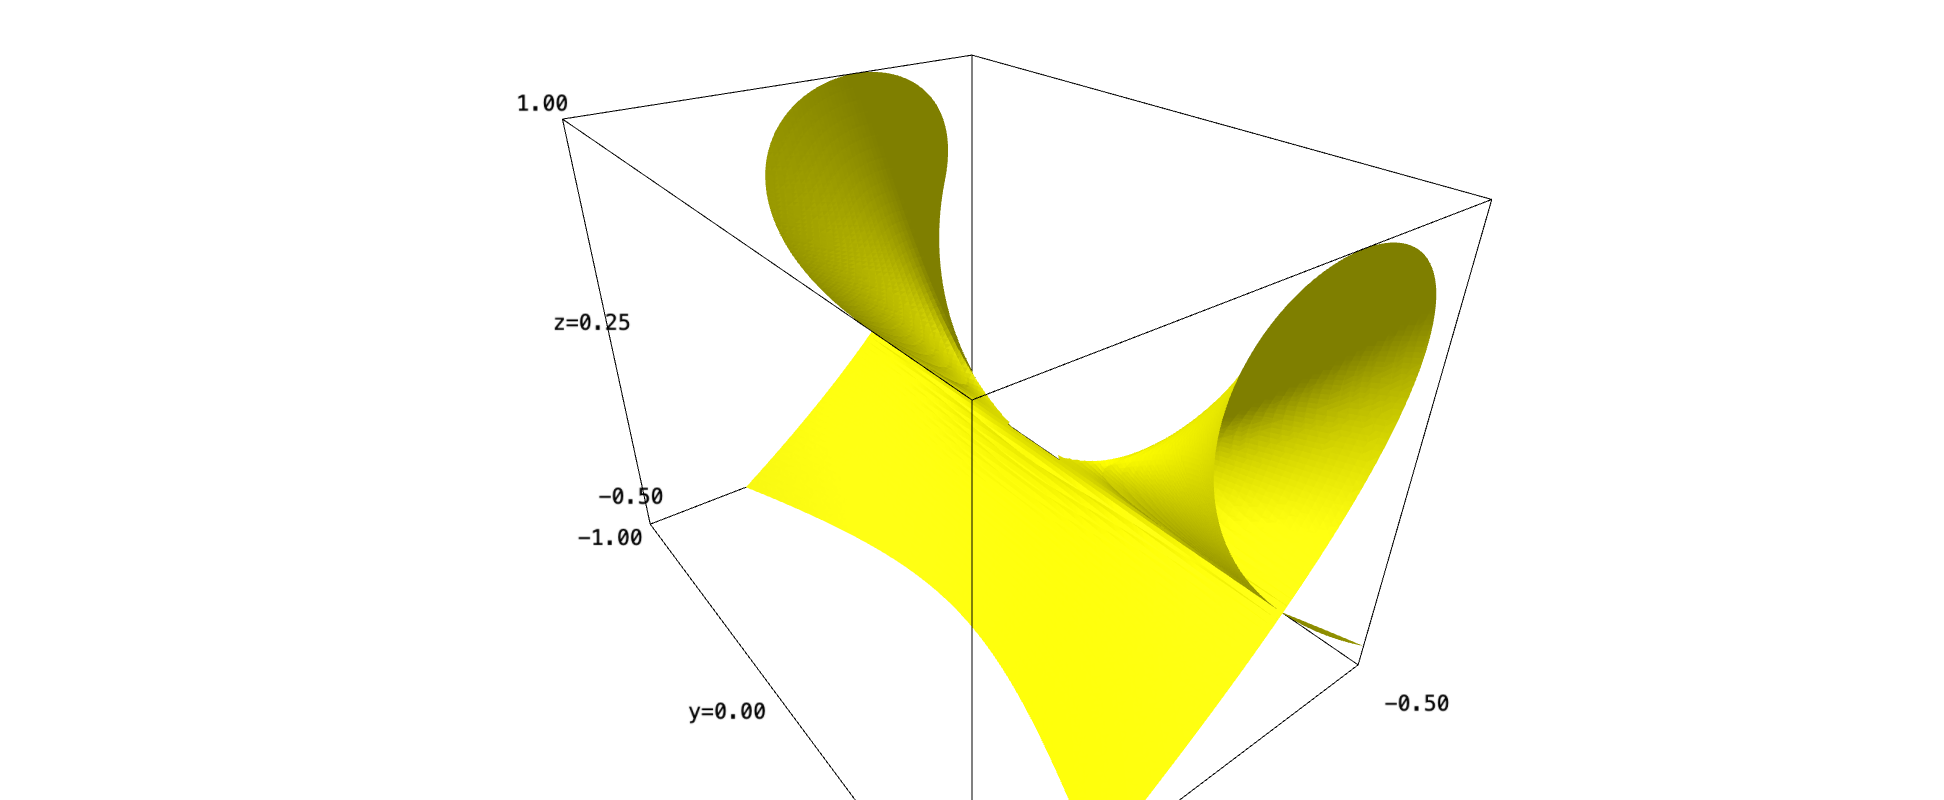
\includegraphics[width=10cm]{example_surface.png}
	\end{center}
	\item $\V(y-x^2, z-x^3)$ ist eine Kurve im drei-dimensionalen affinen Raum, die sogenannte \emph{twisted cubic}. 
	\item $\V(xz,yz)$ ist Vereinigung einer Ebene und einer Geraden. 
	\item Lösungen von lineren Gleichugsystemen in $k^n$ hat man in der linearen Algebra affine Unterräume von $k^n$ genannt. Affine Unterräume sind ebenfalls affine Varietäten. 
	\item Wenn wir für Polynome $f, g   \in \R[x,y,z]$ das Polynom $f(x,y,z)$ unter der Nebenbedingung $g(x,y,z)=0$ optimieren wollen, können wir die sogenannten \emph{Lagrange-Multiplizierer} benutzen, indem wir die  \emph{KKT}-Bedingungen aufstellen (vgl.  Optimierung 1 oder IT-3 für Informatik-Studierende). Wir betrachten also das System 
	\begin{align*}
		\partial_x f - \lambda \, \partial_y g & = 0, 
		\\ \partial_y f - \lambda \,\partial_y g & = 0 , 
		\\ \partial_z f - \lambda \, \partial_z g &= 0,
		\\ g & = 0. 
	\end{align*} 
Dieses System ist durch Polynome aus $\R[x,y,z,\lambda]$ gegeben. Es geht hier also um die Varietät 
$\V( \partial_x f - \lambda \, \partial_y g , \partial_y f - \lambda \, \partial_y g  , \partial_z f - \lambda \,  \partial_z g, g )$. Während man in der nichtlinearen Optimierung die KKT-Bedingungen zur Bestimmung eines lokalen Optimums mit der Verwendung von (lokalen) numerischen Methoden benutzt, kann man natürlich auch fragen, ob man alle lokalen Optima bestimmen kann, um anschließend das globale Optimum bestimmen zu können. Für die Bestimmung \underline{aller }lokalen Optima (ein  schweres Problem) kann man algorithmische Methoden aus Algebra benutzen. 
	\item $\V_\R(x^2 + y^2 + 1)$ ist die leere Menge, $\V_\C(x^2 + y^2 + 1)$ aber nicht. Durch dieses Beispiel wird ersichtlich, dass die Körper wie $\R$ in Algebra zusätzliche Probleme verursachen können, weil sie nicht algebraisch abgeschlossen sind. 
	\item $\V_k(xy,xy-1)$ ist die leere Menge unabhängig von der Wahl des zugrundeliegenden Körpers $k$.
	\item \label{rob:arm}  Betrachten wir die Menge der Zustände eines Roboterarms aus zwei Stangen der Längen $2$ und $1$. Stange der Länge $2$ ist an einem Ende fixiert, die beiden Stangen sind mit einem Gelenk verbunden. Eine algebraische/mathematische Beschreibung eines Modells entsteht oft durch die Einführung von Koordinaten. In diesem Fall:  seien $(0,0), (x,y)$ die beiden Enden der Stange der Länge $2$ und $(x,y)$ und $(z,w)$ die beiden Enden der Stange der Länge $1$. Im gemeinsamen Ende $(x,y)$ hat man ein Gelenk. Nach dem Satz des Pythagoras ist die Menge der Zustände des Roboterarms durch die Gleichungen 
	\begin{align*}
			x^2 + y^2 & = 4,
			\\ (x-z)^2 + (y-w)^2 & = 1.
	\end{align*}
beschrieben. Die Menge der Zustände ist also die Varietät 
\[
	\V_\R(x^2 + y^2 - 4, (x-z)^2 - (y-w)^2 - 1)
\]
im affinen Raum $\R^4$, die man mit zwei Polynomen aus $\R[x,y,z,w]$ beschrieben hat. Diese Varietät ist zwei-dimensional, was intuitiv klar ist. Die Dimension im Sinne der Algebraischen Geometrie müssen wir aber noch formal einführen. Dieses Beispiel deutet  auf eine grundsätzliche Verbindung zur angewandten Mathematik hin: Varietäten können oft als Modelle für Anwendungen benutzt werden. 
\end{enumerate} 
\end{beispiele} 

Die Menge der affinen Varietäten ist abgeschlossen bzgl. endlicher Vereinigungen und Schnitte: 

\begin{lemma}
	Seien $V, W \subseteq k^n$ affine Varietäten. Dann sind auch $V \cup W$ und $V \cap W$ affine Varietäten. 
\end{lemma} 
\begin{proof}
	Wir zeigen, dass für $V = \V(f_1,\ldots,f_s)$ und $W = \V(g_1,\ldots,g_t)$ Folgendes gilt: 
	\begin{align}
			V \cap W & = \V(f_1,\ldots,f_s,g_1,\ldots,g_t), \label{eq:V:cap:W}
	\\		V \cup W & = \V( f_i g_j \, : \, i=1,...s,  \ j=1,\ldots,t). \label{eq:V:cup:W}
	\end{align} 
 Gleichung \eqref{eq:V:cap:W} ist klar. Wir zeigen \eqref{eq:V:cup:W}. 
Sei $a =(a_1,\ldots,a_n) \in k^n$. Ist $a \in V \cup W$ so gilt $f_i(a) =0$ für alle $i =1,\ldots,s$ oder $g_j(a) = 0$ für alle $j=1,\ldots,t$. In den beiden Fällen gilt dann auch $f_i(a) g_j(a)$ für alle $i=1,\ldots,s, \ j=1,\ldots,t$, weil mindestens einer der beiden Faktoren im Produkt $f_i(a) g_j(a)$ gleich $0$ ist. Ist $a \not\in V \cup W$, dann findet man ein $i' =1,\ldots, s$ mit $f_{i'}(a) \ne 0$ sowie ein $j' =1,\ldots,t$ mit $g_{j'}(a)  \ne 0$. Aus $f_{i'} (a) f_{j'}(a) \ne 0$ folgt dann $a \not \in \V ( f_i g_j \, : \, i=1,...s,  \ j=1,\ldots,t).$
\end{proof} 

Nach diesem Beweis kann nun die  Geometrie der Varietät $\V(zx,zy)$, die wir als eines der Beispiele gegeben haben, durch die Umformung $\V(zx,zy) = \V(z) \cup \V(y,z)$ erklärt werden. 

Sei eine affine Varietät $\V(f_1,\ldots,f_s)$ mit  $f_1,\ldots,f_s \in k[x_1,\ldots,x_n]$ gegeben. Unter der Voraussetzung, dass man mit dem zugrundeliegenden Körper konstruktiv (algorithmisch) arbeiten kann, 
sind aus der algorithmischen Perspektive die folgenden Rechen- und Entscheidungsprobleme naheliegend und interessant:

\begin{itemize}
	\item[] \emph{Konsistenz:} Ist $\V(f_1,\ldots,f_s) \ne \emptyset$? Mit anderen Worten geht es hier um die Existenz einer Lösung für ein polynomiales Gleichungssystem. 
	\item[]  \emph{Endlichkeit:} Ist $\V(f_1,\ldots,f_s)$ endlich? Hier geht es um die Endlichkeit der Lösungsmenge eine polynomialen Gleichungssystems. 
	\item[] \emph{Dimension:} Was ist die Dimension von $\V(f_1,\ldots,f_s)$? Wie bereits erwähnt: Hierfür müssen wir zuerst noch den Begriff der Dimension (im Algebraischen Kontext) einführen. 
\end{itemize} 

Für lineare Gleichungssysteme kennen wir algorithmische Lösungen zu allen drei Problemen. Alle diese Probleme können mit Hilfe des Gauß-Verfahrens gelöst werden. (Bzgl. der unendlichen Körper ist die Frage nach der Endlichkeit der Lösungsmenge eines linearen Gleichungssysteme äquivalent zur Frage nach der Eindeutigkeit der Lösung). Wir werden im Laufe dieses Kurses alle drei Fragen beantworten können. 

\begin{aufgaben}{\ }
\begin{enumerate}
	\item Zeigen Sie, dass kein endlicher Körper algebraisch abgeschlossen ist. \textbf{Hinweis:} Klappt es nicht sofort, diese Aussage ganz allgemein zu zeigen, versuchen Sie zuerst konkretere endliche Körper wie $\F_2$, $\F_3$ oder $\F_p$ für eine Primzahl $p$ zu behandeln. 
	\item Zeigen Sie, dass weder der Körper $\Q$ noch der Körper $\R$ algebraisch abgeschlossen sind. 
	\item Wenn Sie noch keinen Beweis des Fundamentalsatzes von Algebra kennen, finden Sie einen einfachen Beweis und versuchen Sie ihn zu verstehen. 
	\item Zeigen Sie, dass jede endliche Teilmenge von $k^n$ eine affine Varietät ist. 
	\item Entscheiden Sie für die Mengen $ \R \setminus \{0\} $, $\R^2 \setminus \{(0,0)\}$, $\R \times \R_{>0}$, $\R \times \R_{\ge 0}$, ob sie affine Varietäten bzgl. des Körpers $\R$ sind. Begründen Sie Ihre Aussagen. 
	\item Zeigen Sie, dass der Durchschnitt und die Vereinigung endlich vieler affinen Varietäten ebenfalls affine Varietäten sind. Wir werden später sehen, dass der Durchschnitt beliebiger Anzahl affiner Varietäten eine affine Varietät ist. Wie sieht es aber mit der Vereinigung beliebiger Anzahl affiner Varietäten aus? 
	\item Seien $V \subseteq k^n$ und $W \subseteq k^m$ affine Varietäten. Man zeige, dass $V \times W \subseteq k^{n +m}$ ebenfalls eine affine Varietät ist. 
\end{enumerate}
\end{aufgaben} 

\subsection{Parametrisierung und Implitisierung affiner Varietäten}

In diesem Abschnitt wollen wir auf am Beispiel der Parametrisierung und Implitisierung ein Beispiel zu möglichen Anwendungen der Methoden von Algebra geben. Um parallelen mit der linearen Algebra zu ziehen, beginnen wir mit Parametrisierung und Implitisierung im Fall von affinen Unterverktorräumen. 

\begin{beispiel} 
Mit Parametrisierung affiner Unterräume hatte man indirekt in der linearen Algebra zu tun. Wenn wir zum Beispiel eine affinen Unterraum $U$ von $k^3$ als die Lösungsmenge von 
\begin{align*}
		x + y + z & = 1,
\\		x + 2y - z & = 3
\end{align*}
festgelegt haben, so können wir eine parametrische Darstellung davon mit Hilfe des Gauß-Verfahrens  herleiten. Dafür überführen wir das System in eine reduzierte Stufenform: 
\begin{align*}
		\textbf{x}+ 3 z & = -1,
\\		\textbf{y} - 2z & = 2.
\end{align*}
Daraus ergibt sich die parametrische Darstellung, bei der die Variable $z$ als ein Parameter benutzt wird: 
\[
	U = \setcond{ (-1-3t,2 + 2t, t) }{t \in k}
\] 
\end{beispiel} 

\begin{remark} 
Umgekehrt können wir aus einer parametrischen Darstellung eines affinen Unterraums $U$ von $k^n$ eine Beschreibung als lineares Gleichungssystem herleiten. Dafür kann man ebenfalls das Gauß-Verfahren benutzten. Überlegen Sie sich, wie das genau geht. \textbf{Hinweis:} Eine Parametrisierung kann ist durch ein System von Gleichungen $ x = A t + b$ in zwei Gruppen von Variablen $x$ und $t$ darstellbar, wobei die Gruppe $t$ zur Parametrisierung einer Mengen im Raum der $x$-Variablen benutzt wird. Welchen Nutzen hat die Anwendung des Gauß-Verfahrens bzgl. der $t$-Variablen? 
\end{remark} 

\begin{beispiel}[Rationale Parametrisierung des Kreises]
In der Algebraischen Geometrie benutzt man oft die sogenannte rationale Parametrisierung von Varietäten. Die genaue Definition werden wir in Kürze geben, es bietet sich aber an, vorbereitend zur Definition eine rationale Parametrisierung des Kreises  $x^2 + y^2  =1$ herzuleiten. Dieser hat die rationale parametrische Beschreibung 
\begin{align*}
		x  & = \frac{1-t^2}{1+t^2}, 
&		y & = \frac{2t}{1 + t^2}.
\end{align*}
Die Idee hinter dieser Beschreibung ist wie folgt. Die Schar aller Geraden, die den Punkt $(-1,0)$ des Kreises $\V(x^2 + y^2 - 1)$ enthalten lässt sich fast vollständig parametrisieren, da wir alle Geraden dieser als die Varietäten, bis auf die vertikale Gerade $\V(x+1)$ als $\V(y - t (x+1))$ mit Hilfe eines Parameters $t$ parametrisieren können. Durch das Einsetzen von $y = t (x+1)$ in die Gleichung $x^2 + y^2 -1 =0$ des Kreises, erhält man die Gleichung $x^2 + t^2 (x+1)^2  - 1 =0$. Die linke Seite dabei ist für jedes festes $t$ ein quadratisches Polynom in $x$. Das Polynom hat $x=-1$ als eine der Nullstellen. Diese Nullstelle entspricht dem Schnittpunkt $(-1,0)$ unserer parametrisierten Gerade und des Kreises. Die anderen Nullstelle, die wir ebenfalls bestimmen können, entspricht dem anderen Schnittpunkt. Diesen anderen Schnittpunkt kann man durch das Faktorisieren von $x^2 + t^2 (x+1)^2 -1$ ermitteln. Wir haben 
\begin{align*}
		x^2 + t^2 (x+1)^2 - 1 & = (x-1) (x+1) + t^2 (x+1) (x+1) 
		\\ & = (x+1) ( x-1 + t^2  (x+1)). 
\end{align*} 
Der andere Schnittpunkt ergibt sich also durch das Auflösen der Gleichung 
\[
	x-1 + t^2 (x+1) =0 
\]
nach $x$. Man erhält $x = (1-t^2) / (1+t^2)$. Das Einsetzen von $x$ in die Gleichung $y = t (x+1)$ der geraden legt $y = 2 t / (1+t^2)$ in Abhängigkeit vom Parameter $t$ fest. 

In welchem Zusammenhang befinden sich der Kreis $C=\V_\R(x^2 + y^2 -1)$ und die Menge $C'= \setcond{\left( \frac{1-t^2}{1+t^2} ,  \frac{2t}{ 1 + t^2} \right) } { t\in\R}$? 

Für die so ermittelte Parametrisierung kann man nun formal begründen, dass diese tatsächlich eine Parametrisierung im Sinne der 

Wegen der Gleichung $(1-t^2)^2 + (2t)^2 = (1+t^2)^2$ ist $C' \subseteq C$. 
 Zum Punkt $(-1,0) \in C$ aus dem Kreis findet man aber kein passendes $t$, woraus man die verstärkte Inklusion $C' \subseteq C \setminus \{(-1,0)\}$ folgert. Auch die umgekehrte Inklusion ist erfüllt, da wir für jeden Punkt aus $p \in C \setminus \{(-1,0)\}$ als das passende $t$ die Neigung der Geraden durch die Punkte $(-1,0)$ und $p$ festlegen können. Wir erhalten die Gleichheit  $\V_\R(x^2 + y^2 - 1) \setminus \{(-1,0)\} = \setcond{ \left( \frac{1-t^2}{1+t^2} ,  \frac{2t}{ 1 + t^2} \right) }{t \in \R}$ und sehen an diesem Beispiel, dass man wohl bei der rationalen Parametrisierung nicht die exakte Beschreibung sondern etwas schwächere Eigenschaft meinen soll. 
\end{beispiel} 

\begin{definition}[Rationale Funktionen]
Formale Quotienten von Polynomen nennt man in der Algebra und Algebraischer Geometrie \emph{rationale Funktionen}. Das Wort Funktion in diesem Begriff ist eigentlich eine Fehlbezeichnung, denn rationale Funktionen sind im Allgemeinen keine Funktionen, sondern genauso wie Polynome formale Ausdrücke. 

Genauer ist die Menge aller rationalen Funktionen in den Unbestimmten $x_1,\ldots,x_n$ und mit Koeffizienten im Körper $k$ als die Menge der formalen Quotienten $f/g$ mit $f \in k[x_1,\ldots,x_n]$ und $g \in k[x_1,\ldots,x_n] \setminus \{0\}$ definiert. 

Man bezeichnet diese Menge als $k(x_1,\ldots,x_n)$. Die Gleichheit von zwei Quotienten $f/g$ und $u/v$ mit $f,u \in k[x_1,\ldots,x_n]$ und $g,v \in k[x_1,\ldots,x_n] \setminus \{0\}$ ist durch die polynomiale Gleichung $f v = g u$ definiert.\footnote{Genauso wie $k(x_1,\ldots,x_n)$ aus $k[x_1,\ldots,x_n]$ entsteht, entsteht die Menge $\Q$ der rationalen Zahlen aus der Menge $\Z$ der ganzen Zahlen.} Den Polynomring $k[x_1,\ldots,x_n]$ interpretiert man als Teilmenge von  $k(x_1,\ldots,x_n)$, da man jedes $f \in k[x_1,\ldots,x_n]$ als den Quotienten $f/1$ schreiben kann. Des Weiteren werden in $k(x_1,\ldots,x_n)$ die binären Verknüpfungen Addition und Multiplikation auf die folgende naheliegende Weise eingeführt: 
\begin{align*}
		\frac{f}{g}  + \frac{u}{v} & : = \frac{f v + u g}{gv},
		\\ \frac{f}{g} \cdot \frac{u}{v} & := \frac{f u}{g v}. 
\end{align*} 
\end{definition} 
Man beachte, dass die Addition und Multiplikation von rationalen Funktionen wohldefiniert ist, weil dass Produkt $g v$ von zwei Nichtnullpolynomen ein Nichtnullpolynom ist (warum?). 

\begin{remark} 
Wir bemerken auch, dass $k(x_1,\ldots,x_n)$ bzgl. der Addition und Multiplikation einen Körper bildet. Dass das ein kommutativer Ring mit $1$ ist, ist nicht schwer zu sehen. Wir sehen aber auch, dass zusätzlich ein Nichtnullelement aus $k(x_1,\ldots,x_n)$, also eine rationale Funktion $f/g$ mit $f,g \in k[x_1,\ldots,x_n] \setminus \{0\}$, stets invertierbar ist, denn $f/g \cdot g/f = 1$. 
\end{remark} 

\begin{definition} 
Sei $V \subseteq k^n$ sind $p_1,\ldots,p_n \in k[t_1,\ldots,t_m]$ und $q \in k[x_1,\ldots,x_n] \setminus \{0\}$ derart, dass $V$ die inklusionskleinste affine Varietät, welche die Menge 
\[
	\setcond{ (p_1(b)/ q(b),\ldots,p_n(b)/q(b)) }{b \in k^m, \ q(b) \ne 0}
\]
als Teilmenge enthält, so nennen wir die Beschreibung 
\begin{align*}
	x_1 & = p_1(t_1,\ldots,t_m) / q(t_1,\ldots,t_m), 
	\\ & \vdots 
	\\ x_n & = p_n(t_1,\ldots,t_m) / q(t_1,\ldots,t_m)
\end{align*} 
eine rationale parametrische Darstellung von $V$. Im Fall $q=1$, nennen wir diese Beschreibung eine polynomiale parametrische Darstellung. 
\end{definition} 

\begin{definition} 
Man nennt  die Beschreibung $V = \V(f_1,\ldots,f_s)$ als die Lösungsmenge vom Polynomialen System $f_1 = \cdots  = f_s =0$ eine \emph{implizite Darstellung} von $V$. 
\end{definition} 

Jede affine Varietät hat laut der Definition eine implizite Darstellung. Es stellt sich heraus, dass nicht jede affine Varietät rational parametrisierbar ist. Wir werden aber sehen, dass jede rationale parametrische Darstellung ``implitisiert werden kann''. Das heißt: für jede Angabe von $p_1,\ldots,p_n \in k[t_1,\ldots,t_m]$ und $q \in k[t_1,\ldots,t_m]  \setminus \{0\}$ gibt es eine affine Varietät, die als $x_1 = p_1/q,\ldots, x_n = p_n/q$ parametrisch beschrieben ist. Die Implizite Beschreibung als $f_1 = \cdots = f_s =0$ kann algorithmisch ermittelt werden. 

Zunächst betrachten wir aber einige Beispiele: 

\begin{beispiele} {\ } 
\begin{enumerate} 
	\item Die Varietät zur Gleichung $x^2 - y^2 z^2 + z^3 =0$ kann parametrisch als 
\begin{align*}
		x & = t (u^2 - t^2),  &  y & =u,  &  z & = u^2 - t^2
\end{align*} 
beschrieben werden. 
Wenn unsere Varietät nur parametrisch gegeben wäre, müssten wir zum Testen, ob ein konkreter Punkt wie $(1,2,-1)$ zur Varietät gehört, ein polynomiales Gleichungssystem lösen. Anhand  der impliziten Darstellung kann so ein Test direkt durchgeführt werden, indem man $x=1, y=2, z=-1$ einsetzt. Parametrisierung sind wiederum für manche andere Dinge nützlich. Wenn man beispielsweise den Roboterarm aus Beispiel~\ref{bsp:var}\eqref{rob:arm} betrachten, so könnte man den Arm mit zwei Parametern beschreiben wollen, um dann ihn durch die Angabe dieser Parameter steuern zu können. Wenn man über einer Varietät $\V_\R(f_1,\ldots,f_s)$ ein Polynom $g$ optimieren möchte, so kann man durch eine polynomiale Parametrisierung $x_i = p_i(t_1,\ldots,t_m)$ (vorausgesetzt, dass  sie vorhanden ist), auf die nicht-restringierte Optimierung des Polynoms $g(p_1(t_1,\ldots,t_m),\ldots,p_n(t_1,\ldots,t_m)) \in \R[t_1,\ldots,t_m]$ über $\R^m$ zurückführen, was in eine Vereinfachung der Originalaufgabe resultieren kann. 

	\item Die Kurve $C=\V(y -x^2, z-x^3, w - x^4)$ im Raum $k^4$ kann offensichtlich als $\setcond{ (t,t^2, t^3,t^4) }{t \in k}$ parametrisch beschrieben werden. Diese Beobachtung kann im Fall $k=\R$ benutzt werden um die Optimierung eines Polynomas $f \in k[t]$ vom Grad $4$ als eine Optimierung einer linearen Funktionen über die Kurve $C$ zu interpretieren (solche geometrische Interpretationen können oft sehr hilfreich sein). 
	
	\item Implizite Beschreibung der Fläche die zusammen mit jedem Punkt von $\V_\R(y - x^2, z - x^3)$ die Tangente an diesem Punkt enthält können wir aus der offensichtlichen parametrischen Beschreibung 
	\begin{align*}
			x & = t + 2 u 
		\\	y & = t^2 + 2 t u
		\\	z & = t^3 + 3  t^2 u 
	\end{align*} 
	ermitteln. Wir sehen etwas später wie. 
	\item Bei B\'ezier-Splines handelt es sich um die parametrische Beschreibung der Kurven $ \setcond{ (1-t)3 p_0 + 3 t (1-t)^2 p_1 + 3 t^2 (1-t) + t^3  p_3 }{t \in \R}$ durch die Angaben von $p_0,\ldots,p_3 \in \R^2$, wobei hier durch Polynome aus $\R[t]$ vom Grad höchstens $3$ parametrisiert wird. 
\end{enumerate} 
\end{beispiele} 

Die folgende Proposition beschreibt die Situation im linearen Fall. 

\begin{proposition}[Parametrisierung und Implitisierung im linearen Fall]
	\label{prop:param:affin} 
	Für affine Unterraume von $k^n$ gilt Folgendes: 
\begin{itemize}
	\item[] \emph{Parametrisierung:} Die Lösungsmenge $X=\setcond{x \in k^n}{A x =b}$ eines linearen Gleichungssystems $A x =b$, mit $A \in k^{m \times n}$ und $b \in k^m$, falls sie nicht leer ist, kann in einer parametrischen Form als 
	\[ 
		X=\setcond{U t + v}{t \in k^s},
	\]
	mit $U \in k^{n \times s}$,  $v \in k^n$ und $s \in \{1,\ldots,n\}$, beschrieben werden. Es gibt einen Algorithmus, der $U$ und $v$ für gegebene $A$ und $b$ berechnet. 
	\item[] \emph{Implitisierung:} Die Menge $X=\setcond{ U t + v}{t \in k^s}$, mit $ U \in k^{n \times s}$ und $v \in k^n$, kann in einer impliziten Form als  
	\[ 
		X=\setcond{x \in \R^n}{A x = b},
	\] mit $A \in k^{m \times n}$ und $b \in k^m$ und $m \in \{1,\ldots,n\}$,  beschrieben werden. Es gibt einen Algorithmus, für $A$ und $b$ für gegebene $U$ und $v$ berechnet. 
\end{itemize} 	
\end{proposition} 
\begin{proof}
	Aufgabe.  
\end{proof} 


\begin{aufgaben} {\ }
	\begin{enumerate} 
		\item Warum ist das Produkt von zwei Nichtnullpolynome ein Nichtnullpolynom? 
		\item Beweisen Sie Proposition~\ref{prop:param:affin}
		\item Finden Sie eine implizite Beschreibung der affinen Varietät  $V \subseteq \R^2$ mit der Parametrisierung $x = \frac{t}{1+t^2}, y = 1- \frac{1}{t^2}$. Versuchen Sie sauber zu begründen, dass  dass tatsächlich die Parametrisierung der von Ihnen gefundenen Varietät $V$ ist. 
		\item Finden Sie eine rationale Parametrisierung der Sphäre $x^2 + y^2 + z^2 =1$ in $\R^3$. Versuchen Sie dabei die Idee der Parametrisierung eines Kreises zu benutzen. 
		\item Finden Sie eine rationale Parametrisierung der Kurve $y^2 = x^2 - x^3$. Die Idee hinter der Parametrisierung des Kreises kann auch in diesem Fall benutzt werden. 
	\end{enumerate} 
\end{aufgaben} 


\subsection{Ideale} 

Ideale kann man ganz allgemein für kommutative Ringe einführen. Wir beschränken uns hier auf Ideale des Rings $k[x_1,\ldots,x_n]$, obwohl man den Begriff eines Ideals genau so, wie wir es nachfolgend einführen bzgl. eines beliebigen kommutativen Rings einführen könnte: 

\begin{definition} Eine Teilmenge $I$ von $k[x_1,\ldots,x_n]$ nennt man ein Ideal, wenn Folgendes erfüllt ist: 
\begin{enumerate}[(a)]
	\item $0 \in I$
	\item Für alle $f,g \in I$ gilt $f+g \in I$. 
	\item Für alle  $h \in k[x_1,\ldots,x_n]$ und $f \in I$  gilt $hf  \in I$. 
\end{enumerate} 
\end{definition} 

Vielleicht erinnert Sie die vorige Definition ein bisschen an die Definition eines Untervektorraums. Die erste und die zweite Bedingungen sehen bei der Definition von Untervektorräumen genauso aus. In der dritter Bedingung wäre aber bei Vektorräumen $h$ ein Element des Körpers $k$. In dieser Definition ist das $h$ ein Polynom aus $k[x_1,\ldots,x_n]$. 

Sehr oft werden Ideale durch die Angabe der Erzeuger generiert: 

\begin{definition}
	Für $f_1,\ldots,f_s \in k[x_1,\ldots,x_n]$ nennen wir 
	\[
		\ideal{ f_1,\ldots,f_s}  :=  \setcond{ h_1 f_1 + \cdots + h_s f_s }{h_1,\ldots,h_s \in k[x_1,\ldots,x_n]}
	\]
	das durch $f_1,\ldots,f_s$ erzeugte Ideal. 
\end{definition} 

Bestimmt erinnert Sie die vorige Definition an die Definition der linearen Hülle. In diesem Fall hat man aber als ``Koeffizienten'' Polynome $h_1,\ldots,h_s$ und nicht die Elemente aus $k$. Wir müssen den Namen `erzeugte Ideal' rechtfertigen. Es ist tatsächlich ein Ideal: 

\begin{lemma}
	Seien $f_1,\ldots,f_s \in I$. Dann ist $\ideal{f_1,\ldots,f_s}$ ein Ideal. 
\end{lemma} 
\begin{proof} 
	Sei $I := \ideal{f_1,\ldots,f_s}$. Wir verifizieren für $I$ die definierenden Eigenschaften eines Ideals. 
	Es gilt $0 = 0 \cdot f_1 + \cdots + 0 \cdot f_s \in I$
	Für zwei beliebige Elemente $u = h_1 f_1 +  \cdots + h_s f_s$ und $v = g_1 f_1 + \cdots + g_s f_s$ aus $I$ mit $h_1,\ldots,h_s, g_1,\ldots, g_s \in k[x_1,\ldots,x_n]$ gilt für ihre Summe 
	\[
		a + b = (h_1 + g_1) f_1 +  \cdots + (h_s + g_s) f_s \in I. 
	\]
	Des Weiteren gilt für  $u \in I$ wie oben und ein beliebiges $w \in k[x_1,\ldots,x_n]$ 
	\[
		w u = (w h_1) f_1 + \cdots + (w h_s) f_s \in I. 
	\]
\end{proof}

Aus dem Gleichungssystem $f_1 = \cdots = f_s =0$ folgt natürlich die Gleichung $g=0$ mit $g \in \ideal{f_1,\ldots,f_s}$. Diese einfache aber grundlegende  Beobachtung verlinkt Ideale mit den Varietäten und dem Lösen von polynomialen Gleichungssystemen. 

\begin{beispiel}
Hier eine Illustration, wie man Ideale potenziell  zum Implitisieren einsetzen könnte: 
Wir betrachten die parametrisierte Darstellung $x=t, y=t^2, z=t^3$ einer Kurve. Dazu führen wir das Ideal $\ideal{x-t,y-t^2, z-t^3} \subseteq k[x,y,z,t]$ ein. Aus dem Ideal kann man die Gleichungen $y = x^2$ und $z = x^3$ ablesen, denn
\begin{align*}
	(x+t) \cdot (x-t) + (-1) \cdot (y-t^2) & = x^2 - y,
	\\ (x^2 + x t + t^2) \cdot (x-t) + (-1) \cdot (z - t^3) & = x^3 - z. 
\end{align*}
\end{beispiel}

\begin{definition}
Ein Ideal $I \subseteq k[x_1,\ldots,x_n]$ nennt man \emph{endlich erzeugt}, wenn $I = \ideal{f_1,\ldots,f_s}$ für gewisse endlich viele $f_1,\ldots,f_s \in k[x_1,\ldots,x_n]$ gilt. In diesem Fall sagt man, dass $f_1,\ldots,f_s$ eine \emph{Basis} von $I$ ist. 
\end{definition} 

Man beachte, dass Basen von Idealen nicht analog zu den Basen der Vektorräume definiert werden, sondern analog zu den Erzeugendensystemen. 

Im nächsten Kapitel wird eine sehr bemerkenswerte Tatsache bewiesen: jedes Ideal von $k[x_1,\ldots,x_n]$ ist endlich erzeugt. Dieses Resultat nennt man das Hilbert-Basis-Theorem. 

Nun geben wir einen weiteren Kommentar über den Zusammenhang von Idealen und Varietäten: die Lösungsmenge von $f_1 = \cdots = f_s =0$ ist durch das Ideal $\ideal{f_1,\ldots,f_s}$ eindeutig bestimmt. Das bedeutet, dass man die Varietäten statt als Funktionen $\V(f_1,\ldots,f_s)$ eines Vektorsystems $\{f_1,\ldots,f_s\}$ als Funktionen $\V(I)$ eines Ideals auffassen kann. 

\begin{proposition}
	Für alle  $f_1,\ldots,f_s,g_1,\ldots,g_t \in k[x_1,\ldots,x_n]$ mit $\ideal{f_1,\ldots,f_s} = \ideal{g_1,\ldots,g_t}$ gilt $\V(f_1,\ldots,f_s) = \V(g_1,\ldots,g_t)$. 
\end{proposition} 
\begin{proof}
	Aufgabe. 
\end{proof} 

Nach der vorigen Proposition gilt: wenn man die Basis eines Ideals wechselt ohne das Ideal zu ändern, macht man eine äquivalente Umformung eines polynomialen Gleichungssystems. Diese Beobachtung wird für die nachfolgenden algorithmischen Überlegungen wichtig sein. 

Wir haben bisher einem polynomialen Gleichungssystem $f_1= \cdots = f_s=0$ die Lösungsmenge $\V(f_1,\ldots,f_s)$ und das Ideal $\ideal{f_1,\ldots,f_s}$ zugeordnet. Wir haben festgestellt, dass $\V(f_1,\ldots,f_s)$ nur vom Ideal abhängig, das heißt, man hat die Abbildungen 
\[
	(f_1,\ldots,f_s) \mapsto \ideal{f_1,\ldots,f_s} \mapsto \V(f_1,\ldots,f_s). 
\]

In der folgenden Definition wird die Verbindung in die anderen Richtung erstellt. Und zwar wird einer Teilmengen von $k^n$ ein Ideal zugeordnet. 

\begin{definition} 
	Für $X \subseteq k^n$ heißt
	\[
		 \I(X) := \setcond{ f \in k[x_1,\ldots,x_n] }{ f(a) = 0 \ \text{für alle} \ a \in X}
	\]
	das Ideal von $X$. 	
\end{definition} 

Wir zeigen, dass die vorige Menge tatsächlich ein Ideal ist. 

\begin{lemma} 
	Sei $X \subseteq k^n$. Dann ist $\I(X)$ ein Ideal. 
\end{lemma} 
\begin{proof}
	Aufgabe. 
\end{proof} 

Uns interessieren vor allem die Ideale von Varietäten. Wir betrachten einige Beispiele: 

\begin{beispiele}{\ } 
\begin{enumerate}
	\item Für $V = \{(0,0) \}$ ist $\I(V) = \ideal{x,y}$. Da eine der beiden Inklusion trivial ist,  müssen wir lediglich die Inklusion $\subseteq$ verifizieren. Die Bedingung $f(x,y) \in \I(V)$ heißt, $f(0,0)=0$. Wir können $f$ als $A(x,y)x + B(x,y) y + C$ mit $A,B \in k[x,y]$ und $C \in k$ schreiben. Da man $f(0,0) =0$ hat, gilt $C=0$. Daraus folgt $f \in \ideal{x,y}$. 
	\item $\I(k^n) =\{0\}$ für unendliche Körper $k$. Das ist eine Umformulierung von Proposition~\ref{prop:nullpolynom}.  
	\item Ein weniger triviales Beispiel ist $V = \V_\R(y-x^2, z -x^3)$. Wir zeigen, dass in diesem Fall $\I(V) = \ideal{y - x^2, z - x^3}$ gilt. Ein beliebiges $f \in \R[x,y,z]$ kann als $f = h_1 (y-x^2)+ h_2 (z-x^3) + r$ mit $h_1,h_2 \in \R[x,y,z]$ und dem ``Rest'' $r \in \R[x]$, der nur von $x$ abhängig ist, dargestellt werden. Um das zu sehen, reicht es diese Darstellung für alle Monome $f = x^\alpha y^\beta z^\gamma$ zu finden. Wenn wir eine solche Darstellung für die Monome mit $\alpha =0$ finden, finden wir sie auch für alle anderen Monome. Wir können also $\alpha =0$ setzen. Es geht also um den Fall $f = y^\beta z^\gamma$. Es gilt 
	\begin{align*}
			y^\beta z^\gamma = ((y-x^2) + x^2)^\beta ( (z-x^3) + x^3)^\gamma. 
	\end{align*}
	Das Ausmultiplizieren der beiden Klammern mit der Verwendung des binomischen Lehrsatzes ergibt eine Darstellung als Summe mit den Termen, die $(y-x^2)$ oder $(z-x^3)$ als Faktor enthalten oder sonst nur von $x$ abhängig sind. Das zeigt die gewünschte Behauptung. Nun können wir 
	die Gleichung $\I(V)= \ideal{y-x^2, z- x^3}$ zeigen. Nur die Inklusion $\subseteq$ ist nichtrivial. Sei $f \in k[x,y,z]$ gleich $0$ auf $V$. Wir zerlegen $f$ als $f = h_1 (y-x^2) + h_2(z-x^3) + r$. Da $V$ alle Punkte der Form $(t,t^2,t^3)$ erhält, folgt daraus, dass $r(t)=0$ für alle $t \in k$ ist. Da der Körper $\R$ unendlich ist, ist $r(x)$ ein Nullpolynom. Es folgt $f \in \ideal{y-x^2,z-x^3}$. 
\end{enumerate} 
\end{beispiele} 

Als Nächstes vergleichen wir das Ideal $\ideal{f_1,\ldots,f_s}$ mit dem Ideal $\I(\V(f_1,\ldots,f_s))$.  Das erste Ideal ist die Menge der ``Linearkombinationen'' von $f_1,\ldots,f_s$ mit polynomialen ``Koeffizienten''. Das zweite Ideal beschreibt die Menge aller polynomialen Gleichungen $g =0$ die aus dem System $f_1 =\cdots = f_s=0$ folgen.  
Im Fall der Gleichheit $\ideal{f_1,\ldots,f_s} = \I(\V(f_1,\ldots,f_s))$ kann jede Polynomiale Gleichung, die aus $f_1 = \cdots = f_s =0$ folgt vom Ideal $\ideal{f_1,\ldots,f_s}$ abgelesen werden. So einen günstigen Fall hatten wir zum in unserem Beispielsystem $y - x^2 = z-x^3 =0$. Diese günstige Bedingung gilt aber im Allgemeinen nicht: 

\begin{lemma} 
	Für alle $f_1,\ldots,f_s \in k[x_1,\ldots,x_n]$ gilt $\ideal{f_1,\ldots,f_s} \subseteq \I(\V(f_1,\ldots,f_s))$. Des Weiteren existieren $f_1,\ldots,f_s \in k[x_1,\ldots,x_n]$, für welche die vorige Inklusion strikt ist. 
\end{lemma} 
\begin{proof}
	Die Inklusion ist klar. Die Inklusion ist strikt für $s=1$ mit $f_1 = x_1^2$, denn Polynom $x_1$ gehört zum Ideal $\I(\V(x_1^2))$, aber nicht zum Ideal $\ideal{x_1^2}$. 
\end{proof} 

Für allgemeine Körper kann der Zusammenhang von $\ideal{f_1,\dots,f_s}$ und $\I(\V(f_1,\ldots,f_s))$ sehr subtil sein. Für $k = \C$ werden wir aber eine Operation einführen, durch welche man $\I(\V(f_1,\ldots,f_s))$ aus $\ideal{f_1,\ldots,f_s}$ konstruieren kann. Das ist der Gegenstand vom Nullstellensatz aus dem Kapitel~4. 

Zunächst werden wir eine Beobachtung über das Verhalten von $\I(V)$ bzgl. der Inklusion formulieren. 

\begin{proposition} \label{prop:var:vs:ideal}
	Seien $V, W \subseteq k^n$ affine Varietäten. Dann gilt 
	\begin{enumerate}[(i)]
		\item Aus $V \subseteq W$ folgt $\I(V) \supseteq \I(W)$. 
		\item $V=W$ is äquivalent zu $\I(V)=\I(W)$. 
	\end{enumerate} 
\end{proposition} 
\begin{proof}
	(i) folgt direkt aus der Definition vom Ideal einer Menge. Wir zeigen (ii). Ist $V=W$, so gilt trivialerweise $\I(V) = \I(W)$. Umgekehrt sei $\I(V)= \I(W)$. Sei $V =\V(f_1,\ldots,f_s)$ und $W = \V(g_1,\ldots,g_t)$. Die Gleichheit $\I(V) = \I(W)$ heißt, dass jedes Polynom, das auf $V$ gleich $0$ ist auch auf $W$ gleich $0$ und umgekehrt. Somit sind die Polynome $f_1,\ldots,f_s$ auf $W$ gleich $0$ und die Polynome $g_1,\ldots,g_t$ auf $V$ gleich $0$. Somit hat die Lösungsmenge $V$ von $f_1 = \cdots =f _s=0$ die Menge $W$ als Teilmenge und umgekehrt. Das zeigt $V=W$. 
\end{proof} 

\begin{aufgaben}{\ } 
\begin{enumerate}
	\item Man betrachte das System 
	\begin{align*} 
			x^2 + y^2 - 1 & = 0,  & xy - 1 & = 0.
	\end{align*} 
	Bestimmen Sie eine Gleichung $f(x) = 0$ mit $f \in k[x] \setminus \{0\}$, die aus diesem System folgt. Liegt Ihr $f$ in $\ideal{x^2 + y^2 -1, xy -1}$? 
	\item Sei $I$ Ideal und seien $f_1,\ldots,f_s$ Polynome. Zeigen Sie die Äquivalenz von $f_1,\ldots,f_s \in I$ und $\ideal{f_1,\ldots,f_s} \subseteq I$. 
	\item Zeigen Sie die folgenden Gleichungen für Ideale des Rings $k[x,y]$: 
	\begin{align*}
			\ideal{x+y,x-y} & = \ideal{x,y} = \ideal{x^2 + xy, y + xy, x^2, y^2},
			 \\ \ideal{2 x^2 + 3 y^2 - 11, x^2 - y^2 -3} & = \ideal{x^2 -4, y^2 - 1}. 
	\end{align*}
	\item Man zeige $\V(x + xy, y + xy, x^2, y^2) = \V(x,y)$. 
	\item Man nennt eine Basis eines Ideals minimal, wenn sie inklusionsminimal ist: das heißt, jede echte Teilmenge der Basis erzeugt ein anderes (kleineres) Ideal. Zeigen Sie $I:=\ideal{x} = \ideal{x + x^2, x^2}$. Zeigen Sie, dass die beiden Basen $x$ und $x+x^2,x^2$ vom Ideal $I$ minimal sind. 
	\item Ein Ideal $I$ nennt man Radikalideal, wenn für jedes $f \in k[x_1,\ldots,x_n]$ und jedes $m \in \Z_{>0}$ aus $f^m \in I$ die Bedingung $f \in I$ folgt. Man zeige, dass das Ideal $\I(X)$ einer Menge $X \subseteq k^n$ stets ein Radikalideal ist. 
	\item Zeigen Sie, dass $V:=\setcond{(t,t^3,t^4)}{t \in k}$ eine affine Varietät ist, und bestimmen Sie eine Basis von $\I(V)$. 
	\item Zeigen Siee, dass $V:= \setcond{(t^2,t^3,t^4)}{t \in k}$ eine affine Varietät ist, und bestimmen Sie eine Basis von $\I(V)$. 
	\item Zeigen Sie, dass für $\F_2[x,y]$ die Gleichung $\I(\F_2^2) = \ideal{x^2 -x,y^2 -y}$ erfüllt ist. Das heißt, jedes Polynom $f \in \F_2[x,y]$, das auf dem gesamten $\F_2^2$ gleich $0$ ist, gehört zum Ideal $\ideal{x^2-x,y^2 -y}$. 
	\item Man bestimme das Ideal $\I(\Z^n)$ bzgl. $k= \C$. 
\end{enumerate}
\end{aufgaben}

\subsection{Polynome in einer Variablen} 

In diesem Abschnitt erledigen wir den univariaten Fall der meisten Fragen, die wir oben formuliert haben. In algorithmischen Aussagen, gehen wir davon aus, dass wir die in unseren Algorithmen auf Addition, Subtraktion, Multiplikation und Division im Körper $k$ zugreifen können. 

\begin{definition}
	Sei $f = a_0 x^m + a_1 x^{m-1} + \cdots + a_m \in k[x] \setminus \{0\}$ mit $a_0 \in k\setminus \{0\}$, $a_1,\ldots,a_m \in k$. Wir nennen $a_0 x^m$ den Leitterm von $f$ und benutzen dafür die Bezeichnung $\LT(f)$. 
\end{definition} 

Polynome in einer Variablen kann man mit Rest dividieren: 

\begin{proposition}\label{prop:div:rest}
	Für jedes $f \in k[x]$ und $g \in k[x] \setminus \{0\}$ existiert eine eindeutige Darstellung 
	\[
		f = q \cdot g + r
	\]
	mit $q,r \in k[x]$ und $\deg(r) < \deg(g)$ (Den Grad vom Nullpolynom setzt man gleich $-\infty$). Die Polynome $q$ und $r$ können anhand von $f$ und $g$ algorithmisch berechnet werden. 
\end{proposition} 
\begin{proof} 
	Im Algorithmus starten wir mit $q:=0$ und $r:=f$. Auf diese Weise entsteht die Invariante $f = q \cdot g + r$, die wir beim Iterieren beibehalten werden. Ist $\deg(r)<\deg(g)$,  so wird der Prozess mit der Rückgabe $q$ und $r$ terminiert. Ansonsten können wir die Invariante$ f = q \cdot g + r$ als 
	\[
		 f = \left ( q  + \frac{\LT(r)}{\LT(g)}  \right) \cdot g  + \underbrace{\left( r -  \frac{\LT(r)}{\LT(g)} g \right)}_{\text{hat Grad \ } < \deg(r)}
	\]
	darstellen. 
	Wir ersetzten also $q$ durch $q  + \frac{\LT(r)}{\LT(g)}$ und $r$ durch r -  $\frac{\LT(r)}{\LT(g)} g $ und setzen den iterativen Prozess fort. Da der Grad von $r$ in jeder neuen Iteration geringer wird, terminiert dieser Prozess mit $q$ und $r$ wie in der Behauptung. 
	
	Hier die Beschreibung des Algorithmus: 
\begin{algorithm}[H]
	\caption{$\cc{Univariate-Division}(f,g)$}
	\begin{algorithmic}[1]
	\REQUIRE $f \in k[x], g \in k[x] \setminus \{0\}$
	\ENSURE Rückgabe von Quotient  $r$ und Rest $r$ der Division von $f$ durch $g$ 
		\STATE $r:=f$ \COMMENT{Rest im Aufbau}
		\STATE $q:=0$\COMMENT{Quotient im Aufbau} 
		\STATE\COMMENT{Invariante der While-Schleife: $q\cdot g + r = f$}
		\WHILE{$\deg(r) \ge \deg(f)$}
		\STATE $T:= \LT(r)/\LT(g)$ \COMMENT{Ein neuer Term für $q$}
		\STATE $q := q + T$ \COMMENT{Neuen Term zu $q$ addieren} 
		\STATE $r := r - T \cdot g$  \COMMENT{entsprechende Anpassung des Rests} 
		\ENDWHILE 
		\RETURN{$q,r$} 
	\end{algorithmic}
\end{algorithm}

	
	Es bleibt noch die Eindeutigkeit zu zeigen. Angenommen, wir haben zwei Zerlegungen $f  = q \cdot g + r$ und $f = Q \cdot g + R$ mit $q , Q, r,R \in k[x]$ und $\deg(r), \deg(R) < \deg(g)$. Ist $Q=q$, dann hat man natürlich auch $R =  r$, denn $R= f - Q \cdot g$ und $r = f - q \cdot g$. Also nehmen wir an, dass $Q \ne q$ gilt. Dann ist aber  $0 = (Q-q) \cdot g + R -r$, woraus man $r-R = (Q-q) \cdot g$ erhält. Das Polynom $r-R$ hat den Grad $< \deg(g)$. Das Polynom $(Q-q) \cdot g$ hat aber den Grad $\ge \deg(g)$, was zu einem Widerspruch führt. Das zeigt die Eindeutigkeit der Zerlegung. 
\end{proof} 


Hier kommt noch das Korollar, das wir bereits erwähnt haben: 
\begin{corollary}
	Jedes $f \in k[x] \setminus \{0\}$ hat höchstens $\deg(f)$ Nullstellen in $k$. 
\end{corollary} 
\begin{proof} 
	Wir beweisen die Aussage durch Induktion über $m = \deg(f)$. Für $m=0$ ist die Aussage trivialerweise erfüllt. Sei $m \ge 2$ und sei die Aussage für Polynome des Grades $m-1$ bereits verifiziert. Sei $f \in k[x] \setminus \{0\}$ Polynom mit $\deg(f) =m$. Wenn $f$ keine Nullstellen in $k$ hat, müssen wir nichts zeigen. Ansonsten sei $a \in k$ eine Nullstelle von $f$. Wir teilen $f$ mit Rest durch $x-a$ und erhalten $f = q \cdot (x-a) + r$ mit $q \in k[x]$ und $r \in k$. Wegen $0=f(a) \cdot (a-a) + r$, erhalten wir $r=0$. Also ist $f = q \cdot (x-a)$, wobei $q \in k[x]$ ein Polynom vom Grad $m-1$ ist. Die Anwendung der Induktionsvoraussetzung zu $q$ ergibt nun die Behauptung. 
\end{proof} 

Interessanterweise folgt das vorige Korollar aus der Proposition~\ref{prop:div:rest}, die einen ``algorithmischen'' Beweis hat. Das Korollar haben wir benutzt, um die geometrische Behauptung $\I(k^n) = \{0\}$ für unendliche Körper $k$ zu verifizieren. Es gibt also ein interessantes Zusammenspiel zwischen Algorithmen, Geometrie und Algebra (ähnliche Situationen hatten wir auch in der Linearen Algebra erlebt). 

Wir klären im nächsten Korollar die Struktur der Ideale in $k[x]$: 

\begin{corollary} \label{cor:pid}
		Jedes Ideal $I \subseteq k[x]$ hat die Form $I = \ideal{g}$ mit $g \in k[x]$. Das heißt, jedes Ideal in $k[x]$ kann durch \textbf{ein} Polynom erzeugt werden. 
\end{corollary} 
\begin{proof} 
	Ist $I = \{0\}$ so gilt $I = \ideal{0}$. Ansonsten sei $g$ ein Nichtnullpolynom mit dem kleinsten Grad in $I$. Wir behaupten, dass $I = \ideal{g}$ gilt. Die Inklusion $\ideal{g}  \subseteq I$ gilt wegen $fg\in I$ für alle $f \in k[x]$. Wir zeigen $I \subseteq \ideal{g}$. Sei $f \in I$. Wir dividieren $f$ durch $g$ mit Rest und erhalten die Darstellung $f = q \cdot g + r$ mit $q,r \in k[x]$ und $\deg(r) < \deg(g)$. Es gilt $r = f - q \cdot g$. Wegen $f, g \in I$ hat man somit $r \in I$.  Wir haben also $r \in I$ und $\deg(r)< \deg(g)$. Nach der Wahl von $g$, folgt also $r=0$. Somit haben wir $f = q \cdot g$, woraus $f \in \ideal{g}$ folgt. 
\end{proof} 

\begin{definition}
Ein Ideal, das durch ein einziges Polynom erzeugbar ist, nennt man ein \emph{Hauptideal}. Einen Ring nennt man einen \emph{Hauptidealring}, wenn jedes Ideal dieses Rings ein Hauptideal ist. 
\end{definition}

Das vorige Korollar zeigt, dass $k[x]$ ein Hauptidealring ist. Ein weiteres klassisches Beispiel eines Hauptidealrings ist $\Z$. Auch über $\Z$ hat man die Division mit Rest, und man kann komplett analog argumentieren, wenn man zeigen möchte, dass jedes Ideal von $\Z$ durch eine ganze Zahl erzeugt ist. 

Wenn wir ein Ideal in $k[x]$ als $\ideal{f_1,\ldots,f_s}$ durch $s$ Polynome erzeugen, so gibt es laut Korollar~\ref{cor:pid}, ein Polynom $g \in k[x]$, das dieses Ideal erzeugt. Der Beweis von Korollar~\ref{cor:pid} verrät aber nicht, wie man das $g$ anhand von $f_1,\ldots,f_s$ konstruieren kann. 

Zur Bestimmung von $g$ gibt es einen weiteren Algorithmus. Zuerst führen wir aber eine weitere Definition ein. 

\begin{definition} 
	Ein größter gemeinsamer Teiler von Polynomen $f,g \in k[x]$ ist ein Polynom $h \in k[x]$ mit den Eigenschaften: 
	\begin{enumerate}[(i)]
		\item $h$ teilt $f$ und $g$ 
		\item Jedes $p \in k[x]$, das $f$ und $g$ teilt, teilt auch $h$. 
	\end{enumerate} 
Für $h$ wie oben schreiben wir $h = \ggT(f,g)$ (diese Schreibweise ist eine Vernachlässigung der Bezeichnungen, weil $\ggT(f,g)$ nicht ganz eindeutig durch $f$ und $g$ bestimmt ist -- ist $h = \ggT(f,g)$ dann gilt auch $c h = \ggT(f,g)$ für alle $c \in k \setminus \{0\}$). 
\end{definition} 

\begin{proposition} \label{prop:ggT:zwei}
	Seien $f, g \in k[x]$. Dann gilt: 
	\begin{enumerate}[(i)]
		\item $\ggT(f,g)$ existiert und ist eindeutig bis auf Multiplikation mit einer Konstanten aus $k \setminus \{0\}$. 
		\item $\ggT(f,g)$ erzeugt das Ideal $\ideal{f,g}$. 
		\item Es gibt einen Algorithmus, der $\ggT(f,g)$ für gegebene $f, g \in k[x]$ konstruiert. 
	\end{enumerate} 
\end{proposition} 
\begin{proof}
	Wir bemerken zuerst, dass die Äquivalenz 
	\begin{align*}
		\ggT(f,g) & = 0 & &\Longleftrightarrow  & f & = g=0  
	\end{align*}
	gilt. Wenn das Nullpolynom $f$ und $g$ teilt, gilt $f=g=0$. Umgekehrt, wenn $f=g=0$, dann sind alle Polynome Teiler von $f$ sowie $g$. Ein Nichtnullpolynome $h$ ist aber kein größter gemeinsame Teiler von $f=0$ und $g=0$, denn $h \cdot x$ teilt $f=0$ und $g=0$ aber nicht den Teiler $h$. 
	Es folgt $0 = \ggT(0,0)$ folgt. Wir können also bei allen drei Behauptungen annehmen, dass $f$ oder $g$ kein Nullpolynom ist. 
	
	Wir fixieren ein  $h \in k[x] \setminus \{0\}$ mit dem kleinsten Grad mit der Eigenschaft $h \in \ideal{f,g}$.
	Aus dem Beweis von Korollar~\ref{cor:pid} folgt $\ideal{f,g} = \ideal{h}$. Wir behaupten $h = \ggT(f,g)$. Wegen $f, g \in \ideal{h}$, teilt $h$ die Polynome $f$ und $g$. Sei $p \in k[x]$ ein Polynom, dass $f$ und $g$ teilt. Das bedeutet, $f = C p$ und $g = D p$ für gewisse $C, D \in k[x]$. Andererseits folgt aus $h \in \ideal{f,g}$ die Existenz einer Darstellung $A f + B g = h$ mit $A, B \in k[x]$. Wir erhalten also 
	\[
		h = A f + B g  = (A C + B D) p.
	\]
	Also teilt $p$ das Polynom $h$. Wir haben gezeigt, dass $h$ ein größter gemeinsamer Teiler von $f$ und $g$ ist. 
	
	Es bleibt noch die Eindeutigkeit von $\ggT(f,g)$ bis auf eine multiplikative Konstante aus $k \setminus \{0\}$ zu zeigen.  Sei $H$ ein beliebiger größte gemeinsame Teiler von $f$ und $g$. Wir zeigen, dass $h$ und $H$ bis auf eine multiplikative Konstante aus $k \setminus \{0\}$ übereinstimmen. Da $H$ ein größter gemeinsame Teiler von $f$ und $g$ ist und $h$ ein Teiler von $f$ und $g$ gilt $h = q \cdot H$ mit $q \in k[x]$. Nach der Wahl von $h$ die Ungleichung $\deg(h) \le \deg(H)$. Also hat man $\deg(h) = \deg(H)$ und $q \in k \setminus \{0\}$. 
	
	Die vorigen Argumente zeigen die ersten beiden Behauptungen. Es bleibt noch übrig die algorithmische Behauptung zu verifizieren. Ist $g=0$, so gilt $\ggT(f,0) = f$. Ansonsten teilen wir $f$ durch $g$ mit Rest und erhalten die Darstellung $f = q \cdot g + r$ mit $q,r \in k[x]$ und $\deg(r) < \deg(g)$.  Es gilt:
	\[
		\ggT(f,g) = \ggT(q \cdot g + r, g) = \ggT(g,r).  
	\]
	Wir haben also die Berechnung von $\ggT(f,g)$ auf die Berechnung von $\ggT(g,r)$ mit $\deg(r) < \deg(g)$ zurückgeführt. Da der Grad vom zweiten Polynom in $\ggT$ in jeder solcher Reduktion verringert wird, erhält man nach endlich vielen Reduktionen als zweites Polynom das Nullpolynom und beendet somit den Prozess. Der Algorithmus, der aus dieser Überlegung entsteht wird der euklidische Algorithmus genannt. 
	
	Beschreibung: 
	
\begin{algorithm}[H]
	\caption{$\cc{Greatest-Common-Divisor}(f,g)$}
	\begin{algorithmic}[1]
		\REQUIRE $f \in k[x], g \in k[x]$
		\ENSURE Rückgabe von $\ggT(f,g)$
		\STATE\COMMENT{Invariante: $\ggT(f,g)$ bleibt unverändert}
		\WHILE{$g \ne 0$}
		\STATE $q, r:= \cc{Univariate-Division}(f,g)$
		\STATE $f:=g$
		\STATE $g:=r$ 
		\STATE \COMMENT{$\deg g$ ist kleiner geworden}
		\ENDWHILE 
		\RETURN{$f$} 
	\end{algorithmic}
\end{algorithm}
\end{proof} 


Wir verallgemeinern die Operation $\ggT$ von zwei Polynomen auf endlich viele Polynome: 
\begin{definition}
	Ein größter gemeinsamer Teiler von Polynomen $f_1,\ldots,f_s \in k[x]$ ist ein Polynom $h$ mit den Eigenschaften:
	\begin{enumerate}[(i)]
			\item $h$ teilt $f_1,\ldots,f_s$. 
			\item Jedes Polynom, dass die Polynome $f_1,\ldots,f_s$ teilt, teilt auch $h$.
	\end{enumerate} 
	Für $h$ wie oben schreiben wir $h = \ggT(f_1,\ldots,f_s)$. 
\end{definition} 

\begin{proposition} 
	Seien $f_1,\ldots,f_s \in k[x]$ mit $s \ge 2$. Dann gilt: 
	\begin{enumerate}[(i)]
		\item $\ggT(f_1,\ldots,f_s)$ existiert und ist eindeutig bis auf Multiplikation mit einer Konstante aus $k \setminus \{0\}$. 
		\item $\ggT(f_1,\ldots,f_s)$ erzeugt das Ideal $\ideal{f_1,\ldots,f_s}$. 
		\item Für $s \ge 3$, gilt $\ggT(f_1,\ldots,f_s) = \ggT(f_1, \ggT(f_2,\ldots,f_s))$. 
		\item Es gibt einen Algorithmus zur Berechnung von $\ggT(f_1,\ldots,f_s)$. 
	\end{enumerate} 
\end{proposition} 
\begin{proof} 
	Die ersten beiden Behauptungen werden analog zu den entsprechenden Behauptungen der Proposition~\ref{prop:ggT:zwei} bewiesen. Die Beweise werden als Aufgabe gelassen.
	
	Um die dritte Behauptung zu zeigen, bemerken wir zuerst dass aus (ii) die Gleichung $\ideal{f_1,\ldots,f_s} = \ideal{f_1,h}$ für $h = \ggT(f_2,\ldots,f_s)$ folgt. Eine wiederholte Anwendung von (ii) ergibt $\ideal{f,h} = \ideal{p}$ mit $p = \ggT(f_1, h)$. Eine weitere Anwendung von (ii) zu $\ideal{f_1,\ldots,f_s} = \ideal{p}$ ergibt $p = \ggT(f_1,\ldots,f_s)$. Das ergibt die gewünschte Gleichung. 
	
	Die vierte Behauptung zeigt, dass man die Berechnung von $\ggT(f_1,\ldots,f_s)$ zu einer sukzessiven Anwendung des euklidischen Algorithmus reduzieren kann. Man setzt $i=s$ und $g_i := f_s$. Ist $i >1$, so setzt man $g_{i-1} := \ggT(f_{i-1},g_i)$ und dekrementiert anschließend das $i$. Nach dem Aufbau des Algorithmus sieht man, dass $g_i = \ggT(f_i,\ldots,f_s)$ stets erfüllt ist. Nach der Terminierung erhält man also $g_1 = \ggT(f_1,\ldots,f_s)$.
	
	Beschreibung: 
	
	Beschreibung: 

\begin{algorithm}[H]
	\caption{$\cc{Greatest-Common-Divisor-for-List}(f_1,....,f_s)$}
	\begin{algorithmic}[1]
		\REQUIRE $f_1,\ldots,f_s \in k[x]$
		\ENSURE Rückgabe von $\ggT(f_1,\ldots,f_s)$
		\STATE $i:=s$
		\STATE $g:=f_s$
		\STATE\COMMENT{Invariante: $g := \ggT(f_i,\ldots,f_s)$}
		\WHILE{$i > 1$}
		\STATE $g:= \cc{Greatest-Common-Divisor}(f_{i-1},g)$
		\STATE $i:=i-1$
		\ENDWHILE 
		\RETURN{$g$} 
	\end{algorithmic}
\end{algorithm}

	
\end{proof} 

Anhand der vorigen algorithmischen Erkenntnissen können wir nun das Ideal Membership Problem im Ring $k[x]$ vollständig lösen: 

\begin{corollary} 
	Es gibt einen Algorithmus, der für gegebene $f, f_1,\ldots,f_s \in k[x]$ entscheidet, ob $f \in \ideal{f_1,\ldots,f_s}$ gilt. 
\end{corollary} 
\begin{proof} 
	Man berechnet zuerst $g = \ggT(f_1,\ldots,f_s)$. Dadurch reduziert sich die Aufgabe zum Test, ob $f \in \ideal{g}$ gilt. Ist $g=0$, so ist $f \in \ideal{g}$ zu $f=0$ äquivalent. 
	
	Sonst teilt man $f$ durch $g$ mit Rest und erhält die Darstellung $f = q \cdot g + r$ mit $q, r \in k[x]$ und $\deg(r)<\deg(g)$. Ist $r=0$, so gilt $f \in \ideal{g}$. Ansonsten ist $f \not\in \ideal{g}$: hätte man $f \in \ideal{g}$ bei $r \ne 0$, so wäre $r  = f - q \cdot g  \in \ideal{g}$, aber alle Nichtnullpolynome aus $\ideal{g}$ haben den Grad mindestens $\deg(g)$, was zu einem Widerspruch führt. 
\end{proof} 


\begin{aufgaben}{\ }
\begin{enumerate}
	\item Man teile $x^3 + 2 x^2  + x + 1$ durch $2 x + 1$ mit Rest. 
	\item Man bestimme $\ggT(x^4-1,x^6-1)$. 
	\item Zeigen Sie, dass jedes Polynom $f \in \C[x]$ vom Grad $n \ge 1$ als $f = c(x - r_1) \cdots (x-r_n)$ mit $c \in \C \setminus \{0\}$ und $r_1,\ldots,r_n \in \C$ darstellbar ist. 
	\item Seien $f,g \in k[x]$. Zeigen Sie, dass $ \ggT(f,g) = A f + B g$ für gewisse $A, B \in k[x]$ erfüllt ist. Sind $A$ und $B$ eindeutig durch $f$ und $g$ bestimmt? Beschreiben Sie einen Algorithmus, der $A,B$ für gegebene $f,g$ berechnet. 
	\item Man prüfe, ob $x^3+ 4 x^2 + 3 x -7$ zum Ideal $\ideal{x^3 - 3 x + 2, x^4 - 1, x^6 -1}$ gehört.
	\item Berechnen Sie $\ggT ( x^4 + x^2 + 1, x^4 , x^4 - x^2  - 2 x - 1, x^3 -1 )$ und $\ggT(x^3 + 2 x^2 - x -2, x^3 - 2 x^2 - x + 2, x^3 - x^2 - 4x + 4)$. 
	\item Entwickeln einen Algorithmus, der entscheidet, ob Polynome $f_1,\ldots,f_s \in \C[x]$ eine gemeinsame Nullstelle in $\C$ besitzen. Dabei wird vorausgesetzt, dass der Algorithmus auf $+$ und $\cdot$ in $\C$ zugreifen kann. Wenn Sie den Körper $\C$ durch $\R$ austauschen und nach einer gemeinsamen Nullstelle in $\C$ von Polynomen $f_1,\ldots,f_s \in \R[x]$ suchen, kann dann ihr Algorithmus auch dieses Problem lösen? Begründen Sie Ihre Antwort. 
	\item Für $f  = \sum_{j=0}^\infty c_j x^j \in k[x]$  wird die Ableitung von $f$ als 
	\[
		f' = \sum_{j = 1}^\infty  j c_j x^{j-1} 
	\]
	definiert. Zeigen Sie, dass für diese formale Ableitung die Regeln aus der Analysis $(f+ g)' = f' + g' $ und $(f g)' = f' g + f g'$ für alle $f g \in k[x]$ gelten. 
	\item 
	Wir betrachten  $k=\C$ und $f$ in der Darstellung $f = c (x- r_1) ^{m_1} \cdots (x-r_\ell)^{m_\ell}$ mit $c \in \C \setminus \{0\}$ mit paarweise verschiedenen $r_1,\ldots,r_\ell \in \C$. Finden Sie eine entsprechende Darstellung von $\ggT(f,f')$. Wie sieht der Quotient $f / \ggT(f,f')$ aus? 
	\item Sei $f  \in \C[x]$ ein Polynom vom Grad mindestens $1$. Zeigen Sie $\I(\V(f)) = \ideal{\frac{f}{\ggT(f,f')} }$. 
\end{enumerate} 
\end{aufgaben} 

\section{Gröbnerbasen} 

Gröbnerbasen ermöglichen Lösung verschiedenster algorithmischen Probleme für Ideale und Varietäten. Wir haben zwei konkrete Probleme formuliert: Ideal Membership Problem, dass wir im Fall von Polynomringen in einer Variablen bereits gelöst haben, und das Problem der Überführung einer parametrischen Beschreibung in eine implizite Beschreibung für affine Varietäten. 



\subsection{Monomordnungen} 

\begin{definition} 
Eine binäre Relation $\succeq$ auf einer Menge $M$ heißt (schwache) totale Ordnung, wenn für alle $x,y,z \in M$ folgende Eigenschaften erfüllt sind: 
\begin{itemize} 
	\item[] Antisymmetrie: $x \succeq y, y \succeq x$ $\Rightarrow$ $x=y$. 
	\item[] Transitivität: $x \succeq y, y \succeq z$ $\Rightarrow$ $x \succeq z$. 
	\item[] Totalität: es gilt $x \succeq y$ oder $y \succeq x$. 
\end{itemize} 
Zur schwachen totalen Ordnung $\succeq$ kann man die strikte totale Ordnung $ \succ $ einführen, indem man $x \succ y$ als $ x \succeq y, x \ne y$ definiert. Es ist klar, dass $\succeq$ eindeutig $\succ$ definiert, aber auch umgekehrt: durch die Angabe von $\succ$ kann man $x \succeq y $  als $x \succ y$ oder $x=y$ beschreiben. 
\end{definition} 

Auf der Menge aller Monome des Ringes $k[x]$ hat man  die natürliche totale Ordnung mit
\[
	x^0 \prec x^1 \prec x^2 \prec x^3 \prec \cdots 
\]
die der aufsteigenden Anordnung von $\Z_{\ge 0}$ durch $0 < 1 < 2 < 3 < \cdots$ entspricht. Durch diese Anordnung kann der Leitterm $\LT(f)$ von $f \in k[x] \setminus \{0\}$ als der Term zum größten Monom bzgl. der Anordnung $\succ$ beschrieben werden. Von dieser Interpretation ausgehend wollen wir Divisionsalgorithmen für multivariate Polynome einführen. Wir brauchen also für die multivariaten Polynome eine totale Anordnung der Monome. Im Gegenteil zum univariaten Fall gibt es für multivariate Polynome keine eindeutige natürliche Wahl. Es können viele verschiedene totale Anordnungen benutzt werden. Die Division der Polynome hängt also nicht nur von den Eingabe-Polynomen sondern auch von der Wahl der Anordnung ab. 

Da man die offensichtliche Bijektion $\alpha \leftrightarrow x^\alpha$ zwischen $\Z_{\ge 0}^n$ und der Menge $M:= \setcond{ x^\alpha}{ \alpha \in \Z_{\ge 0}^n}$ aller Monome hat, ist das Anordnen von $M$ äquivalent zum Anordnen von $\Z_{\ge 0}^n$. Angesichts dieser Interpretation werden wir 
im Folgenden $\alpha \succ \beta$ sowie $x^\alpha \succ x^\beta$ schreiben. Es stellt sich heraus, dass für den Divisionsalgorithmus die folgende Eingeschaft essentiell ist: wenn man $x^\alpha \succ x^\beta$ hat, so soll auch $x^\alpha x^\beta \succ x^\beta x^\gamma$ gelten. Für die natürliche Anordnung im univariaten Fall ist diese Eigenschaft offensichtlich erfüllt. Wir können nun die Monomordnungen formal einführen. 

\begin{definition} \label{def:monom:ordnung}
	Eine Monomordnung auf $\Z_{\ge 0}^n$ ist eine Relation $\succ$ auf $\Z_{\ge 0}^n$, für welche die folgenden Bedingungen erfüllt sind: 
	\begin{enumerate}[(i)]
		\item $\succ$ ist eine strikte totale Ordnung auf $\Z_{\ge 0}^n$. 
		\item Für alle $\alpha, \beta \in \Z_{\ge 0}^n$ mit $\alpha \succ \beta$ und jedes $\gamma \in \Z_{\ge 0}^n$ gilt $\alpha + \gamma \succ \beta + \gamma$. 
		\item Jede Teilmenge $A$ von $\Z_{\ge 0}^n$ besitzt ein Element $\beta \in A$, das bzgl. der Ordnung $\succ$ am kleinsten ist, das heißt, $\alpha \succ \beta$ für alle $\alpha \in A \setminus \{\beta\}$. 
	\end{enumerate} 
	Durch die Identifikation von $\alpha$ und $x^\alpha$ reden wir auch von Monomordnungen auf $\setcond{x^\alpha}{\alpha \in \Z_{\ge 0}^n}$. 
\end{definition} 

\begin{definition} 
Eine (strikt absteigende) \emph{Kette} einer total geordneten Menge $M$ ist eine Folge der Elemente aus $M$ mit $a_0 \succ a_1 \succ a_2 \succ \cdots$. Eine Kette kann endlich aber auch abzählbar unendlich sein.  
\end{definition} 

\begin{lemma} \label{lem:ketten:kleinstes:elem}
	Sei $M$ abzählbare total geordnete Menge. Dann sind die folgenden Bedingungen äquivalent: 
	\begin{enumerate}[(i)]
		\item Jede strikt absteigende Kette von $M$ ist endlich. 
		\item Jede nichtleere Teilmenge $A$ von $M$ besitzt das kleinste Element, d.h., ein Element $b \in B$ mit $a \succ b$ für alle $a \in A$. 
	\end{enumerate} 
\end{lemma} 
\begin{proof} 
		Wir zeigen die Kontrapositionen. Angenommen, es gibt eine Menge $A \subseteq M$ die kein kleinstes Element enthält. Wir wählen ein $a_1 \in A$ beliebig. Weil $a_1$ kein kleinstes Element ist gibt es ein $a_2 \in A$ mit $a_1 \succ a_2$. Da $a_2$ kein kleinstes Element von $A$ ist, gibt es ein $a_2 \in A$ mit $a_2 \succ A$. Dieser Prozess erzeugt eine unendliche Kette $a_1 \succ a_2 \succ a_3 \succ \cdots $ mit Elementen aus $A$. Umgekehrt, wenn $a_1 \succ a_2 \succ a_3 \succ \cdots $ eine unendliche Kette in $M$ ist, dann besitzt die Menge $\{a_1,a_2, a_3, \cdots \}$ kein kleinstes Element, denn für jedes $a_i$ mit $i \in \Z_{>0}$ ist $a_{i+1}$ noch kleiner als $a_i$. 
\end{proof} 

%\begin{definition} 
%Eine Ordnung, die die äquivalenten Eigenschaften von Lemmas erfüllt, nennt man eine \emph{Wohlordnung}. 
%\end{definition} 

%Eine Monomordnung auf $\Z_{\ge 0}^n$ ist eine Wohlordnung, welche die Vektoraddition in $\Z_{\ge 0}^n$ im Sinne der Eigenschaft (ii) der Defition~\ref{def:monom:ordnung} respektiert. 

\begin{definition}[Lex- ,  Grlex- und Grevlex-Ordnungen] 
	Auf $\Z_{\ge 0}^n$ führen wir die folgenden drei Relationen ein: 
	\begin{center} 
		\renewcommand{\arraystretch}{1.5} 
	\begin{tabular}{l|l} 
		Bezeichnung  & Beschreibung 
		\\ \hline \hline $\alpha \succlex \beta$ & $\alpha_1 = \beta_1,\ldots, \alpha_{i-1}=\beta_{i-1}, \alpha_i > \beta_i$ für ein $i \in \{1,\ldots,n\}$
		\\ \hline $\alpha \succgrlex \beta$ & $|\alpha| > |\beta|$ oder $|\alpha| = |\beta|$ und $\alpha \succlex \beta$
		\\ \hline $\alpha \succgrevlex \beta$ & $|\alpha| > | \beta|$ oder $|\alpha|=|\beta|$ und 
		\\ & { \color{red} $\alpha_i < \beta_i$}, $ \alpha_{i+1} = \beta_{i+1},\ldots, \alpha_n =\beta_n$ für ein $i \in \{1,\ldots,n\}$. 
	\end{tabular} 
	\end{center} 
	Hierbei sind $\alpha = (\alpha_1,\ldots,\alpha_n)$ und $\beta= (\beta_1,\ldots,\beta_n)$ Vektoren aus $\Z_{\ge 0}^n$. 
	Diese Relationen nennt man jeweils lexikographische, graduierte lexikographische und umgekehrte graduierte lexikographische Ordnung. 
	Wir benutzen diese Relationen auch auf der Menge der $n$-varianten Monome $\setcond{ x^\alpha}{ \alpha \in \Z_{\ge 0}^n}$ durch die Identifikation $\alpha \leftrightarrow x^\alpha$. 
\end{definition}

Die lexikographische Anordnung ist die Anordnung wie im Wörterbuch, wenn man $\alpha = (\alpha_1,\ldots,\alpha_n) \in \Z_{\ge 0}^n$ als ein Wort der Länge $n$ und $\alpha_i$ als den $i$-ten Buchstaben des unendlichen und total geordenten Alphabets $\Z_{\ge 0}$ interpretiert.  Bei der graduierten lexikographischen Ordnung wird zuerst nach dem totalen Grad sortiert und zu Tie-Breaks die lexikographische Ordnung benutzt. Auch bei der umgekehrten graduierten lexikographischen Ordnung wird zuerst nach dem Grad sortiert, zu Tie-Breaks benutzt man aber eine etwas andere Regel lexikographischer Natur. 

An dieser Stelle könnte die Frage entstehen, wieso man gleich drei Ordnungen einführt. Die Lex-Ordnung sieht sehr natürlich aus hat aber den folgenden Nachteil: Zu einem Element $\alpha$ kann man unendlich viele Elemente haben, die kleiner  als $\alpha$ sind. Man hat zum Beispiel $(1,1) \succlex  (0,i)$ für alle $i \in \Z_{\ge 0}$. Aus der algorithmischen Perspektive ist es kein Problem im Bezug auf die Terminierung der Algorithmen, die wir im Folgenden diskutieren, ist aber sehr wohl ein Problem im Bezug auf die Laufzeiten. Die Lex-Ordnung ist also eine gute Ordnung, um in die Theorie einzusteigen, ist aber in der Regel keine gute Wahl bei praktischen  Berechnungen. Angesichts der obigen Kommentare kann man die Grlex-Ordnung als einen Fix der Lex-Ordnung auffassen. Tatsächlich hat ein $n$-variates Monom vom Grad $d$ bzgl. der Grlex-Ordnung höchstens $\binom{n+d}{n}$ Monome, die kleiner sind. Die Grevlex-Ordnung ist ein weiterer auf den ersten Blick etwas weniger naheliegender Fix, der in der Praxis oft besser als Grlex funktioniert. Die Computer-Algebra-Systeme benutzen die Grevlex-Ordnung als die Standardordnung. 

%Die lexikographische Ordnung ist die Ordnung wie im Wörterbuch, wenn wir $\alpha \in \Z_{\ge 0}^n$ als ein Wort der Länge $n$ und die Elemente aus $\Z_{\ge 0}$ als Buchstaben interpretieren. Nehmen wir zum Biespiel die Wörter BACH, BAND, BUCH und BUDE, die im Wörterbuch in dieser Reihenfolge stehen. 
%Wir die Buchstaben A,B,C,D,$\cdots$ als $0,1,2,3, \cdots$ kodieren, so hat man die entsprechenden Kodierungen der drei Wörter: 
%\[
%		\begin{array}{ccccc}
%		 	\text{Wörter} & & \text{Vektoren} & &\text{Monome} 
%			\\
%			\\ 
%		\text{BACH} & \leftrightarrow & (1,0,2,7) & \leftrightarrow & x_1 x_3^2 x_4^7
%		\\
%		\\ \text{BAND} & \leftrightarrow & (1,0,13,3) & \leftrightarrow & x_1 x_3^{13} x_4^3
%		\\ 
%		\\ \text{BUCH} & \leftrightarrow & (1,20,2,7) & \leftrightarrow & x_1 x_2^{20} x_3^2 x_4^7
%		\\
%		\\ \text{BUDE} & \leftrightarrow & (1,20,3,4) & \leftrightarrow & x_1 x_2^{20} x_3^3  x_4^4
%		\end{array}
%\]
%Man hat also 
%\[
%	(1,20,3,4) \succlex (1,20,2,7) \succlex (1,0,13,3) \succlex (1,0,2,7),
%\]
%was man also auch mit Monomen als 
%\[
%	x_1 x_2^{20} x_3^3 x_4^4 \succlex x_1 x_2^{20} x_3^2 x_4^7 \succlex x_1 x_3^{13} x_4^3 \succlex x_1 x_3^2 \succlex x_1 x_3^2 x_4^7
%\]
%formulieren kann. 

%Wir bemerken, dass die Variablen $x_1,\ldots,x_n$ bzgl. $\succlex$ als 
%\[
 %x_1 \succlex \cdots \succlex x_n
%\]
%geordnet sind. 

\begin{proposition} 
	$\succlex$, $\succgrlex$ und $\succgrevlex$ sind Monomordnung auf $\Z_{\ge 0}^n$. 
\end{proposition} 
\begin{proof} 
	Wir diskutieren nur $\succlex$ und lassen die beiden anderen Ordnungen als Aufgabe. 
	
	Man sieht direkt aus der Definition der totalen Anordnung, dass $\succlex$ eine totale Anordnung ist. 
	
	Man sieht auch direkt, dass aus $\alpha \succlex \beta$ für jedes $\gamma$ die Relation $\alpha + \beta \succlex \beta + \gamma$ folgt. 
	
	Es bleibt zu zeigen, dass $\succlex$ eine Wohlordnung ist. Dafür reicht es zu sehen das jede nichtleere  Teilmenge $A$ von $\Z_{\ge 0}^n$ das kleinste Element besitzt. Wir betrachten die Menge $A_1 = \setcond{\alpha_1}{ (\alpha_1,\ldots,\alpha_n) \in A}$. Das ist eine Teilmenge von $\Z_{\ge 0}$. Es gibt also $\beta_1 = \min A_1$ und das Minimum wird durch ein Element aus $A$ erreicht. Nun betrachten wir die nichtleere Teilmenge $A_2 := \setcond{\alpha_2}{(\beta_1,\alpha_2,\ldots,\alpha_n) \in A}$. Weil das eine Teilmenge von $\Z_{\ge 0}$ ist existiert $\beta_2 = \min A_2$, das für ein $(\beta_1,\beta_2,\alpha_3, \ldots,\beta_n) \in A$ erreicht wird. In der $i$-ten Iteration definiert wir $\beta_i = \min A_i$ mit
	\[
		A_i := \setcond{\alpha_i}{(\beta_1,\ldots,\beta_{i-1}, \alpha_i,\ldots, \alpha_n) \in A}.
	\] 
	Nach $n$ Iteration wird auf diese Weise $\beta = (\beta_1,\ldots, \beta_n)$ bestimmt. Wir behaupten, dass $\beta$ bzgl. $\succlex$ in $A$ minimal ist. Sei $\alpha = (\alpha_1,\ldots,\alpha_n) \in A \setminus \{\beta\}$ beliebig. Sei $i$ ein Index mit $\alpha_1 = \beta_1,\ldots,\alpha_{i-1} = \beta_{i-1}, \alpha_i \ne \beta_i$. 
	Aus der Definition von $A_i$ folgt, dass $\beta_i < \alpha_i$ gilt. Wir erhalten $\alpha \succlex \beta$. 
\end{proof} 

Durch die Umnummerierung der Variablen $x_1,\ldots,x_n$ kriegt man für jede der drei Ordnungen $n!$ verschiedene Varianten. Mit anderen Worten können wir zu jeder Reihung $x_{i_1},\ldots, x_{i_n}$ mit $\{i_1,\ldots,i_n\} = \{1,\ldots,n\}$ die Lex-, Grlex- und Grevlex-Ordnung zu dieser Reihung betrachten. 

Vorbereitend zur Diskussion der Division von multivariaten Polynomen führen wir noch die folgende Definition ein: 

\begin{definition} 
	Sei $f = \sum_\alpha a_\alpha x^\alpha \in k[x_1,\ldots,x_n] \setminus \{0\}$ und sei $\succ$ eine zugrundeliegende Monomordnung auf $\Z_{\ge 0}^n$. 
	\begin{enumerate}[(i)]
		\item Der \emph{Multigrad} $\mdeg(f)$ von $f$ ist das maximale $\alpha \in \Z_{\ge 0}^n$ bzgl. $\succ$ mit $a_\alpha \ne 0$. 
		\item Der \emph{Leitkoeffizient} von $f$ ist $a_{\mdeg(f)}$. Bezeichnung: $\LC(f)$.
		\item Das \emph{Leitmonom} von $f$ ist $\LM(f) := x^{\mdeg(f)}$. 
		\item Der \emph{Leitterm} von $f$ ist $\LT(f) := a_{\mdeg(f)} x^{\mdeg(f)}$. 
	\end{enumerate} 
	Für das Nullpolynom setzen wir $\mdeg(0) = -\infty$ mit der Vereinbarung, dass $-\infty \prec \alpha$ für alle $\alpha \in \Z_{\ge 0}^n$ erfüllt ist. 
\end{definition} 

\begin{lemma} 
	Seien $f,g \in k[x_1,\ldots,x_n] \setminus \{0\}$.
	Dann gilt: 
	\begin{enumerate}[(i)]
		\item $\mdeg(f g) = \mdeg(f) + \mdeg(g)$. 
		\item $\mdeg(f+g) \preceq \max \{ \mdeg(f), \mdeg(g) \}$, wobei hier $\max \{ \mdeg(f), \mdeg(g)\}$ das Maximum von $\mdeg(f)$ und $\mdeg(g)$ bzgl. der zugrundeliegenden Ordnung $\succ$ bezeichnet. 
		\item $\mdeg(f) \ne \mdeg(g)$ $\Rightarrow$ $\mdeg(f+g) = \max \{\mdeg(f), \mdeg(g) \}$. 
	\end{enumerate} 
\end{lemma} 

%\subsection{Division mit Rest durch mehrere Polynome im univariaten Fall}

%Im Folgenden  werden wir mit Rest nicht durch ein Polynom sondern durch mehrere Polynome dividieren müssen. Dieses Verfahren wollen wir zuerst im univariaten Fall üben. 

%Zuerst illustrieren wir im univariaten Fall, wie man durch $s$ Polynome teilen kann. Wir teilen $f = x^4 + 2x^2 + 3 x + 4$ durch $(f_1,f_2) = (x-1, x^2  +1)$. Wir beginnen mit der Darstellung 
%\[
%0 \cdot \mathbf{(x-1)} +  0 \cdot \mathbf{(x^2 + 1)} + \underbrace{(x^4 + 2 x^2 + 3 x + 4)}_{r} = \mathbf{f}. 
%\]
%Die beiden Nullen sind die Quotienten im Aufbau, $r$ ist der Rest im Aufbau. Wir benutzen beim Teilen abwechselnd $f_1$ und $f_2$ und teilen genau so, wie beim Teilen durch ein Polynom. 

%Als Erstes ist $f_1 = x-1$ dran. Der Leitterm $x^4$ in $r$ wird durch die Änderung des Quotienten für $(x-1)$ abgedeckt. Es ergibt sich 
%\[
%x^3 \cdot \mathbf{(x-1)} + 0 \cdot \mathbf{(x^2 + 1)} + (x^3 + 2 x^2 + 3 x + 4) = f. 
%\]
%Nun ist $f_2= x^2 + 1$ dran. Der Letterm $x^3$ von $r$ wird durch die Änderung des Quotienten für $f_2$ abgedeckt. 
%\[
%x^3 \cdot \mathbf{(x-1)} + x \cdot \mathbf{(x^2 + 1)} + (x^2 + 3 x + 4) = f. 
%\]
%Es ist $f_1 = x-1$ dran. Der Leitterm $x^2$ von $r$ wird durch die Änderung des Quotienten für $x-1$ abgedeckt. 
%\[
%(x^3 + x) \cdot \mathbf{(x-1)} + x \cdot \mathbf{(x^2 + 1)} + (4 x + 4) = f. 
%\]
%Es ist $f_2$ dran, aber der Grad da man $\deg(r) < \deg(f_2)$ hat, wird $f_2$ nicht mehr benutzt. Das heißt, $f_2$ is raus aus dem ``Spiel''. 
%Es ist wieder $f_1$ dran. Der Leitterm $4x$ von $r$ wird durch die Änderung des Quotienten für $f_1$ abgedeckt. 
%\[
%(x^3 + x + 4) \cdot \mathbf{(x-1)} + x \cdot \mathbf{(x^2 + 1)} + 8 = f. 
%\]
%Jetzt ist auch $f_1$ raus aus dem ``Spiel''. Die Division ist zu Ende. Wir haben die beiden Quotienten und den Rest ermittelt. 

%Eine allgemeine Zusammenfassung zum vorigen Beispiel im univariaten Fall sieht dabei so aus. Man startet mit der Darstellung $a_1 \cdot f_1 + \cdots + a_s \cdot f_s + r =f$ mit $a_1=\cdots = a_s = 0$ und $r=f$. Dann iteriert man über alle $i =1,\ldots,s$. Für ein gegebenes $i$ wird im Fall $\deg(r) \ge \deg(f_i)$ das Polynom $r $ durch $r - \frac{\LT(r)}{\LT(f_i)} f_i$ ersetzt und dementsprechend das Polynom $a_i$ durch $a_i + \frac{\LT(r)}{\LT(f_i)}$. Man terminiert den Prozess sobald $\deg(r) < \deg(f_i)$ für alle $i \in \{1,\ldots,s\}$ erfüllt ist. 


%IM AUFBAU 

\subsection{Ein Divisionsalgorithmus in $k[x_1,\ldots,x_n]$} 

Der Divisionsalgorithmus im multivariaten Fall teilt ein $f \in k[x_1,\ldots,x_n]$ durch ein Tupel $(f_1,\ldots,f_s)$ von Polynomen aus $k[x_1,\ldots,x_n] \setminus \{0\}$ mit Rest und bestimmt dabei die Darstellung 
\[
	  f= a_1 f_1 + \cdots + a_s f_s + r.
\]
Das bedeutet, dass man ein Tupel aus $s$ ``Quotienten'' $a_1,\ldots,a_s \in k[x_1,\ldots,x_n]$ und einen Rest $r \in k[x_1,\ldots,x_n]$ ermittelt. Am besten lässt sich der Algorithmus an einem Beispiel illustrieren. 

Im Vergleich zum univariaten Fall haben wir zwei Besonderheiten: 
\begin{itemize}
	\item Man teilt durch $s$ Polynome und nicht durch ein Polynom. 
	\item Während der Division werden wir Terme, die man nicht ``wegschaffen'' kann abspalten und noch vor der Terminierung des Algorithmus in den Rest aufnehmen.
\end{itemize} 


Die Idee des Algorithmus ist wie folgt. Man startet mit  der Darstellung 
\[
a_1 f_1 + \cdots + a_s f_s + p + r = f
\]
mit $a_1 = \cdots = a_s =0 = r$ und $p=f$. Solange $p \ne 0$,  scannt man über alle $i=1,\ldots, s$. Der Algorithmus hat somit eine äußere Schleife mit der Ausgangsbedingung $p=0$ und eine innere Schleife, in der über $i$ iteriert wird. Ist für ein $i$  der Term $\LT(p)$ durch $\LT(f_i)$ teilbar, so fügt man den Quotienten den Term $\LT(p) / \LT(f_i)$ hinzu, ersetzt dementsprechend $p$ durch $p - \LT(p) / \LT(f_i) f_i$ und beginnt die nächste Iteration der äußeren Schleife.  Hat man für kein $i$  Teilbarkeit von $\LT(f_i)$ durch $\LT(p)$, so wandert $\LT(f_i)$ von $p$ nach $r$; das heißt, man ersetzt $r$ durch $r + \LT(p)$ und $p$ durch $p - \LT(p)$. 
Das Abspalten der Terme aus $p$ in den Rest $r$ ist im multivariaten Fall tatsächlich notwendig, denn für $\LT(p) \succeq \LT(f_i)$  ist $\LT(p)$ nicht unbedingt durch $\LT(f_i)$ teilbar. Man hat zum Beispiel $x_1 x_2^{20} x_3^3 x_4^4 \succlex x_1 x_2^{20} x_3^2 x_4^7 $, der Quotient der Monome ist aber 
\[
	\frac{x_1 x_2^{20} x_3^3 x_4^4}{x_1 x_2^{20} x_3^2 x_4^7}  = \frac{x_3}{x_4^3}.
\]
Das ist kein Monom. 

Hier der vollständige Algorithmus: 

\begin{algorithm}[H]
	\caption{$\cc{Multivariate-Division}(f,f_1,\ldots,f_s)$}
	\begin{algorithmic}[1]
		\REQUIRE $f \in k[x], f_1,\ldots,f_s \in k[x] \setminus \{0\}$
		\ENSURE Rückgabe von Quotienten $a_1,\ldots,a_s \in k[x]$ und Rest $r$ der Division von $f$ durch $f_1,\ldots,f_s$ 
		\STATE $r:=0$ \COMMENT{Rest im Aufbau}
		\STATE $p:=f$\COMMENT{Was noch zu teilen ist} 
		\STATE $a_i :=0$ für alle $i \in \{1,\ldots,n\}$ \COMMENT{Quotienten im Aufbau} 
		\STATE\COMMENT{Invariante der While-Schleife: $a_1\cdot f_1 + \cdots + a_s \cdot f_s + p  + r = f$}
		\WHILE{$p \ne 0$} 
		\IF{not $\cc{Quotients-Updated}()$} 
			\STATE $r := r + \LT(p)$
			\STATE $p:= p - \LT(p)$  
		\ENDIF 
		\ENDWHILE 
		\RETURN{$a_1,\ldots,a_s,r$} 
	\end{algorithmic}
\end{algorithm}

Hier die Funktion, die falls möglich ein Update eines der Quotienten macht und darüber berichtet, ob ein Update durchgeführt worden ist. 

\begin{algorithm}[H]
	\caption{$\cc{Quotients-Updated}()$}
	\begin{algorithmic}[1]
			\REQUIRE Die Objekte im Code stammen aus $\cc{Multivariate-Division}$
				\ENSURE Man versucht einen der Quotienten $a_1,\ldots,a_s$ zu aktualisieren. Sobald das gelingt, terminiert man mit dem Rückgabewert wahr. Gelingt das nicht, terminiert man mit dem Rückgabewert falsch. 
			\FOR{$i=1,\ldots,n$} 
				\IF{$\LT(p)$ durch $\LT(f_i)$ teilbar} 
						\STATE $T:= \LT(p) / \LT(f_i)$ 
						\STATE $a_i := a_i +T$
						\STATE $p := p - T \cdot f_i$ 
						\RETURN{True} 
				\ENDIF 
			\ENDFOR 
			\RETURN{False} 
	\end{algorithmic} 
\end{algorithm} 


\begin{beispiel} 
Wir illustrieren den Algorithmus am folgenden Beispiel: 
Wir teilen $f= x^2 y + x y^2 + y^2$ durch $f_1 = xy -1$ und $y^2 -1$ bzgl. der Lex-Ordnung. 

\begin{center}
\begin{tabular}{rl|rl} 	
		EINGABE&  &  RÜCKGABE & 
	\\ \hline Dividend: & $f=\mathbf{x^2 y} + x y^2  + y^2$ &  Rest: & $ r=x+ y + 1$. 
	\\ 1. Divisor: & $f_1=\mathbf{xy} - 1$ & 1. Quotient: & $a_1=x+y$ 
	\\ 2. Divisor: & $f_2=\mathbf{y^2} - 1$ & 2. Quotient: & $a_2=y + 1 $
\end{tabular}
\end{center}  

Die Rückgabe-Spalte der vorigen Tabelle wird nach und nach durch die Ausführung der folgenden Rechenschritte gefüllt: 

\begin{center} 
\renewcommand{\arraystretch}{1.5} 
\begin{tabular}{l|l} 
 & Rechenschritte
\\ \hline $\mathbf{x^2 y} + x y^2 + y^2$ & $ x f_1 = x^2 y - x$ abziehen  
\\ 
$\mathbf{x y^2} + x + y^2$ & $y f_1 = x y^2 - y$ abziehen  
 \\ 
 $\mathbf{x} + y^2 + y$ & $x$ zum Rest
 \\   $\mathbf{y^2}  + y$ & $f_2 = y^2 - 1$ abziehen 
 \\ 
 $\mathbf{y} + 1$ & $y$ zum Rest
 \\ 
$\mathbf{1}$ & $1$ zum Rest
\\  $0$ 
\end{tabular} 
\end{center} 
\end{beispiel}

\begin{theorem} 
	Sei $\succ$ eine Monomordnung auf $\Z_{\ge 0}^n$ un sei $F = (f_1,\ldots,f_s)$ ein $s$-Tuple von Polynomen aus $k[x_1,\ldots,x_n]$. Dann existiert für jedes $f \in k[x_1,\ldots,x_n]$ eine Darstellung 
	\[
		f = a_1 f_1 + \cdots + a_s f_s + r
	\]
	mit den Polynomen $a_1,\ldots,a_s,r \in k[x_1,\ldots,x_n]$, die für jedes $i \in \{1,\ldots,s\}$ die folgenden Eigenschaften erfüllen: 
	\begin{itemize}
		\item Kein Term von $r$ ist durch den Leitterm von $f_i$ teilbar. 
		\item $ \mdeg(f) \succeq \mdeg(a_i f_i) $. 
	\end{itemize} 
\end{theorem} 
\begin{proof}
	Der oben beschriebene Algorithmus terminiert, da in jeder Iteration der Leitterm von $p$ geringer wird, denn bei einem Update von $p$ zu $p - T \cdot f_i$ in der Funktion $\cc{Quotients-Updated}()$ ist der Leitterrm von $T \cdot f_i$ gleich dem Leitterm von $p$. 
	
	Weil die Schleifeninvariante erhalten wird,  erzeugt der Algorithmus tatsächlich die gewünschte Darstellung $f = a_1 f_1 + \cdots + a_s f_s + r$. Kein Term von $r$ ist durch den Leitterm von $f_i$ teilbar, weil im Algorithmus nur solche Terme vo $p$ in $r$ aufgenommen  werden. 
	
	Um den Beweis abzuschließen, müssen wir noch die Behauptung über $a_i f_i$ verifizieren. $a_i$ ändert sich durch das Hinzufügen von Termen $T: = \LT(p) / \LT(f_i)$. Auf diese Weise ändert sich $a_i f_i$ durch das HInzufügen von $T \cdot f_i $. Da der Leitterm von $T \cdot f_i$ mit dem Leitterm $p$ übereinstimmt, sehen wir, dass bei keiner Änderung von $a_i$ im Polynom $a_i f_i$ Monome mit einem größeren Multigrad als $\mdeg(p)$ entstehen. Wegen $\mdeg(p) \preceq \mdeg(f)$ hat man also $\mdeg(a_i f_i) \preceq \mdeg(f)$. 
\end{proof} 

Der vorige Algorithmus soll uns helfen, das Ideal-Membership-Problem zu lösen. Ist nach dem Teilen der Rest $r$ gleich $0$, so gilt $f \in \ideal{f_1,\ldots,f_s}$. Das heißt, $r=0$ ist eine hinreichende Bedingung für $f in \ideal{f_1,\ldots,f_s}$. Es ist aber im Allgemeinen \underline{keine} notwendige Bedingung, was das folgende Beispiel illustriert: 

\begin{beispiel} { \ }  
\begin{center} 
\begin{tabular}{rl|rl} 	
	EINGABE&  &  RÜCKGABE & 
	\\ \hline Dividend: & $f=\mathbf{x y^2} - x$ &  Rest: & $ r= - x - y$
	\\ 1. Divisor: & $f_1=\mathbf{xy} + 1$ & 1. Quotient: & $a_1= y $ 
	\\ 2. Divisor: & $f_2=\mathbf{y^2} - 1$ & 2. Quotient: & $a_2= 0 $
\end{tabular}
\end{center}  

Wir führen die Division bzgl. der Lex-Ordnung durch: 

\begin{center} 
\renewcommand{\arraystretch}{1.5} 
\begin{tabular}{l|l} 
	& Rechenschritte
	\\ \hline $\mathbf{x y^2} -x $ & $ y f_2 = x y^2 + y $ abziehen  
	\\ 
	$-\mathbf{x} - y $ & $-x$ zum Rest 
	\\ 
	$- \mathbf{y}$ & $-y$ zum Rest
	\\  $0$ 
\end{tabular} 
\end{center} 

Obwohl hier der Rest ungleich $0$ ist gilt $f \in \ideal{f_1,f_2}$, denn $x y^2 - x = x \cdot (y^2 - 1)  = x f_2$. Wenn wir die Divisoren $f_1, f_2$ als $f_2, f_1$ Reihen, dann ist der Rest gleich $0$. Es ist aber nicht nur die Reihung der Divisoren ein Problem: zur Lösung vom Ideal-Membership-Problem brauchen wir besondere Basen von Idealen (die Gröbnerbasen, die wir in den folgenden Abschnitten einführen werden). 
\end{beispiel} 

\begin{definition} 
	Wir bezeichnen als  $\rem(f; G)$ den Rest der Division von $f \in k[x_1,\ldots,x_s]$ durch $G=(g_1,\ldots,g_s)$ 
\end{definition} 

\subsection{Monomiale Ideale und das Lemma von Dickson}

\begin{definition} 
	Für eine (potenziell unendliche) indexierte Familie $(f_s)_{s \in S}$ von Polynomen aus 
	 $k[x_1,\ldots,x_n]$ definiert man, das durch diese Familie erzeugte Ideal 
	\[
	\ideal  { f_s \, : \, s \in S } 
	\]
	als die Menge aller Polynome der Form $\sum_{s \in S} h_s f_s$ mit $h_s \in k[x_1,\ldots, x_s]$ für alle $s \in S$ und $h_s \ne 0$ für nur endlich viele $s$. Es kann direkt verifiziert werden, dass $\ideal { f_s \, : \, s \in S}$ tatsächlich ein Ideal ist. 
\end{definition} 

\begin{definition} 
	Ist $A$ eine (potenziell unendliche) Teilmenge von $\Z_{\ge 0}^n$, so nennt man 
	 $\ideal{ x^\alpha \,:\, \alpha \in A}$ das Monomideal zu $A$. 
\end{definition} 



\begin{definition} 
Auf $\Z_{\ge 0}^n$ führen wir die Teilordnung $\ge$ ein, indem man für $\alpha = (\alpha_1,\ldots,\alpha_n)$ und $\beta=  (\beta_1,\ldots, \beta_n)$ die Relation $\alpha \ge \beta$ durch die Bedingung $\alpha_i \ge \beta_i$ für alle $i \in \{1,\ldots,n\}$ definiert. Analog zu $\ge$ definiert man auch $\le$ auf $\Z_{\ge 0}^n$. Wir bemerken, dass $\alpha \ge \beta$ genau dann erfüllt ist, wenn das Monom $x^\alpha$ durch das Monom $x^\beta$ teilbar ist. 
\end{definition} 

\begin{definition} 
Für $A, B \subseteq \Z_{\ge 0}^n$ nennen wir  
\[
	A + B := \setcond{ \alpha + \beta} {\alpha \in A, \beta \in B}
\]
 die Minkowski-Summe der Mengen $A$ und $B$. 
\end{definition} 

Wie man aus dem folgenden Lemma sieht, haben die Monom-Ideale eine recht einfache Struktur. 

\begin{lemma} 
	Für $A \subseteq \Z_{\ge 0}^n$ gilt 
	\[
		\ideal{ x^\alpha \, : \, \alpha \in A } = \lin_k \setcond{x^\beta}{\beta\in A + \Z_{\ge 0}^n}. 
	\]
	(D.h., das monomiale Ideal zu $A$ ist die lineare Hülle der Monome $x^\beta$ mit $\beta \in A + \Z_{\ge 0}^n$ mit den Koeffizeinten im Körper $k$.)
	Insbesondere ist $\setcond{ x^\beta }{\beta \in A + \Z_{\ge 0}^n}$ die Menge aller Monome aus $\ideal{ x^\alpha \, : \, \alpha \in A }$ 
\end{lemma} 
\begin{proof} 
	Die Inklusion $\supseteq$ ist klar. Umgekehrt sei $f \in \ideal{ x^\alpha \,:\, \alpha  \in A}$. Dann ist 
		$f = \sum_{\alpha \in A} h_\alpha x^\alpha$, 
	wobei $h_\alpha \in k[x_1,\ldots,x_n]$ gilt und nur endlich viele $h_\alpha$ ungleich $0$ sind. Das Polynom $h_\alpha x^\alpha$ involviert Monome der Form $x^\beta$, die alle durch $x^\alpha$ teilbar sind. Also gilt für $x^\beta$ die Bedingung $\beta \in A + \Z_{\ge 0}^n$. 
\end{proof} 

\begin{corollary} \label{cor:mon:ideale} 
	Zwei Monom-Ideale $\ideal{x^\alpha \, : \, \alpha \in A} $ und $\ideal{x^\beta \, : \, \beta \in B}$  sind genau dann gleich, wenn $A + \Z_{\ge 0}^n = B + \Z_{\ge 0}^n$ erfüllt ist. 
\end{corollary} 
\begin{proof}
	Direkte Folgerung aus dem Lemma. 
\end{proof} 

\begin{beispiel} 
	Bild zu Monomen des Ideals $\ideal{ x^2 y^5, x^3 y^4, x^4 y^2}$. TODO 
\end{beispiel} 

Wir bezeichnen als $\le$ die Teilordnung auf $\R^n$, welche Elemente aus $\R^n$ komponentenweise vergleicht. 

\begin{theorem}[Lemma von Dickson] \label{dickson}Für jedes $A \subseteq \Z_{\ge 0}^n$ existiert eine endliche Teilmenge $B$ von $A$ mit $\ideal{ x^\alpha \,:\, \alpha \in A} = \ideal{ x^\beta \, : \, \beta \in B}$. 
\end{theorem} 
\begin{proof} 
	Wegen Korollar~\ref{cor:mon:ideale} reicht es zu zeigen, dass für eine endliche Teilmenge $B$ von $A$ die Gleichung $A + \Z_{\ge 0}^n = B + \Z_{\ge 0}^n$ erfüllt ist. Die Inklusion $\supseteq$ gilt für jedes $B \subseteq A$. Die Inklusion $A + \Z_{\ge 0}^n \subseteq B+ \Z_{\ge 0}^n$ folgt aus $A \subseteq B + \Z_{\ge 0}^n$. Um die letzte Inklusion zu zeigen, sollen ein $B$ finden derart, dass für jedes $\alpha \in A$ ein $\beta \in B$ mit $\alpha  \le \beta$ existiert. 
	
	Der Beweis ist durch Induktion über $n$. Für $n=1$ ist die Behauptung klar, weil wir als $B$ die einelementige Menge $\{\min (A) \}$ fixieren können und $B = \emptyset$ im Fall $A = \emptyset$. Sei $n \ge 2$ und sei die Behauptung in der  Dimension $n-1$ verifiziert. Wir wählen ein $\gamma = (\gamma_1,\ldots,\gamma_n) \in A$ beliebig und nehmen $\gamma$ in $B$ auf. Ist $\alpha = (\alpha_1, \ldots, \alpha_n) \in A$ ein Element mit $\alpha \not\ge \gamma$, so gilt $\alpha_i \in \{0,\ldots, \beta_i -1\}$ für ein $i \in \{1,\ldots,n\}$. Es folgt 
	\[
		A \subseteq \setcond{ \alpha \in \Z_{\ge 0}^n}{\alpha \ge \gamma} \cup \bigcup_{i=1}^n \bigcup_{m=0}^{\gamma_i - 1} A_{i,m}
	\]
	mit 
	\[
		A_{i,m} := \setcond{ (\alpha_1,\ldots,\alpha_n) \in A}{ \alpha_i = m}. 
	\]
	Da wir bei Elementen von $A_{i,m}$ die $i$-te Komponente fixieren, können wir $A_{i,m}$ mit einer Teilmenge von $\Z_{\ge 0}^{n-1}$ identifizieren, indem wir die $i$-te Komponente weglassen. Die Anwendung der Induktionsvoraussetzung ergibt die Existenz einer endlichen Teilmengen $B_{i,m}$ von $A_{i,m}$ derart, dass für alle $\alpha \in A_{i,m}$ ein $\beta \in B_{i,m}$ mit $\alpha \ge \beta$ existiert. Die Behauptung für $A$ gilt somit für 
	\[	
			B = \{\gamma\} \cup \bigcup_{i=1}^n \bigcup_{m=0}^{\gamma_i -1} B_{i,m}. 
	\]
\end{proof} 

Hier noch ein nützliches Kriterium zum Testen ob eine Ordnung die Eigenschaften einer monomialen Ordnung erfüllt: 
\begin{corollary}
		Sei $\succ$ eine strikte totale Ordnung auf $\Z_{\ge 0}^n$, die für alle $\alpha, \beta, \gamma \in \Z_{\ge 0}^n$ mit $\alpha \succ \beta$ die Bedingung $\alpha + \gamma \succ \beta + \gamma$ erfüllt. 
		Dann sind die folgenden Bedingungen äquivalent: 
		\begin{enumerate}[(i)] 
			\item Jede nichtleere Menge $A \subseteq \Z_{\ge 0}^n$ besitzt das kleinste Element bzgl. $\succ$. 
			\item $0$ ist das kleinste Element von $\Z_{\ge 0}^n$ bzgl. $\succ$. 
		\end{enumerate} 
\end{corollary} 
\begin{proof} 
	(i) $\Rightarrow$ (ii): Wäre das kleinste Element $\gamma$  von $\Z_{\ge 0}^n$ ungleich $0$, so hätte man $0 \succ \gamma$. Daraus ergibt sich $\gamma = \gamma + 0 \succ 2 \gamma$. Die Bedingung $\succ \succ 2 \gamma$ widerspricht aber der Wahl von $\gamma$. 
	
	(ii) $\Rightarrow$ (i): Aus dem Beweis des Lemmas von Dickson folgt die Existenz einer endlichen Teilmenge von $B$ derart, dass für jedes $\alpha \in A$ ein $\beta \in B$ mit $\alpha \ge \beta$ existiert. Da $0$ das kleinste Elemente von $\Z_{\ge 0}^n$ bzgl. $\succ$ ist, gilt $\alpha - \beta \succeq 0$. Es folgt $\alpha - \beta + \beta \succ 0 + \beta$, das heißt: $\alpha \succeq \beta$. Sei nun $\gamma$ das kleinste Element von $B$ bzgl. $\succ$. Aus $\alpha \succeq \beta$ und $\beta \succeq \gamma$ folgt $\alpha \gamma \gamma$. Das bedeutet, dass $\gamma$ das kleinste Element im gesamten $A$ ist. 
\end{proof} 

\subsection{Der Hilbertsche Basissatz und die Gröbnerbasen} 

\begin{definition} 
		Sei $I \subseteq k[x_1,\ldots,x_n]$ ein Ideal mit $I \ne \{0\}$. Wir setzen 
		\[
			\LT(I) := \setcond{ \LT(f)}{ f \in I} = \setcond{ \LM(f)}{f \in I} 
		\]
		und nennen $\ideal{\LT(I)}$ das Initial-Ideal von $I$. 
\end{definition} 

Es ist klar, dass das Initial-Ideal ein Monomial-Ideal ist. Es ist das Ideal, dass durch die Leitmonome aller Polynome aus $I$ erzeugt ist. 

Man beachte, dass im Fall $I = \ideal{f_1,\ldots,f_s}$ die Gleichung $\ideal{\LT(I)} = \ideal{ \LT(f_1),\ldots, \LT(f_s)}$ nicht immer erfüllt ist. Es gilt lediglich die Inklusion $\ideal{ \LT(f_1),\ldots, \LT(f_s)} \subseteq \ideal{\LT(I)}$, dies auch strikt sein kann. 

\begin{beispiel} 
	Für $f_1 = x^3  - 2 x y$ und $f_2 = x^2 y - 2 y^2 + x$ gilt 
	\[
		x^2 = - y f_1 + x f_2 \in \ideal{f_1,f_2}.
	\]
	Bzg. der Grlex-Ordung hat man $\ideal{\LT(f_1), \LT(f_2)} = \ideal{x^3, x^2 y }$: dies ist ein Ideal, das $x^2$ nicht enthält. 
	
\end{beispiel} 

\begin{proposition} 
	Für jedes Ideal $I \subseteq k[x_1,\ldots,x_n]$ mit $I \ne \{0\}$ gibt es endlich viele $g_1,\ldots,g_s \in I$ mit $\ideal{\LT(I)} = \ideal{ \LT(g_1),\ldots,\LT(g_s) }$. 
\end{proposition} 
\begin{proof} 
	Direkte Folgerung aus dem Lemma von Dickson. 
\end{proof} 

\begin{theorem}[Hilbertscher Basissatz]
	Jedes Ideal $I \subseteq k[x_1,\ldots,x_n]$ ist endlich erzeugt, d.h., es existieren endlich viele $g_1,\ldots,g_s \in I$ mit $I = \ideal{g_1,\ldots,g_s}$. 
\end{theorem} 
\begin{proof} 
	Im Fall $I=\{0\}$ ist die Behauptung trivial. Wir nehmen an $I \ne \{0\}$. Man betrachte endlich viele $g_1,\ldots,g_s \in I$ mit $\ideal{\LT(I)} = \ideal{ \LT(g_1),\ldots, \LT(g_s)}$. Wir behaupten, dass $I = \ideal{g_1,\ldots,g_s}$ gilt. 
	Die Inklusion $\supseteq$ ist klar. Wir sollen also die Inklusion $\subseteq$ verifizieren. Sei $f \in I$ beliebig. Wir dividieren $f$ durch $(g_1,\ldots,g_s)$ mit Rest und erhalten die Darstellung 
	\[
		f = a_1 g_1 + \cdots + a_s g_s + r
	\]
	in der kein Term von $r$ einen der Leitterme $\LT(g_1),\ldots, \LT(g_s)$ teilt. Wir behaupten, dass $r=0$ gilt. Angenommen, man hätte $r \ne 0$.
	Es gilt 
	\[
		r = f - a_1 g_1 - \cdots - g_s g_s \in I.
	\]
		woraus $\LT(r) \in \ideal{\LT(I)} = \ideal{\LT(g_1),\ldots,\LT(g_s)}$ folgt. Nach den Eigenschaften von Monomial-Idealen ist also $\LT(r)$ durch einen der Terme $\LT(g_i)$ mit $i =1,\ldots,s$ teilbar. was zu einem Widerspruch führt. Wir haben $r=0$ und somit $f \in \ideal{g_1,\ldots,g_s}$ gezeigt. 
\end{proof} 

\begin{definition}
	Sei $I \subseteq k[x_1,\ldots,x_n]$ Ideal mit $I \ne \{0\}$. 
	Die Menge $G = \{g_1,\ldots,g_s\}$ aus endlich vielen Nichtnullpolynomen von $I$ heißt Gröbnerbasis (oder Standardbasis) von $I$, wenn \[
		\ideal{\LT(g_1),\ldots, \LT(g_s)} = \ideal{\LT(I)}
	\] erfüllt ist. 
\end{definition} 

\begin{corollary} 
	Sei $I \subseteq k[x_1,\ldots,x_n]$ Ideal mit $I \ne \{0\}$. Dann besitzt $I$ eine Gröbnerbasis. Darüber hinaus ist jede Gröbnerbasis von $I$ eine Basis von $I$. 
\end{corollary} 
\begin{proof} 
	Folgt aus dem Beweis des Hllbertshen Basisssatzes. 
\end{proof} 

\begin{theorem}[ACC $=$ The Ascending Chain Condition $=$ Kettenbedingung für Ideale]
	Sei $(I_j)_{j \in \N}$ eine bzgl. der Inklusion aufsteigende Ketten von Idealen, also die Folge von Idealen mit
	\[	
			I_1 \subseteq I_2 \subseteq I_3 \subseteq \cdots .
	\]
	Dann existiert ein $N \in \N$ mit $I_N = I_{N+1} = I_{N+2} = \cdots$ (d.h., die Kette stabilisiert sich). 
\end{theorem} 
\begin{proof} 
	Die Vereinigung $I = \bigcup_{j=1}^\infty I_j$ ist ein Ideal, was man direkt aus der Definition sieht: $0 \in I$; wenn $f, g \in I$ gilt dann hat man $f \in I_s$ und $g \in I_t$ für gewisse $s$ und $t$ und somit $f+ g \in I_{\max\{s,t\}}$; wenn $f \in k[x_1,\ldots,x_n]$ und $g \in I$ gilt, so gilt $g \in I_s$ für ein $s$ und somit $f g \in I_s \subseteq I$. 
	
	Nach dem Hilbertschen Basissatz ist $I$ endlich erzeugt, es gibt also $f_1,\ldots,f_s \in I$ mit $I = \ideal{f_1,\ldots,f_s}$. Für jedes $i \in \{1,\dots,s\}$ existiert ein $N_i $ mit $f_i \in I_{N_i}$. Die Behauptung gilt also mit $N= \max \{N_1,\ldots,N_s\}$, da man für alle $j \ge N$ die Polynome $f_1,\ldots,f_s $ zu $I_j$ gehören, woraus $I_j = I$ folgt.  
\end{proof} 

\begin{definition} 
	Für eine (potenziell unendliche) Menge $F$ von Polynomen aus $k[x_1,\ldots,x_n]$ definieren wir die Varietät dieser Menge als 
	\[
		\V(F) := \setcond{ a \in k^n}{ f(a) = 0 \ \text{für alle} \ f \in F}. 
	\]
\end{definition} 

In der folgenden Proposition wird gezeigt, dass $\V(F)$ tatsächlich eine Varietät ist: 

\begin{proposition} \label{var:von:beliebig:viel:polynome}
	Für jede Teilmenge $F$ von $k[x_1,\ldots,x_n]$ existieren endlich viele Polynome $f_1,\ldots,f_s \in F$ mit $\V(F)= \V(f_1,\ldots,f_s)$. Insbesondere ist $\V(F)$ eine affine Varietät. 
\end{proposition} 
\begin{proof} 
	Das durch $F$ erzeugte Ideal $\ideal{F}$ ist endlich erzeugbar.. Es gibt also endlich viele Polynome $g_1,\ldots,g_m \in \ideal{ F} $ mit $\ideal{ F } = \ideal{ g_1,\ldots,g_m}$. Man sieht, dass $\V(F) = \V(g_1,\ldots,g_m)$ erfüllt ist: 
		Jedes Polynom $g_i \in \ideal{F}$ ist  aus endlich vielen Elementen von $F$ mit den ``Koeffizienten'' aus $k[x_1,\ldots,x_n]$ kombiniert, d.h., $g_i \in \ideal{F_i}$ für eine endliche Teilmenge $F_i$ von $F$. Wir wählen $f_1,\ldots, f_s$ mit $\{f_1,\ldots,f_s\} = \bigcup_{i=1}^m F_i$. Mit dieser Wahl gilt $\V(g_1,\ldots,g_m) = \V(f_1,\ldots,f_s)$. 
\end{proof} 

\subsection{Eigenschaften der Gröbnerbasen} 

\begin{definition} 
Wir führen für $\alpha = (\alpha_1,\ldots,\alpha_n), \beta = ( \beta_1,\ldots,\beta_n) \in \Z_{\ge 0}$ die folgenden Bezeichnungen ein: 
\begin{align*}
		\alpha \vee \beta & := (\max  \{\alpha_1, \beta_1\},\ldots, \max \{\alpha_n,\beta_n \}),
	\\	\alpha  \wedge \beta & := (\min \{\alpha_1,\beta_1\},\ldots, \min \{\alpha_n,\beta_n\}). 
\end{align*} 
$x^{\alpha \vee \beta}$ ist das kleinste gemeinsame Vielfache und $x^{\alpha \wedge \beta}$ ist der größte gemeinsame Teiler der Monome $x^\alpha$ und $x^\beta$. 
\end{definition} 

Es ist klar, dass $\alpha \vee \beta$ die scharfe obere Schranke an $\alpha$ und $\beta$ bzgl. der Teilordnung $\le$ ist: man hat $\alpha \vee \beta \ge \alpha$ und $\alpha \vee \beta \ge \beta$ und für alle $\gamma \in \Z_{\ge 0}^n$ mit $\gamma \ge \alpha$ und $\gamma \ge \beta$ gilt $\gamma \ge \alpha \vee \beta$. 

\begin{definition}  Seien $f, g \in k[x_1,\ldots,x_n] \setminus \{0\}$ Polynome  mit den Leitmonomen $\LM(f) = x^\alpha$ und $\LM(g) = x^\beta$.  
	Wir definieren das $S$-Polynom von $f$ und $g$ als 
	\[
		S(f,g) := \frac{x^{\alpha \vee \beta}}{\LT(f)} \cdot f - \frac{x^{\alpha \vee \beta}}{\LT(g)} \cdot g. 
	\]
\end{definition} 

\begin{remark}
	Es ist klar, dass die Multiplikation von $f$ sowie $g$ mit Nichtnullkonstanten das Polynom $S(f,g)$ nicht ändert: Es gilt $S( c f , d g) = S(f,g)$ für alle $c,d \in k \setminus \{0\}$. Des Weiteren ändert sich das $S$-Polynom bzgl. der Multiplikation von $f$ und $g$ mit einem Monom wie folgt: 
	\[	S( x^\gamma f , x^\gamma g) = x^\gamma S(f,g). 
	\]
	Das $S$-Polynom ist als die Differenz von zwei Polynomen vom selben Multigrad $x^{\alpha \vee \beta}$ mit $\alpha = \mdeg(f)$ und $\beta = \mdeg(g)$ definiert. In dieser Differenz kompensieren sich die Terme mit dem Multigrad $\alpha \vee \beta$, sodass man 
	\[
		\mdeg(S(f,g)) \prec \mdeg(f) \vee \mdeg(g)
	\] hat. 
\end{remark} 


\begin{lemma} \label{s:paar:lem}
	Für $\delta \in \Z_{\ge 0}^n$ seien 
	$f_1,\ldots,f_s \in k[x_1,\ldots,x_n]$ Polynome mit $\mdeg(f_i) = \delta$ für alle $i \in \{1,\ldots,s\}$ und sei $f = c_1 f_1 + \cdots +c_s f_s$ mit $c_1,\ldots,c_s \in k$ ein Polynom mit $\mdeg(f)< \delta$. Dann ist 
	\[
		f \in \lin_k \setcond{ S(f_j,f_l) }{1 \le j,l \le s}. 
	\]
	Darüber hinaus erfüllt jedes Polynom $S(f_j,f_l)$ die Bedingung $\mdeg(S(f_j,f_l)) \prec \delta$. 
	
\end{lemma} 
\begin{proof} 
		Wir können durch das Skalieren von $f_1,\ldots,f_s$ annehmen, dass $\LT(f_i) = x^\delta$ für alle $i \in \{1,\ldots,s\}$ gilt, indem wir $f_i$ durch $\LC(f_i)$ teilen. Um $f$ nicht zu verändern, müssen wir dann $c_i$ mit $\LC(f_i)$ multiplizieren. Da das $S$-Polynom $S(f_i,f_l)$ vom Skalieren von $f_i$ und $f_j$ mit einem Element aus $k \setminus \{0\}$ unabhängig ist, bleiben $S(f_i,f_l)$ unverändert. Wegen $\mdeg(f_i) = \mdeg(f_l)$ gilt $S(f_i,f_l) = f_i - f_l$. 
		
		Da $\mdeg(f) < \delta$ ist, gilt $c_1 + \cdots + c_t = 0$. Es folgt: 
		\begin{align*}
			f   = \sum_{i=1}^t c_i f_i & = \left( \sum_{i=1}^{t-1} c_i f_i  \right) - (c_1 + \cdots c_{t-1}) f_t
			\\ & = \sum_{i=1}^{t-1} c_i (f_i - f_t) 
			\\ & = \sum_{i=1}^{t-1} c_i S(f_i,f_t). 
		\end{align*}
\end{proof} 

\begin{theorem}[S-Paar-Kriterium] \label{s:krit}
	Für $g_1,\ldots,g_s \in k[x_1,\ldots,x_n] \setminus \{0\}$ sind die folgenden Bedingungen äquivalent: 
	\begin{enumerate}[(i)]
		\item $g_1,\ldots,g_s$ ist Gröbnerbasis von $I: = \ideal{g_1,\ldots,g_s}$. 
		\item Für alle $1 \le i,j \le s$ ist der Rest der Division von $S(g_i,g_j)$ durch $g_1,\ldots,g_s$ gleich $0$. 
	\end{enumerate} 
\end{theorem}
\begin{proof} 
	(i) $\Rightarrow$ (ii): Da $S(g_i,g_j) \in I$ gilt und $g_1,\ldots,g_s \in I$ Gröbnerbasis ist, ist nach Korollar~**** der Rest der Division von $S(g_i,g_j)$ durch $g_1,\ldots,g_s$ gleich $0$. 
	
	(ii) $\Rightarrow$ (i): Sei (ii) erfüllt. Sei $f \in I \setminus \{0\}$. Wir zeigen  $\LT(f) \in \ideal{\LT(g_1),\ldots, \LT(g_s)}$. Wir betrachten eine Darstellung 
	\[
		f = \sum_{i=1}^s h_i g_i
	\]
	von $f$ mit $h_1,\ldots, h_s \in k[x_1,\ldots,x_n]$. Sei $\delta =  \max \{ \mdeg(h_1 g_1) ,\ldots, \mdeg(h_s g_s) \}$ mit dem Maximum bzgl. $\succ$. Wir wählen in dieser Darstellung von $f$ die Polynome  $h_1,\ldots,h_s$ so, dass das $\delta$ bzgl. $\succ$ kleinstmöglich ist. 
	
	Nun behaupten wir, dass $\mdeg(f) = \delta$ gilt. Das wird mit einem Widerspruchsargument bewiesen. Angenommen, man hat $\mdeg(f) \prec \delta$. Wir teilen $\{1,\ldots, s\}$ in zwei Mengen auf: die Menge $I$ aller $i \in \{1,\ldots,s\}$ mit $\mdeg(h_i g_i) = \delta$ und die Menge $J$ aller $j \in \{1,\ldots,s\}$ mit $\mdeg(h_j g_j ) \prec \delta$. Anschließend wird $f$ als 
	\[
		f = \sum_{i \in I} \LT(h_i) g_i +  \underbrace{\sum_{i \in I} (h_i - \LT(h_i)) + \sum_{j \in J} h_j g_j}_{\text{hat Multigrad $\prec \delta$}} 
	\]
	dargestellt. Die Polynome $\LT(h_i) g_i$ haben den Multigrad $\delta$, da aber $f$ den Multigrad $\prec \delta$ hat, ist $\mdeg( \sum_{i \in I} \LT(h_i) g_i) \prec \delta$. Nach dem vorigen Lemma ist 
	\[
		\sum_{i \in I} \LT(h_i) g_i = \sum_{l,m \in I } c_{l,m} S \bigl(\LT(h_l) g_l, \LT(h_m) g_m \bigr) 
	\]
	mit $c_{l,m} \in k$. Hierbei ist 
	\begin{align*}
		\underbrace{S \bigl(\LT(h_l) g_l, \LT(h_m) g_m\bigr)}_{\text{hat Multigrad} \  \prec \delta} & = S \bigl( x^{\mdeg(h_l)} g_l, x^{\mdeg(h_m)} g_m \bigr) 
		\\ & = \frac{x^\delta} {x^{\mdeg(h_l)} \LT(g_l)} x^{\mdeg(h_l)} g_l - \frac{x^\delta} {x^{\mdeg(h_m)} \LT(g_m)} x^{\mdeg(h_m)} g_m 
		\\ & = \frac{x^\delta} { \LT(g_l)}  g_l - \frac{x^\delta} { \LT(g_m)}  g_m 
		\\ & = x^{\delta - (\mdeg(g_l) \vee \mdeg(g_m))} S(g_l, g_m). 
	\end{align*}
	
	Wegen (ii) lässt sich $S(g_l,g_m)$ durch $g_1,\ldots,g_s$ ohne Rest teilen. Das ergibt die Darstellung 
	\[
			S(g_l, g_m) = \sum_{t=1}^s a_{l,m,n} g_t, 
	\]
	mit $a_{l,m,t} \in k[x_1,\ldots,x_n]$ und $\mdeg(a _{l,m,t} g_t) \preceq \mdeg(S(g_l,g_m))$. Wir kommen somit auf die Darstellung 
	\[
		f = \sum_{\ell, m \in I} \sum_{t=1}^s c_{l,m} x^{\delta - (\mdeg(g_l) \vee \mdeg(g_m))} a_{l,m,t} g_t  + \sum_{i \in I} (h_i - \LT(h_i)) g_i + \sum_{j \in J} h_j g_j, 
	\]
	in der $f$ aus $g_1,\ldots, g_s$ kombiniert wird und 
	in der alle Summanden $\prec \delta$ sind. Das widerspricht der Wahl von $\delta$ und zeigt, dass $\mdeg(f) = \delta$ ist. 
	
	Das ergibt $\mdeg(f) = \mdeg( h_i g_i)$ für ein $i \in \{1,\ldots,s\}$ mit $\mdeg(f_i h_i) = \delta$, woraus die Teilbarkeit von $\LT(f)$ durch $\LT(g_i)$ folgt. Wir haben also für alle $f \in I \setminus \{0\}$ die Bedingung  $\LT(f) \in \ideal{ \LT(g_1),\ldots, \LT(g_s)}$. Somit ist $g_1,\ldots,g_s$ Gröbnerbasis von $I$. 
\end{proof} 

\subsection{Der Algorithmus von Buchberger} 

\begin{theorem}
	Es gibt einen Algorithmus der für gegebene $f_1,\ldots,f_s \in k[x_1,\ldots,x_n] \setminus \{0\}$ eine Gröbnerbasis von $\ideal{f_1,\ldots,f_s}$ ausrechnet. 
\end{theorem} 
\begin{proof}
	Wir zeigen, dass der folgende Algorithmus die Gröbnerbasis bestimmt. 
\begin{algorithm}[H]
	\caption{$\cc{Groebner-Basis}(f_1,\ldots,f_s)$}
	\begin{algorithmic}[1]
		\REQUIRE $f_1,\ldots,f_s \in k[x_1,\ldots,x_n] \setminus \{0\}$. 
		\ENSURE Rückgabe einer Gröbnerbasis von $\ideal{f_1,\ldots,f_s}$. 
		\STATE $G:= (f_1,\ldots,f_s)$ 
		\WHILE{True}
			\STATE $R:=()$ \COMMENT{Liste neuer Polynome}  
			\FOR{alle $p,q \in G$ mit $p \ne q$} 
				\STATE Man bestimme  den Rest $r$ der Division von $S(p,q)$ durch $G$
				\IF{$ r  \ne 0$} 
					\STATE füge $r$ zu $R$ hinzu. 
			\ENDIF 
				\IF{$R$ leere Liste} 
					\RETURN{$G$} 
				\ENDIF 
				\STATE 	Die Liste $R$ zu $G$ hinzufügen. 
			\ENDFOR 
		\ENDWHILE 
		\RETURN{$G$} 
	\end{algorithmic} 
\end{algorithm} 

	Da man mit $G = (f_1,\ldots,f_s)$ startet und während der Ausführung keine Polynome aus $G$ entfernt, ist das Ideal von $G$ zu jeder Zeit der Ausführung gleich $\ideal{f_1,\ldots,f_s}$. Aus dem $S$-Kriterium folgt, dass bei der Terminierung $G$ tatsächlich eine Gröbner basis ist, es bleibt also zu zeigen, dass der Code terminiert. Nach den Eigenschaften des Divisionsalgorithmus sind die Terme eines Rests $r$ durch keinen der Leitterme von $G$ teilbar. Ist also $r  \ne 0$, dann ist $\LT(r)$ durch keinen der Leitterme von $G$ teilbar, ist somit nicht im Ideal $\LT(G)$ der Leitterme der Polynome aus $G$. Das bedeutet, dass bei jedem Update von $G$, das Ideal $\LT(G)$ bzgl. der Inklusion strikt größer wird. Nach der Kettenbedingung  für Ideale stabilisiert sich jede Kette von Idealen aus $k[x_1,\ldots,x_n]$. Das zeigt, dass der Prozess nach endlich vielen Schritten terminiert. 
\end{proof} 


\begin{beispiel}
Demo Code: 
\begin{verbatim}
R=PolynomialRing(QQ,'x,y',order='deglex')
x,y=R.gens()

def SPOL(f,g):
M=lcm(f.lm(),g.lm())
return R(M/f.lt())*f - R(M/g.lt())*g

def groebner_basis_demo(F):
G=F
while True:
m=len(G)
print()
print("Aktuelle Polynome:")
for i,g in enumerate(G):
print("\t{}: {}".format(i,g))
print()
R=[]
for j in range(m):
for i in range(j):
r=SPOL(G[i],G[j]).reduce(G)
if r!=0:
R.append(r)
print("neu {}: {} aus {} und {}".format(m+len(R)-1,r,i,j))

if len(R)==0:
return G
G=G+R


F=[x^3-2*x*y,x^2*y-2*y^2 + x]
G=groebner_basis_demo(F)
print("Ergebnis")
for i,g in enumerate(G):
print("{}: {}".format(i,g))
\end{verbatim} 
Ergebnis: 
\begin{verbatim}
Aktuelle Polynome:
0: x^3 - 2*x*y
1: x^2*y - 2*y^2 + x

neu 2: -x^2 aus 0 und 1

Aktuelle Polynome:
0: x^3 - 2*x*y
1: x^2*y - 2*y^2 + x
2: -x^2

neu 3: -2*x*y aus 0 und 2
neu 4: -2*y^2 + x aus 1 und 2

Aktuelle Polynome:
0: x^3 - 2*x*y
1: x^2*y - 2*y^2 + x
2: -x^2
3: -2*x*y
4: -2*y^2 + x

Ergebnis
0: x^3 - 2*x*y
1: x^2*y - 2*y^2 + x
2: -x^2
3: -2*x*y
4: -2*y^2 + x
\end{verbatim}
\end{beispiel} 

\begin{beispiel} 
	
	$\ideal{ x^3 - 2 x y, x^2 y - 2 y^2 + x}$. Der Code in Sage 
\begin{verbatim}
R=PolynomialRing(QQ,'x,y')
x,y=R.gens()
I=R.ideal(x^3 - 2*x*y,x^2*y-2*y^2 +x)
G=I.groebner_basis()
print(G)
\end{verbatim} 
gibt uns $G = (x^2, xy, y^2 - \frac{1}{2} x)$.  Wir sehen hier nicht direkt, welche Monomordnung benutzt wurde. Die Ordnung kann man explizit angeben. Zum Beispiel, die Angabe der Lex-Ordnung 
\begin{verbatim} 
R=PolynomialRing(QQ,'x,y',order='lex')
x,y=R.gens()
I=R.ideal(x^3 - 2*x*y,x^2*y-2*y^2 +x)
G=I.groebner_basis()
print(G)
\end{verbatim}
ergibt $G = (x - 2 y^2 , y^3)$. 
\end{beispiel} 

\begin{remark}
	Wir können Gröbnerbasen $(g_1,\ldots,g_s)$ als Mengen $\{g_1,\ldots,g_s\} \subset k[x_1,\ldots,x_n]$ auffassen, weil die Eigenschaft Gröbnerbasis zu sein, nicht von der Reihenfolge der Polynome in $\{g_1,\ldots,g_s\}$ abhängig ist und unsere Resultate oben nicht von der Reihung der Polynome $g_1,\ldots,g_s$ abhängig sind. 
\end{remark} 

\begin{lemma}
	Sei $G$ Gröbnerbasis eines Idelas $\{0\} \ne I \subseteq k[x_1,\ldots,x_n]$ und sei $p \in G$ Polynom mit $\LT(p) \in \ideal{\LT(G \setminus \{p\})}$. Dann ist $G \setminus \{p\}$ ebenfalls eine Gröbnerbasis von $I$. 
\end{lemma} 
\begin{proof} 
	Aus $\LT(p) \in \ideal{\LT(G \setminus \{p\})}$ und $\LT(G) = \LT(I)$ folgt $\LT( G \setminus \{p\}) = \LT(G) = \LT(I)$. Das bedeutet, $G \setminus \{p\}$ ist Gröbnerbasis. 
\end{proof} 

Anhand vom vorigen Lemma kann man in einer Gröbnerbasis redundante Polynome entfernen. Des Weiteren kann man durch Skalieren der Polynome aus $G$ mit Werten aus $k \setminus \{0\}$ die Bedingung $\LT(p)=1$ für alle $p \in G$ erzwingen. Es ist also möglich, jede Gröbnerbasis zu einer sogenannten minimalen Gröbnerbasis zu überführen: 

\begin{definition} 
	Eine minimale Gröbnerbasis für ein Ideal $I \subseteq k[x_1,\ldots,x_n]$ ist eine Gröbnerbasis $G$ von $I$ mit den Eigenschaften: 
	\begin{itemize} 
			\item $\LC(p)=1$ für alle $p \in G$. 
			\item Für alle $p \in G$ ist $\LT(p) \setminus \ideal{\LT(G \setminus \{p\})}.$ 
	\end{itemize} 
\end{definition} 

Im Allgemeinen gibt es viele verschiedene minimale Gröbnerbasen. Ist zum Beispiel $\{g_1,g_2\}$ mit $\mdeg(g_1) \prec \mdeg(g_2)$ eine minimale Gröbnerbasis, dann ist $\{ g_1 + a g_2, g_2\}$ mit $a \in k$ ebenfalls eine minimale Gröbnerbasis, weil $\LT(g_1 + a g_2) = \LT(g_1) $ ist. 

Wir führen eine weitere Eigenschaft von Gröbnerbasen ein, die noch stärker als die Minimalität ist. 

\begin{definition} 
	Wir nennen eine  Gröbnerbasis $G$ eines Polynomideals $I \ne \{0\}$ reduziert, wenn Folgendes gilt: 
	\begin{itemize} 
		\item $\LC(p) = 1$ für alle $p \in G$. 
		\item Für jedes $p \in G$ liegt \underline{kein Term} in $p$ in $\ideal{\LT(G \setminus \{p\})}$. 
	\end{itemize} 
\end{definition}

\begin{proposition} 
	Für jedes Polynomideal $\{0\} \ne I \subseteq k[x_1,\ldots,x_n]$ und jede Monomordnung $\succ$ für $k[x_1,\ldots,x_n]$ gibt es eine eindeutige reduzierte Gröbnerbasis für $I$. 
\end{proposition}  
\begin{proof} 
	\emph{Existenz:} Wir modifizieren eine beliebige minimale Gröbnerbasis  $G$  von $I$ zu einer reduzierten Gröbnerbasis. Wir nennen ein Polynom $p \in G$ reduziert bzgl. $G$ wenn kein Term von $g$ in $\ideal{ \LT(G \setminus \{p\})}$ enthalten ist. Wir bemerken, dass diese Eigenschaft von $p$ nur von $p$ und $\LT(G)$ (nicht direkt von $G$) abhängig ist.  
	
	Für $g \in G$, können wir $\tg = \rem( g; G \setminus \{g\})$ und $\tG := G \setminus \{g\} \cup \{\tg \}$ berechnen. Wir behaupten, dass $\tG$ ebenfalls eine Gröbnerbasis von $I$ ist. Man hat $\LT(\tg) = \LT(g)$, denn beim Teilen von $g$ durch $G \setminus \{g\}$ geht wegen der Minimalität von $G$ der Leitterm von $g$ in den Rest. Das zeigt, dass $\LT(\tG) = \LT(G)$ gilt, woraus folgt, dass $\tG$ eine Gröbnerbasis ist. Die Gröbnerbasis $\tG$ ist minimal: das einzige neue Polynom $\tg$ hat den Leitkoeffizienten $1$, weil $\LT(\tg) = \LT(g)$ gilt. Die Minimalität, die nur von $\LT(\tG) = \LT(G)$ abhängig ist, bleibt ebenfalls erhalten. Beim Konvertieren von $G$ zu $\tG$ wird ein $g \in G$ durch $\tg \in \tG$ ersetzt, welches in $\tG$ reduziert ist. Wir können iterativ alle Elemente der zugrundeliegenden minimalen Gröbnerbasis reduzieren. Da wir bei der Reduktion $\LT(G)$ nicht ändern, folgt dass das einmal reduziertes Polynom bei allen nachfolgenden Änderungen von $G$ reduziert bleibt. 
	
	\emph{Eideutigkeit:} Angnommen, $G$ und $\tG$ sind beide reduzierte Gröbnerbasen. Es kann gezeigt werden, dass die Mengen der Leitterme $\LT(G)$ und $\LT(\tG)$ dieser Ideale gleich sind (Aufgabe). Somit gibt es für jedes $g \in G$ ein $\tg \in G$  mit $\LT(g) = \LT(\tg)$. Um die Gleichung $G = \tG$ zu zeigen, reicht es $g = \tg$ herzuleiten. Wir betrachten die Differenz $g - \tg$. Die Differenz liegt in $I$. Da $G$ Gröbnerbaiss ist, ist $\rem(g-\tg; G) = 0$. In der Differenz kompensieren sich die Terme $\LT(g)$ und $\LT(\tg)$ weil sie gleich sind. Alle anderen Terme von $g- \tg$ sind durch keinen der Terme von $\LT(G) = \LT(\tG)$ teilbar, weil die Basen reduziert sind (Bild dazu). Das zeigt, dass beim Dividieren alle Terme in $g -\tg$ in den Rest gehen, sodass $\rem(g-\tg; G) = g - \tg$ gilt. Es folgt $g-\tg = 0$. 
\end{proof} 

\begin{beispiel}
	In diesem Beispiel ist die Gröbnerbasis $h,r$ eine reduzierte Gröbnerbasis, und $(h+r,r)$ ist eine minimale aber keine reduzierte Gröbnerbasis. 
\begin{lstlisting}
R=PolynomialRing(QQ,'x,y',order='deglex')
x,y=R.gens()
f=x^2+y^3-5
g=x^2-2*x*y+3*y^2-7
print("BLUE: f={} RED: g={}".format(f,g))
Fp=implicit_plot(f,(x,-4,4),(y,-4,4),color='blue')
Gp=implicit_plot(g,(x,-4,4),(y,-4,4),color='red')
show(Fp+Gp)
I=R.ideal(f,g)
h,r=I.groebner_basis()
print("VIOLET: h={} GREEN: r={}".format(h,r))
Hp=implicit_plot(h,(x,-4,4),(y,-4,4),color='violet')
Rp=implicit_plot(r,(x,-4,4),(y,-4,4),color='green')
show(Hp+Rp)
\end{lstlisting}
\end{beispiel} 

\begin{remark}
	TODO: Beispiel zu Eliminationsverfahren der linearen Gliechungssysteme und der reduzierten Stufenform. 
\end{remark}

\begin{corollary} 
	Sei $\succ$ Monomordnung in $k[x_1,\ldots,x_n]$. Nichtnull-Ideale $I,J \subseteq k[x_1,\ldots,x_n]$ sind genau dann gleich, wenn ihre reduzierten Gröbnerbasen gleich sind. 
\end{corollary}
\begin{proof} 
	Direkte Folgerung aus der vorigen Proposition. 
\end{proof} 

\begin{remark}
	Mit Hilfe der Gröbnerbasen können wir nun das Ideal-Membership-Problem, also den Test $f \in \ideal{f_1,\ldots,f_s}$ umsetzen. Beispiel von der Seite 93. TODO
\end{remark} 

\begin{aufgaben} { \ } 
	\begin{enumerate} 
		\item Bestimmen Sie die Gröbnerbasen der Ideal $\ideal{x^2 y - 1, xy ^2 - x}$, $\ideal{x^2 + y, x^4 + 2 x^2 y + y^2 +3}$ und $\ideal{x - z^4, y - z^5}$. Probieren Sie dabei verschiedene Ordnungen aus. 
		\item Zeigen Sie, dass für minimale Gröbnerbasen $G$ und $\tG$ eines Ideals $I$, die Gleichung $\LT(G) = \LT(\tG)$ erfüllt ist. 
		\item Zeigen Sie, dass für $f,g \in k[x] \setminus \{0\}$, das $\ggT(f,g)$ (das so skaliert ist, dass der Leitkoeffizient gleich $1$ ist) eine reduzierte Gröbnerbasis von $\ideal{f,g}$ ist. 
		\item Aufgaben 11, 12, 13 zu Ch.~2, \S9. 
	\end{enumerate} 
\end{aufgaben} 

\section{Elimination von Variablen}

\subsection{Eliminationsideale} 

\begin{definition}
	Für ein Ideal $I \subseteq k[x_1,\ldots,x_n]$ und $\ell \in \{0,\ldots,n\}$ nennt man 
	\[
		 I_\ell = I \cap k[x_{\ell+1},\ldots,x_n]
	\]
	das $\ell$-te Eliminationsideal von $I$. 
\end{definition}  

\begin{proposition} 
	Das $\ell$-te Eliminationsideal eines Ideals $I \subseteq k[x_1,\ldots,x_n]$ ist ein Ideal im Ring $k[x_{\ell+1},\ldots,x_n]$. 
\end{proposition} 
\begin{proof} 
	Folgt direkt.  
\end{proof} 

\begin{remark}
	Um die Formulierungen der nachfolgenden Aussagen zu vereinfachen, nehmen wir ab jetzt an, dass $\emptyset$ die Gröbnerbasis vom Nullideal ist. 
\end{remark} 

\begin{theorem}[Das Eliminationstheorem] \label{elim:thm} Sei $I \subseteq k[x_1,\ldots,x_n]$ ein Nichtnullideal mit einer Gröbnerbasis $G$ bzgl. der Lex-Ordnung und sei $0 \le \ell \le n$. Dann ist 
	\[
		G_\ell := G \cap k[x_{\ell+1},\ldots,x_n].
	\]
	Gröbnerbasis vom Ideal $I_\ell$ (bzgl. der Lex-Ordnung). 
\end{theorem} 
\begin{proof} 
	Nach der Konstruktion ist $G_\ell \subseteq I$ und $G_\ell \subseteq k[x_{\ell+1},\ldots,x_n]$. Es gilt also $G_\ell \subseteq I_\ell$, woraus $\LT(G_\ell) \subseteq \LT(I)$ folgt. Um $\ideal{\LT(G_\ell)} = \ideal{\LT(G_\ell)}$ zu folgern, müssen wir noch zeigen, dass für jedes $f \in I_\ell \setminus \{0\}$, $\LT(f)$ durch den Leitterm eines Polynoms aus $G_\ell$ teilbar ist. Da $f \in I_\ell \subseteq I$ gilt und $G$ eine Gröbnerbasis von $I$ ist, ist $\LT(f)$ durch $\LT(g)$ für ein $g \in G$ teilbar.  Da $\LT(f)$. Der Exponentenvektor des Leitmonoms von $f$ hat die Form $\alpha = (0,\ldots, 0,\alpha_{\ell+1},\ldots, \alpha_n)$. Es folgt, dass Exponentenvektor des Leitmonoms von $g$ die Form $\beta = (0,\ldots, 0,\beta_{\ell+1},\ldots, \beta_n)$ hat. Der Exponentenvektor $\gamma = (\gamma_1,\ldots, \gamma_n)$  jedes anderen Monoms in $g$ erfüllst $\gamma_1= \cdots = \gamma_\ell =0$, denn sonst wäre $\gamma \succlex \beta$ und somit wäre $x^\beta$ kein Leitmonom. Das zeigt $g \in G_\ell$.  
\end{proof} 

\begin{remark} 
	Wenn man Gröbnerbasen von nur einigen (oder nur von einem) der Ideale $I_\ell$ bestimmen möchte, benutzt man in der aktuellen Software nicht die Lex-Ordnung sondern für diese Situation angepasste Monomordnungen, um die Laufzeiten zu verbessern. 
\end{remark} 

\begin{beispiel}
	Hier ein Beispiel in dem durch eine günstige Reihung der Variablen ziemlich schnell ein  System aus zwei Gleichungen lösen kann: 
\begin{lstlisting} 
R=PolynomialRing(QQ,'y,x',order='lex')
y,x=R.gens()
f=x^2+y^3-5
g=x^2-2*x*y+3*y^2-7
print("BLUE: f={} RED: g={}".format(f,g))
Fp=implicit_plot(f,(x,-4,4),(y,-4,4),color='blue')
Gp=implicit_plot(g,(x,-4,4),(y,-4,4),color='red')
show(Fp+Gp)
I=R.ideal(f,g)
h,r=I.groebner_basis()
print("VIOLET: h={} GREEN: r={}".format(h,r))
Hp=implicit_plot(h,(x,-4,4),(y,-4,4),color='violet')
Rp=implicit_plot(r,(x,-4,4),(y,-4,4),color='green')
show(Hp+Rp)
\end{lstlisting}
\end{beispiel} 

\begin{beispiel} Das ist ein Beispiel zur Unlösbarkeit über die reellen Zahlen. 
\begin{lstlisting} 
R=PolynomialRing(QQ,'x,y',order='lex')
x,y=R.gens()
f=x^2+(y-4)^3-5
g=x^2-2*x*y+3*y^2-7
Fp=implicit_plot(f,(x,-4,4),(y,-4,6),color='blue')
Gp=implicit_plot(g,(x,-4,4),(y,-4,6),color='red')
show(Fp+Gp)
I=R.ideal(f,g)
print(I.groebner_basis())
\end{lstlisting} 
Dieses Beispiel motiviert, dass es sinnvoll wäre, zu verstehen, wann ein univariates Polynom keine reellen Nullstellen hat. Dafür gibt es verschiedene Möglichkeiten. Mehr dazu im Anhang. 
\end{beispiel} 

\begin{beispiel}
	Das System $xy=4$ und $y^2 = x^3 - 1$ mit Hilfe von Gröbnerbasen lösen. TODO 
\end{beispiel} 

\begin{remark} 
	Numerische Bestimmung aller Lösungen eines polynomiellen Gleichungssystems: Das Verfahren Weierstraß-Durand-Kerner (W-D-K) ist ein iteratives Verfahren zur Bestimmung aller Nullstellen eines Polynoms aus $\C[x]$. Man dieses Verfahren und das vorige Theorem als Grundlage zur Bestimmung numerischer Approximationen aller Lösung eines polynomiellen Gleichungssystem benutzten. 
\end{remark} 

\begin{remark}
	Auch Bestimmung der impliziten Beschreibung einer parametrisch gegebenen Varietät kann auf der Basis des vorigen Theorems durchgeführt werden. 
\end{remark} 

\begin{beispiel}
	Beispiele aus Ch.~2, \S8, Seiten 93-97. Beispiel auf Seite 114. Mit Sage. 
\end{beispiel} 

\begin{remark} 
Wir diskutieren die Erweiterung eines Elements aus $\V(I_\ell)$ zu einem Element aus $\V(I_{\ell -1})$. Angenommen wir haben einen Punkt $(a_{\ell+1},\ldots,a_n) \in \V(I_\ell) \subseteq k^{n-\ell}$ bestimmen können. Können wir den Punkt zu einem Punkt $(a_\ell,\ldots, a_n) \in \V(I_\ell) \subseteq k^{n-\ell +1}$ erweitern? Das geht nicht immer. Bei $I=\ideal{ x y - 1}$ ist $xy -1$ eine Gröbnerbasis von $I$ und somit $\emptyset$ eine Gröbnerbasis von $I_1 = \{0\}$.  Es folgt $\V(I_1) = k$, aber nur wenn im Fall $a_2 \in \V(I_1) \setminus \{0\}$, finden wir ein $a_1 \in k$ mit $(a_1,a_2) \in \V(I) = \V( xy -1)$. Man natürlich auch etwas kompliziertere Situationen beschreiben, etwa $\V(x y - 1, x z - 1)$. Hier ist $I_1 = \ideal{y-z}$ die Punkte aus $\V(I_1) \subseteq k^2$ haben die Form $(b,b)$ mit $b \in k$. Allerdings kann man nur im Fall $b \ne 0$ zu einem Punkt $(a,b,b) \in \V(xy -1, xz -1)$ erweitert werden. Die Bedingung, die eine Erweiterung ermöglicht, wird für $\ell=1$ später formuliert. 
\end{remark} 

\begin{remark}
	Für ein Ideal $I = \ideal{f_1,\ldots,f_s}$ und dessen Varietät $V = V(I)$ könne wir die Projektionen $\pi_\ell(V)$ mit $\pi_\ell(a_1,\ldots,a_n) := (a_{\ell+1},\ldots,a_n)$ betrachten. Es ist klar, dass $\pi_\ell(V) \subseteq V(I_\ell)$ gilt. Im Allgemeinen gilt keine Gleichheit, wie auch die obige Beispiele zeigen, es wird aber später gezeigt, dass $V(I_\ell)$ die inklusionskleinste Varietät ist, welche $\pi_\ell(V)$ enthält. 
\end{remark} 





\subsection{Resultanten} 

\begin{definition} 
	Wir sagen, dass $f,g \in k[x]$ teilerfremd sind, wenn $1 = \ggT(f,g)$ gilt. Ansonsten sagen wir, dass $f$ und $g$ einen gemeinsamen Faktor besitzen. 
\end{definition} 

\begin{lemma} 
	Für $f,g \in k[x] \setminus k$ sind die folgenden Bedingungen äquivalent: 
	\begin{enumerate}[(i)]
		\item $f$ und $g$ haben einen gemeinsamen Faktor. 
		\item $A f + B g = 0$ gilt für gewisse $A, B \in k[x]$ $\deg A < \deg g$, $\deg B < \deg f$ und $(A,B) \ne (0,0)$. 
	\end{enumerate} 
\end{lemma} 
\begin{proof}
	Wenn $f$ und $g$ einen gemeinsamen Faktor $h \in k[x] \setminus k$ haben, dann gilt $A f + B g = 0$ mit $A = - g/h$ und $B = f /h$. Die Polynome $A, B$ erfüllen auch die anderen  Bedingungen aus (ii). 
	
	Wenn $f$ und $g$ keinen gemeinsamen Faktor haben, dann ist $\ideal{f,g} = \ideal{\ggT(f,g)} = \ideal{1} = k[x]$. Es gilt also $C f + D g = 1$ für gewisse $C,D \in k[x]$. Wir zeigen, dass (ii) nicht erfüllt ist, weil für alle $A,B \in k[x]$ mit $(A,B) \ne (0,0)$ und $A f + B g = 0$ man $\deg B \ge \deg f$ oder $\deg A \ge \deg g$ gilt. 
	
	Ist $A \ne 0$ so hat man $A = A \cdot 1 = A ( C f+ D g) = A C f + A D g$. Da aber $A f = - Bg$ ist erhalten wir $A = - C B g + A D g = (CB - AD) g$. Der Grad von $A$ ist somit mindestens $\deg g$. Analog folgert man aus $B \ne 0$, dass der Grad von $B$ mindestens $\deg f$ ist. 
\end{proof} 

\begin{remark}
	Für $m \in \Z_{\ge 0}$ sei $k[x]_m$ der $k$-Vektorraum der Polynome vom Grad höchstens $m$. 

	Ist $m = \deg f > 0$ und $\ell = \deg g > 0$, so können wir das vorige Lemma mit Hilfe der linearen Abbildung  $T(A,B) = A f + B g$  von $V= k[x]_{\ell -1} \times k[x]_{m-1}$ nach $W= k[x]_{m+n -1}$ interpretieren. Der Wertebereich $V$ hat die Dimension $\dim_k (V) = \ell + m$ und der Wertebereich $\dim_k (W)$ ebenfalls. Das Lemma besagt, dass $f$ und $g$ genau dann einen gemeinsamen Faktor haben, wenn die Abbildung $T$ nicht injektiv ist. Da wir in $V$ die Basis aus  den paaren $(x^i,0)$ und $(0,x^j)$ mit $i=0,\ldots,m-1$ und $j = 0,\ldots, \ell-1$ einführen können und in $W$ die Basis aus den Monomen $x^s$ mit $s = 0,\ldots, m+ \ell - 1$ können wir die Gleichung $A f + B g =0$ mit Hilfe der Koeffizienten von $A$ und $B$ sowie den Koeffizienten von $A f + Bg$ als eine homogenes lineares Gleichungssystem in $\ell+m$ Unbekannten mit $\ell+m$ Gleichungen interpretieren. Die Matrix dieses Gleichungssystems und deren Determinante spielen in der nachfolgenden Diskussion eine wichtige Rolle. 
\end{remark} 

\begin{definition} 
	Für $f = a_0 x^\ell + \cdots + a_\ell \in k[x]$ und $g = b_0 x^m + \cdots b_m$ mit $a_0 \ne 0$ und $b_0 \ne 0$, definieren wir die Sylvester-Matrix von $f,g$ bzgl. $x$ als 
	\begin{align*}
			\syl(f,g;x):=
			\underbrace{
			\left(
			\begin{array}{cccc}
				a_0 &  &  &  \\
				a_1 & a_0 &  &  \\
				\vdots & a_1 & \ddots &  \\
				\vdots & \vdots & \ddots & a_0 \\
				a_\ell & \vdots &  & a_1 \\
				& a_\ell &  & \vdots \\
				&  & \ddots & \vdots \\
				&  &  & a_\ell
			\end{array}\right.}_{m \ \text{Spalten}}
				\underbrace{\left.
		\begin{array}{cccc}
			b_0 &  &  &  \\
			b_1 & a_0 &  &  \\
			\vdots & b_1 & \ddots &  \\
			\vdots & \vdots & \ddots & b_0 \\
			b_m & \vdots &  & b_1 \\
			& b_m &  & \vdots \\
			&  & \ddots & \vdots \\
			&  &  & b_m
	\end{array}\right)}_{\ell \ \text{Spalten}}.
	\end{align*} 
und die Resultante von $f$ und $g$ bzgl. $x$ als 
\begin{align*}
		\res(f,g;x) := \det(\syl(f,g;x)). 
\end{align*} 
\end{definition} 

\begin{remark} 
	Die Bezeichnung $\syl(f,g;x)$ ist etwas gewöhnungsbedürftig, weil $x$ die Variable ist, von der $\syl(f,g;x)$ nicht abhängig ist. 
\end{remark} 

\begin{remark} 
	Hier ist eine weise den Weg von der Sylvester-Matrix zur Gleichung der Form $A f + B g$ zu verfolgen. Multiplikation der Sylvister-Matrix von links mit dem Vektor der Monome vom Grad bis zu $m+ \ell-1$ ergibt: 
	\[
		(x^{m+\ell-1},\ldots, x^0) \syl(f,g;x) = (\underbrace{x^{m-1} f, x^{m-2} f,\ldots, x^0 f}_{m}, \underbrace{x^{\ell-1} g, \ldots x^0 g}_{\ell} ). 
	\]
	Ist $A  = u_0 x^{m-1} + \cdots u_{m-1}$ und $B = v_0 x^{\ell-1} + \cdots + v_{m-1}$ so hat man dann 
	\[
		(x^{m+\ell-1},\ldots, x^0) \syl(f,g;x) \begin{pmatrix} u^0 \\ \vdots \\ u_{m-1} \\ v_0 \\ \vdots \\ v_{\ell-1} \end{pmatrix}  = A f + B g. 
	\]
\end{remark} 

\begin{remark}
	Der Bezug auf die Variable $x$ wird im multivariaten Kontext benötigt, denn für $f,g \in k[x_1,\ldots,x_n]$ ist $\res(f,g; x_i)$ ein Polynom aus \[
		k[x_1,\ldots,x_{i-1},x_{i+1},\ldots,x_n]
	\], was man direkt aus der Definition sieht. Hierbei ist die Nutzung der vorigen Definition berechtigt, weil man $f,g$ als unvariate Polynome aus $K[x_i]$ bzgl. des Körpers $K=k(x_1,\ldots,x_{i-1},x_{i+1},\ldots,x_n])$ auffassen kann. 
\end{remark} 

\begin{proposition} 
	Polynome $f,g \in k[x] \setminus k$ haben genau dann einen gemeinsamen Faktor, wenn $\res(f,g;x) = 0$ ist. 
\end{proposition} 
\begin{proof} 
	$\res(f,g;x)=0$gilt genau dann, wenn die Matrix $\syl(f,g;x)$ nicht regulär ist. Die Matrix $\syl(f,g;x)$ ist genau dann nicht regulär, wenn das homogene Gleichungssystem zu dieser Matrix eine Nichtnulllösung besitzt. Diese Nichtnulllösung entspricht aber laut der Definition der Sylvester-Matrix einer Wahl von Polynomen $A,B \in k[x]$ mit $(A,B) \ne (0,0)$, $A f + B g = 0$ und $\deg A < \deg g$ sowie $\deg B < \deg f$. Aus dem vorigen Lemma folgt, dass das zur Existenz eines gemeinsamen Faktors für $f$ und $g$ äquivalent ist. 
\end{proof} 

\begin{remark} 
		Für zwei Polynome $f = a_0 x^\ell + \cdots + a_\ell \in \Z[a_0,\ldots,a_\ell,x]$ und $g = b_0 x^m + \cdots b_m \in \Z[b_0,\ldots,b_m,x]$, deren Koeffizienten für die Potenzen von $x$ Unbestimmte sind, die Resultante das Polynom 
	\[
	\res(f,g;x) \in \Z[a_0,\ldots,a_\ell,b_0,\ldots,b_m]
	\]
	in den Symbolen $a_0,\ldots,a_\ell,b_0,\ldots,b_m$ ist, wobei die Koeffizienten von $\res(f,g;x)$ ganzzahlig sind. Dies sieht man direkt durch die Anwendung der Leibniz-Formel für die Determinante in der Definition von $\res(f,g;x)$. Als Element von $\Z[a_0,\ldots,a_\ell,b_0,\ldots,b_m]$ ist $\res(f,g;x)$ angesichts der vorigen Proposition kein Nullpolynom, weil man paare von Polynomen mit und ohne einen gemeinsamen Faktor hat: die Polynome $f= x^\ell$ und $g = x^m + 1$ haben keinen gemeinsamen Faktor. 
\end{remark} 


Die folgende Proposition zeigt, dass man eine Formel in den Koeffizienten von $f$ und $g$ hat, mit der man testen kann, ob $1 \in \ideal{f,g}$ und eine Formel die ggf. eine Darstellung von $1$ als Element von $\ideal{f,g}$ ergibt: 
\begin{proposition} 
	Seien 
	\begin{align*} 
		f & = a_0 x^\ell + \cdots + a_\ell \in \Z[a_0,\ldots,a_\ell,x],
	\\	g &  = b_0 x^m + \cdots b_m \in \Z[b_0,\ldots,b_m,x]. 
	\end{align*}
	Dann gibt es $A,B \in \Z[a_0,\ldots,a_\ell,b_0,\ldots,b_m,x]$ mit 
	\[
		A f + B g = \res(f,g;x). 
	\]
	(In der Behauptung  ist die Wahl des Bereiches für $A,B$ wichtig). 
\end{proposition} 
\begin{proof}
	Für die komplementäre Matrix $\syl(f,g;x)^{\#}$ der Sylvester-Matrix gilt
	\[
		\syl(f,g;x) \syl(f,g;x)^{\#} = \res(f,g;x) \id_{\ell+m},
	\] 
	wobei wir hier als $\id_{\ell+m}$ die Einheitsmatrix der Größe $\ell+m$ bezeichnen. Wir multiplizieren diese Gleichung mit dem Einheitsvektor $e_{\ell+m}$ und erhalten 
	\[
		\syl(f,g;x) \syl(f,g;x)^{\#} e_{\ell+m} = \res(f,g;x) e_{\ell+m}. 
	\]
	Die vorige Gleichung kann mit Polynomen interpretiert werden. Der Vektor $\syl(f,g;x)^{\#} e_{\ell+m}$ enthält Koeffizienten von zwei Polynomen $A, B$ und der Vektor $e_{\ell+m}$ entspricht den konstanten Polynom $1$. 
	
	Die Gleichung besagt, dass 
	\[
		A f + B g = \res(f,g;x)
	\]
	erfüllt ist. 
	
	Da die Komplementäre  Matrix aus den Minoren enttsteht, gilt 
	\[
		A,B \in \Z[a_0,\ldots,a_\ell,b_0,\ldots,b_m,x].
	\]
\end{proof} 

\begin{proposition}
	Für $f,g \in \C[x]$ gibt es genau dann ein $c \in \C$ mit $f(c) = g(c) =0$, wenn $\res(f,g;x) = 0$ ist. 
\end{proposition} 
\begin{proof} 
	Ist $c \in C$ ein Wert mit $f(c) = g(c) =0$, dann ist $x-c$ ein gemeinsamer Faktor von $f(x)$ und $g(x)$, sodass $\res(f,g;x)=0$ ist. Umgekehrt folgt aus $\res(f,g;x)=0$, dass $f$ und $g$ einen gemeinsamen Faktor $h \in \C[x] \setminus \C$ haben. Nach dem Fundamentalsatz von Algebra gibt es ein $c \in \C$ mit $h(c) =0$. Da aber $h$ ein Faktor von $f$ und $g$ ist, gilt auch $f(c)=g(c)=0$. 
\end{proof} 


\begin{aufgaben} {\  } 
	\begin{enumerate}
			\item Für $f=a x +b$ und $g = c x+ d$ berechnen Sie die Resultante und die Polynome $A,B \in \Z[a,b,c,d]$, für welche $A f + B g$  mit der Resultante übereinstimmt. 
			\item Was ist die Resultante von $f = a x^2 + b x + c$ und $g = x+q$? 
			\item Wann hat ein Polynom $ f = a x^2 + b x + c$ mit $a \ne 0$ eine doppelte Nullstelle? Was hat diese Bedingung mit den Resultanten zu tun? 
			\item Wann hat ein Polynom der Form $x^3 + p x + q$ eine vielfache Nullstelle? Beschreiben Sie diese Bedingung mit den Resultanten. 
			\item Leiten Sie aus dem System $x^2 +  y^3 - 5 =  x^2 - 2 xy + y^2 - 7 = 0$ mit Hilfe der Resultanten eine polynomielle Gleichung  $r(y)=0$  in $y$ her. Bei der Lösung dieser Aufgabe darf SageMath benutzt werden. 
			\item Berechnen Sie die Resultanten von zwei quadratischen Polynomen $a_1 x^2 + b_1 x + c_1$ und $a_2 x^2 + b_2 x + c_2$. Sie dürfen dabei SageMath benutzen. 
	\end{enumerate} 
\end{aufgaben} 


\begin{beispiel} 
	Wir bestimmen numerisch alle reellen Lösungen des Systems $f = 0, g= 0$ mit 
	$ f := x^2 y^3 - 2 x y -  1 , g:= x^2 + 5 xy^2 + y^3 - 4 =$ mit Hilfe von Resultanten. Wir können uns dabei frei entscheiden, ob wir $x$ oder $y$ mit Hilfe von Resultanten eliminieren. In diesem Fall scheint es günstiger zu sein, die Variable $x$ zu entfernen, weil die Grade der beiden Polynome in der Variablen $x$ geringer sind als in der Variablen $y$. 
	\[
		\res(f,g;x) = \begin{vmatrix}
			 y^3 & 0 & 0 & 1 & 0 & 0 
		\\ -2 y & y^3 & 0 & 5 y^2  & 1 & 0 
		\\ -1 & -2 y  & y^3  & y^3 - 4 & 5 y^2 & 1 
	\\ 0 & -1 & -2 y & 0 & y^3 - 4 & 5 y^2 
	\\ 0 & 0 & -1 & 0 & 0 & y^3 - 4
\end{vmatrix}
	\] 
	Die Formel für die  Resultante, die wir mit diesem Sage-Code
\begin{lstlisting}
R=PolynomialRing(QQ,'x,y')
x,y=R.gens()
f=x^2 * y^3  - 2 * x *y - 1
g= x^2 + 5 * x * y^2 + y^3 - 4
f.resultant(g,x)
\end{lstlisting}  
erhalten, ist 
	\[
		\res(f,g;x) = y^{12} + 2 y^{9} - 25 y^{7} - 22 y^{6} + 4 y^{5} - 18 y^{3} - 16 y^{2} + 1
	\]
	Wir setzen $r(y) := \res(f,g;x)$. Für jede Nullstelle $b \in \C$ von $r \in \C[x]$ sind $f(x,b)$ und $g(x,b)$ quadratische Polynome mit mindestens einer gemeinsamen komplexen Nullstelle. Es bei bemerkt dass $b=0$ keine Nullstelle von $r$ ist, es sind also wirklich zwei quadratische Polynome. 

	Dafür bringen wir die Resultante in Sage erstmal in dern Ring $\C[y]$, in dem $\C$ auf Gleitkommazahlen basierend umgesetzt ist, und berechnen Anschließend die Nullstellen numerisch: 
\begin{lstlisting}
r=f.resultant(g,x)
R1=PolynomialRing(CDF,'y')
R1(r).roots()
\end{lstlisting} 
Das Ergebnis sieht so aus: 
\begin{lstlisting} 
[(-0.3050259454494666, 1),
(0.22335856130829201, 1),
(-1.29437686392488 - 1.04072848039808*I, 1),
(-1.2943768639248812 + 1.0407284803980814*I, 1),
(-0.9704704286626108 + 1.9280930106296924e-16*I, 1),
(-0.6127636413162032 - 0.6097243119902325*I, 1),
(-0.6127636413162026 + 0.6097243119902319*I, 1),
(0.6640022118476188 - 0.6505448582568741*I, 1),
(0.6640022118476164 + 0.6505448582568719*I, 1),
(0.7873358828774868 - 1.9246073070161278*I, 1),
(0.7873358828774848 + 1.9246073070161267*I, 1),
(1.9637426338357336 - 8.357030345518268e-16*I, 1)]
\end{lstlisting} 
Wir haben $12$ einfache Nullstellen, von denen $2$ aus der numerischen Perspektive reell sind. Ob diese Nullstellen tatsächlich reell sind kann getestet werden, indem man diese Nullstellen in genügend  Intervalle einschließt und untersucht, ob das $r$ auf  den Intervallen das Vorzeichen wechselt. Wir schließen die numerische negative Nullstelle in das Intervall $[-4/10,-3/10]$ ein und berechnen die Werte der Resultante an den Endpunkten in exakter Arithmetik mit 
\begin{lstlisting} 
r(y=-4/10),r(y=-3/10)
\end{lstlisting} 
Das Ergebnis dazu ist: 
\begin{lstlisting} 
(-121733279/244140625, 25670665441/1000000000000)
\end{lstlisting} 
Unser $r$ wechselt also das Vorzeichen von Negativ auf Positiv, sodass dazwischen sich tatsächlich eine reelle Nullstelle befindet. Ganz analog sehen wir dass sich das Vorzeichen von $r$ auf dem Intervall $[2/10,3/10]$ von Positiv auf negative wechselt. Auch die zweite numerisch ausgerechnete Nullstelle ist also tatsächlich eine reelle Nullstelle. 

Anschließend wollen wir für die beiden Werte von $y$, die wir annähernd als $-0{.}30$ und $0{.}22$ führen die möglichen Werte von $x$ beisteuern. Zuerst $y=-0{.}30$.  Wir passende Ringe fixieren, und dann berechnen die Nullstellen von $f(x,-0{.}30)$ und $g(x,-0{.}30)$ mit dem Code: 
\begin{verbatim}
NumR=PolynomialRing(CDF,'x,y')
NumR1=PolynomialRing(CDF,'x')
f=NumR(f)
g=NumR(g)
print(NumR1(f(y=-0.3)).roots())
print(NumR1(g(y=-0.3)).roots())
\end{verbatim}
Das Ergebnis ist: 
\begin{verbatim}
[(1.814888594065827, 1), (20.40733362815641, 1)]
[(-2.244313001988548, 1), (1.7943130019885476, 1)]
\end{verbatim} 
Wir sehen also, dass zu dieser Wahl von $x$ das numerisch gegebene  $y=1{.}80$ passt. Bei $y=0{.}22$ gehen wir analog vor und erhalten als die Nullstellen von $f(x,0{.}22)$ und $g(x,0{.}22)$ die folgenden Werte: 
\begin{verbatim}
[(-2.1598368123703735, 1), (43.482150861957166, 1)]
[(-2.1219980009985004, 1), (1.8799980009985016, 1)]
\end{verbatim} 
Hier eignet sich $x=-2{.}13$ als eine numerische Approximation. Unsere algebraische Untersuchungen haben ergeben, dass das System zwei reelle Lösungen hat, die wir numerisch als 
\begin{align*}
		& x= 1{.}80, \ y= -0{.}3 0& & x = -2{.}13 , \ y =  0{.}22
\end{align*} 
approximiert haben. Zur Kontrolle können wir noch diese beide Lösungen in $f$ und $g$ einsetzen. Wir erhalten: 
\begin{align*}
		f(1{.}80,-0{.}30) & = - 0.007479999999999931 & g(1{.}80,-0{.}30)  & = 0.023000000000000576
		\\ f(-2{.}13, 0{.}22)  & = -0.014491088800000052  &  g(-2{.}13,0{.}22) & =  0.032087999999999006
\end{align*} 
Wenn wir die Qualität dieser beiden numerischen Lösungen noch weiter verbessern wollen, können wir diese als Startlösungen im Newton-Verfahren benutzen, um darauf  basierend bessere Approximationen zu erhalten. Mit diesem Code 
\begin{lstlisting}
numR=PolynomialRing(RDF,'x,y')

def newton(f,g,start,numit):
	current=vector(start)
	fx,fy=f.gradient()
	gx,gy=g.gradient()
	fx=numR(fx)
	fy=numR(fy)
	gx=numR(gx)
	gy=numR(gy)
	J = lambda c : matrix(RDF,[(fx(*c),fy(*c)),(gx(*c),gy(*c))])
	for i in range(numit):
		current -= J(current).inverse()*vector(RDF,[f(*current),g(*current)])
	return current

update=newton(f,g,start=(1.8,-0.3),numit=5)
print(update, f(*update), g(*update))

update=newton(f,g,start=(-2.13,0.22),numit=5)
print(update,f(*update), g(*update))
\end{lstlisting} 
getestet werden. Wir erhalten die numerischen Lösungen
\begin{align*}
	& (1.78791360543983, -0.305025945449466)  & & 
	(-2.12582545958822, 0.223358561308292),
\end{align*} 
bei denen das Einsetzen in $f$ und $g$ sehr kleine Werte ergibt. 
\end{beispiel} 

\begin{remark}
	Elimination der Variablen aus einem System von mehr als zwei Polynomen mit Hilfe von Resultanten. IM AUFBAU. 
\end{remark}

\begin{theorem}
	Für $f_1,\ldots,f_s \in \C[x] \setminus \C$ sind die folgenden Bedingungen äquivalent:
	\begin{enumerate}[(i)]
		\item  $f_1,\ldots,f_s$ haben einen gemeinsamen Faktor. 
		\item $f_1, u_2 f_2 + \cdots + u_s f_s$ haben als Polynome in $k(u_1,\ldots,u_s)[x]$ einen gemeinsamen Faktor. 
		\item $\res(f_1, u_2 f_2 + \cdots + u_s f_s; x)  \in \C[u_1,\ldots,u_s]$ ist ein Nullpolynom. 
	\end{enumerate}
\end{theorem}
\begin{proof} 
	(i) $\Rightarrow$ (ii) ist klar. 
	
	(ii) $\Leftrightarrow$ (iii) folgt aus der Theorie der Resultanten für zwei Polynome 
	
	(ii) $\Rightarrow$ (i): Wir zeigen die Kontraposition. Angenommen $f_1,\ldots,f_s$ haben keinen gemeinsamen Faktor. Für jede Nullstelle  $a \in \C$ von $f_1(a)$ ist $(f_2(a),\ldots,f_s(a)) \ne (0,\ldots, 0)$. Somit ist für jede Nullstelle $a$ von von $f$ das Polynom $f_2(a) t^0 + \cdots + f_s(a) t^{s-2} \in \C[t]$ kein Nullpolynom. Das Polynom $u_2 f_2 + \cdots + u_s f_s$ hat die Form 
	\[
		u_2 f_2 + \cdots + u_s f_s = c_0(u_2,\ldots,u_s) x^d + \cdots + c_d(u_2,\ldots,u_s)
	\]
	mit $d=\max \{\deg f_2,\ldots, \deg f_s\}$, wobei $c_0(u_2,\ldots,u_s)$ Grad $1$ hat.  
	
	
	Da ein Nichtnullpolynom nur endlich viele Nullstellen hat, und die Anzahl der Nullstellen von $f_1(a)$ ebenfalls endlich ist, gibt es ein $b \in \C$ derart, dass für jede Nullstelle $a$ von $f_1$, die Bedingungen $f_2(a) b^2 + \cdots + f_s(a) b^{s-2} \ne 0$ und $c_0(b^0,\ldots,b^{s-2}) \ne 0$ erfüllt ist. 
	
	Es folgt, dass für das Polynom $r(u_2,\ldots,u_s) = \res(f_1, u_2 f_2 + \cdots + u_s f_s; x)$ die Bedingung $r(b^0,\ldots,b^{s-2}) \ne 0$ erfüllt ist. Somit ist $r$ kein Nullpolynom. Das heißt, (ii) ist nicht erfüllt. 
\end{proof} 

\begin{beispiel}
	Beispiel zur Elimination aus einem System von mehr als zwei Polynomen...
\end{beispiel} 

Das folgende Theorem beschreibt, wie die Resultante von zwei Polynomen von deren Nullstellen abhängig ist. 

\begin{theorem}
	\label{thm:res:mit:nullstellen} 
	Für $f = (x - a_1) \cdots (x - a_\ell)$ und $g = (x -b_1) \cdots (x-b_m)$  mit $a_1,\ldots, a_\ell, b_1,\ldots, b_m \in \C$ ist 
	\[
		\res(f,g;x) = \prod_{\substack{i=1,\ldots,\ell \\ j=1,\ldots,m} } (a_i- b_j)
	\]
\end{theorem} 
\begin{proof} 
		Es reicht aus, die Formel im Fall von $m+\ell$ Werten $a_1,\ldots, a_\ell, b_1,\ldots,b_m$ herzuleiten, weil man dann den allgemeinen Fall durch einen Grenzwertübergang erhält (mit der Berücksichtigung der Tatsache, dass die linke und rechte Seite polynomiell in $a_1,\ldots,a_\ell,b_1,\ldots,b_m$ sind). 
		
		Für $t \in \N$ bezeichen wir als $v_t(x) := (x^t,\ldots, x^0)$.  Wie wir bereits festgestellt haben, gilt 
		\[
			v_{m+\ell-1} (x) \syl(f,g;x) = ( x^{m-1} f,\cdots, x^0 f, x^{\ell-1} g, \cdots, x^0 g). 
		\]
		Daraus folgt { \scriptsize 
		\begin{align*}
				\begin{pmatrix} 
						v_{m+\ell-1} (b_1)
						\\ \vdots
						\\ v_{m+\ell-1} (b_m) 
						\\ v_{m+\ell-1} (a_1)
						\\ \vdots 
						\\ v_{m+\ell-1} (a_\ell)
				\end{pmatrix} 
				\syl(f,g;x) 
				& =
				\begin{pmatrix*}
						b_1^{m-1} f(b_1) & \cdots & b_1^0 f(b_1) & b_1^{\ell-1} g(b_1) & \cdots & b_1^0 g(b_1)
						\\  & \vdots & & & \vdots & 
						\\ 
						b_m^{m-1} f(b_m) & \cdots & b_m^0 f(b_m) & b_m^{\ell-1} g(b_m) & \cdots & b_m^0 g(b_m)
						\\ 						a_1^{m-1} f(a_1) & \cdots & a_1^0 f(a_1) & a_1^{\ell-1} g(a_1) & \cdots & a_1^0 g(a_1)
						\\  & \vdots & & & \vdots & 						
					\\ 		a_\ell^{m-1} f(a_\ell) & \cdots & a_\ell^0 f(a_\ell) & a_\ell^{\ell-1} g(a_\ell) & \cdots & a_\ell^0 g(a_\ell)
				\end{pmatrix*}
			\\ 
			& =
			\begin{pmatrix*}
				b_1^{m-1} f(b_1) & \cdots & b_1^0 f(b_1) &  &  & 
				\\  & \vdots & & &  & 
				\\ 
				b_m^{m-1} f(b_m) & \cdots & b_m^0 f(b_m) &  & & 
				\\ 	 &  &  & a_1^{\ell-1} g(a_1) & \cdots & a_1^0 g(a_1)
				\\  &  & & & \vdots & 						
				\\ 		 &  & & a_\ell^{\ell-1} g(a_\ell) & \cdots & a_\ell^0 g(a_\ell)
			\end{pmatrix*}
		\end{align*}
		}
		Wenn wir zur vorigen Gleichung die Determinante anwenden erhalten wir, mit der Verwendung der Vandermonde-Determinante 
		{\scriptsize 
		\[
			V( y_1,\ldots,y_t ) := \det (y_i^{j-1} )_{\substack{i,j=1,\ldots,t} } = \prod_{1 \le i < j \le t} (y_j -y_i),
		\] 
		}
		die Gleichung 
		{\scriptsize 
		\[
			V(a_\ell,\ldots,a_1,b_m,\ldots,b_1) \res(f,g;x) = V(b_m,\ldots,b_1) f(b_1) \cdots f(b_m) V(a_\ell,\ldots,a_1) g(a_1) \cdots g(a_\ell). 
		\]
		}
		Die Anwendung der Formel für die Vandermonde-Determinante führt zur Kürzung der Faktoren auf der linken und rechten Seite: 
		\[
			\prod_{\substack{i=1,\ldots,\ell \\ j=1,\ldots,m} } (b_j - a_i)  \res(f,g;x) =  f(b_1) \cdots f(b_m) g(a_1) \cdots g(a_\ell)
		\]
		Da man 
		\[
			f(b_1) \cdots g(b_m) = \prod_{\substack{i=1,\ldots,\ell \\ j=1,\ldots,m} } (b_j - a_i) 
		\]
		hat, ergibt das 
		\[
				\res(f,g;x) = g(a_1) \cdots g(a_\ell) = \prod_{ \substack{i=1,\cdots, \ell \\ j=1,\ldots,m} } (a_i - b_j).  
		\]
\end{proof} 

\begin{remark}
	Elimination einer Variablen $x$ aus einem System $f_1=\cdots = f_s =0$ durch Gleichungen $\res(f_i,f_j;x)=0$ mit $1 \le i < j \le s$ kann im Allgemeinen dazu führen, dass das neue System ohne die Variablen $x$ viele Lösungen hat, die nicht zu Lösungen des Originalsystems erweiterbar sind. Wir betrachten den Fall eines Systems $f_1 = f_2 = f_3=0$ mit $f_i := (x-y_{i1})(x-y_{i2}) \in \C[x,y_{11},y_{12},y_{21},y_{22},y_{31},y_{32}]$. Den affinen Raum, auf dem das System gelöst wird, können wir als $\C \times (\C^{3 \times 2})$. Die Resultanten $r_{ij} := \res(f_i,f_j;x)$ mit $1 \le i < j \le 3$ haben nach Theorem~\ref{thm:res:mit:nullstellen}  die Form
	\[
			r_{ij} := (y_{i1} - y_{j1} ) (y_{i1} - y_{j2}) (y_{i2} - y_{i1})(y_{i2} - y_{j2})
	\]
	Die Varietät $V(r_{12}, r_{13},r_{23}) \subseteq \C^{3 \times 2}$ , die durch die drei Resultanten erzeugt ist, ist eine Vereinigung von Untervektorraümen von $\C^{3 \times 2}$. Man hat $B \in V(r_{12},r_{13},r_{23})$ genau dann, wenn je zwei Zeilen von $B$ einen gemeinsamen Wert enthalten:
	\[
			V(r_{12},r_{13},r_{23}) = \bigcup_{i,i',j,j',\ell,\ell' \in \{1,2\}} V(y_{1 i} - y_{2 i'}, y_{1 j} - y_{3 j'} , y_{2 \ell} - y_{3 \ell'} ). 
	\]
	
	Wir führen die Projektion $\pi : \C \times \C^{3 \times 2} \to \C^{3 \times 2}$ mit $\pi(a,B) :=B$ ein und betrachten die projizierte Varietät $\pi(V(f_1,f_2,f_3))$. Die Varietät $V(f_1,f_2,f_3)$ ist Vereinigung von Untervektorräumen: man hat 
	\[
			V(f_1,f_2,f_3) = \bigcup_{i,j,\ell \in \{1,2\}} V(x- y_{1i}, x-y_{2j}, x-y_{3\ell}). 
	\]
	Daraus erhält man 
	\begin{align*}
		\pi(V(f_1,f_2,f_3)) &  = \bigcup_{i,j,\ell \in \{1,2\}} \pi( V(x-y_{1i},x-y_{2j}, x- y_{3\ell}) 
		\\ & = \bigcup_{i,j,\ell \in \{1,2\}} V(y_{1i} - y_{2j}, y_{2j} - y_{3\ell}) 
	\end{align*}
	Somit ist auch $\pi(V(f_1,f_2,f_3))$ Vereinigung 
	
	Es stellt sich heraus, dass die Varietät $V(r_{12}, r_{13}, r_{23})$ größer ist, weil in ihrer Darstellung als Vereinigung von Untervektorräumen nicht alle Untervektorräume durch die Varietät $\pi(V(f_1,f_2,f_3))$ abgedeckt sind. Zum Beispiel ist $V(y_{11} - y_{21}, y_{22}- y_{23}, y_{13} - y_{31})$ ein solcher Untervektorraum. 
\end{remark} 

\subsection{Projektion von Varietäten und Erweiterung von Lösungen}

In diesem Abschnitt ist der zugrundeliegende Körper $k$ in der Regel $\C$, der Körper der komplexen Zahlen. Für ein Ideal $I \subseteq k[x_1,\ldots,x_n]$ werden wir im gesamten Abschnitt mit dem ersten Eliminationsideal 
\[
	I_1 = I \cap k[x_2,\ldots,x_n]
\]
auseinandersetzen. Auf der geometrischen Seite arbeiten wir dementsprechend mit der Projektion $ \pi_1 : k^n \to k^{n-1}$, $\pi(a_1,\ldots,a_n) = \pi(a_2,\ldots,a_n)$ auf die letzten $n-1$ Koordinaten. 

Wir werden in diesem Abschnitt das folgende Resultat herleiten, das einem ermöglicht eine sogenannte partielle Lösung $x_2 = a_2,\ldots, x_n = a_n$ eines Polynomiellen Gleichungssystems, in der $x_1$ noch fixiert ist, zu einer vollständigen Lösung $x_1 = a_1,\ldots, x_n =a_n$ zu erweitern. Die Erweiterung ist nur unter gewissen Voraussetzungen möglich. Wenn man das Theorem geometrisch interpretiert, so gibt des Theorem  eine Beschreibung des Zusammenhangs von $\pi_1(V(I))$ und $V(I_1)$. 

\begin{theorem}[Projektionstheorem $=$ Erweiterungstheorem] 
	\label{proj:extension:thm}
	Sei $I = \ideal{ f_1,\ldots, f_s}$ mit $f_1,\ldots, f_s \in \C[x] \setminus \{0\}$ und seien $c_1,\ldots,c_s \in \C[x_2,\ldots,x_n]$ die Leitkoeffizienten der Polynome $f_1,\ldots,f_s$ als Polynome in $x_1$ mit Koeffizienten in $\C[x_2,\ldots,x_n]$. Sei $J := \ideal{c_1,\ldots,c_s}$. Dann gelten für $\pi_1(V(I))$ die Inklusionen 
	\[
		V(I_1) \setminus V(J) \subseteq \pi_1(V(I))) \subseteq V(I_1). 
	\]
	Oder mit anderen Worten: 
	\begin{itemize} 
		\item Aus $(a_1,\ldots,a_n) \in V(I)$ folgt $(a_2,\ldots,a_n) \in V(I_1)$. 
		\item Für jedes $(a_2,\ldots,a_n) \in V(I_1)$  mit $c_i(a_2,\ldots,a_n) \ne 0$ für mindestens ein $i =1,\ldots,s$ gibt es ein $a_1 \in \C$ mit $(a_1,\ldots,a_n) \in V(I))$. 
	\end{itemize} 
\end{theorem} 

Bevor wir dieses Theorem beweisen, wollen wir zuerst einige Beispiele geben, um ein Gefühl für die Bedeutung der Voraussetzung und der Behauptung zu bekommen. 

\begin{beispiel} 
	Wir betrachten ein Beispiel, in dem wir alle Objekte aus dem der Behauptung des Theorems ausrechnen können, und zwar geht es in diesem Fall um $V(I)$, das der Graph einer rationalen Funktion $x = \frac{p (y)}{q(y)}$ ist, mti $p,q \in \C[y]$ und $q(y) \ne 0$ in $\C[y]$. Wir können voraussetzen, dass $p$ und $q$ keine gemeinsamen Nullstellen haben, da man sonst, im Quotienten $p/q$ einen gemeinsamen linearen Teiler kürzen kann. In diesem Beispiel ist $s=1$, und das einzige Polynom $f:= f_1$, welches das Ideal $\ideal{f}$ erzeugt, ist $f = x q(y) - p(y)$. Wir beschreiben zuerst die Projektion $\pi_1(V(I))$. Es ist die Menge 
	\[
		\pi_1(V(I)) = \setcond{ b \in \C}{ q(b) \ne 0}. 
	\]
	Tatsächlich, wenn $(a,b)$ in $V(I)$ ist, so gilt $a q(b) - p(b) = 0$. Wäre $q(b) =0$, so müsste auch $p(b)$ gleich $0$ sein, was unserer Voraussetzung an $p$ und $q$ widerspricht. Wenn, umgekehrt, die Bedingung $q(b) \ne 0$ für ein $b \in \C$ erfüllt ist, so hat man $a q(b) - p(b) = 0$ für $a = p(b)/q(b)$. Das zeigt die gewünschte Gleichung für $\pi_1(V(I))$. 
	
	
	Als Nächstes bestimmen wir das Ideal $I_1 = \ideal {x q(y) - p(y) } \cap \C[y]$. Es ist klar, dass das einzige Polynom $x q(y) - p(y)$ die Gröbnerbasis von $I$ bzgl. der Lex-Ordnung bildet. Man könnte dafür das $S$-Kriterium benutzen oder auch direkt argumentieren. Somit ist $I_1$ durch die Polynome dies  Gröbnerbasis erzeugt, die $x$ nicht enthalten. Also ist $I_1$ durch die leere Menge erzeugt, sodass man $I_1 = \{0\}$ hat. Daraus folgt $V(I_1) = \C$. 

	Der Leitkoeffizient von $f(x,y)$ als Polynom in $x$ mit Koeffizienten in $\C[y]$ ist $q(y)$. Also behauptet das Theorem in diesem Fall, dass die Inklusionen 
	\[
		\C \setminus V(q) \subseteq \pi_1(V(I)) \subseteq \C
	\]
	erfüllt sind. Wie wir sehen, ist in diesem Fall die erste Inklusion mit Gleichheit erfüllt: man hat $\pi_1(V(I)) = \C \setminus V(q)$. 
\end{beispiel} 

\begin{beispiel}
	In diesem Beispiel erzeugen wir $I$ durch zwei Polynome $f_1 = xy - 1$ und $f_2 = x z - 1$. Wie man direkt sieht ist 
	\[
		 \pi_1(V(I)) = \setcond{ (a_2, a_3) \in \C}{ a_2 = a_3 \ne 0},  
	\]
	weil sich die Gleichungen $f_1 = f_2 = 0$  als $y = z = \frac{1}{x}$ auflösen lassen. Die Leitkoeffizienten $c_1,c_2 \in \C[y,z]$ von $f_1$ und $f_2$ bzgl. der $x$-Variablen sind $c_1(y,z) = y$ und $c_2(y,z) = z$. Die Varietät $V(J)$ ist also $V(J) = V(c_1, c_2) = \{(0,0) \} \subseteq \C^2$. 
	
	Es soll noch das erste Eliminationsideal $I_1$ bestimmt werden. Wir brauchen die Gröbnerbasis von $I_1$ bzgl. der Lex-Ordnung, die wir mit Hilfe des Buchberger-Algorithmus bestimmen können. Das $S$-Polynom von $f_1$ und $f_2$ ist 
	\[
		S(f_1, f_2) = z f_1 - y f_2 = y -z. 
	\]
	Das Teilen dieses Polynoms durch $(f_1, f_2)$ ergibt $y-z$ als Rest, weil die Terme $y$ und $-z$ direkt in den Rest aufgenommen werden. Die $S$-Polynome von $f_1$ und $y-z$ und $f_2$ und $y-z$ sind 
	\begin{align*}
			S(f_1, y-z) & = f_1 - x (y-z) = (xy-1) - x (y-z) = x z - 1 = f_2, 
			\\ S(f_2, y-z) & = f_2 + x (y-z) = (xz-1) + x(y-z) = xy - 1 = f_1.
	\end{align*} 
	Die beiden teilen sich ohne Rest durch $(f_1, f_2, y-z)$. Das $S$-Kriterium von Buchberger sagt uns, dass die drei Polynome $f_1, f_2, y-z$ eine Gröbnerbasis von $I$ bzgl. der Lex-Ordnung bilden. Da nur $y-z$ die Variable $x$ nicht enthält, sehen wir dass $y-z$ das Ideal $I_1$ erzeugt. Somit ist $V(I_1) = \setcond{ (a_2,a_3) \in \C}{a_2 = a_3}$. Die Behauptung des Theorems lässt sich also für dieses Beispiel als 
	\[
		\setcond{ (a_2, a_3) \in \C^2}{a_2 = a_3 \ne 0} \subseteq \pi_1(V(I)) \subseteq \setcond{ (a_2,a_3) \in \C^2}{a_2 = a_3}
	\]
	spezifizieren, wobei auch hier die erste Inklusion mit Gleichheit erfüllt ist. 
\end{beispiel} 

\begin{beispiel}
	Man beachte, dass die Inklusion $V(I_1) \setminus V(J) \subseteq \pi_1(V(I))$ von den Leitkoeffizienten $c_1,\ldots,c_s$ der Erzeuger $f_1,\ldots,f_s $ von $I$ abhängig ist. Dieses Beispiel zeigt, dass bei einer ungünstigen Wahl der Erzeuger diese Inklusion nicht einschränkend für $\pi_1(V(I))$ sein kann, weil z.B. $V(I_1) \setminus V(J)$ in gewissen Fällen die leere Menge ist. 
	
	
	In diesem Beispiel beschreiben wir die Varietät $V(x y - 1, x z -1)$ nicht mit Hilfe von $xy - 1$ und $x z -1$ sonder durch eine andere Wahl von zwei Polynomen, und zwar durch 
\begin{align*} 
	f_1 & =  \underbrace{x^2 (y-z)}_{=:u}+ \underbrace{xy -1}_{=:v_1}
	\\ f_2 & = \underbrace{ x^2 (y-z)}_{=:u} + \underbrace{ xz -1}_{=:v_2}. 
\end{align*} 

Vergewissern wir uns zuerst, dass $f_1$ und $f_2$ das selbe Ideal $I = \ideal{xy -1, x z -1}$ wie im vorigen Beispiel erzeugen. Es soll die Gleichung 
\[
	\ideal{u+v_1, u+ v_2} = \ideal{v_1, v_2}
\]
getestet werden. Für $u$ hat man $u = x (v_1 - v_2)$. Also ist $u+v_1 = x(v_1 -v_2) + v_1 \in \ideal{v_1,v_2}$ und $u+ v_2 = x(v_1 -v_2) + v_2 \in \ideal{v_1,v_2}$, was die Inklusion $\subseteq$ verifiziert.

Für die Inklusion $\supseteq$, stellen wir fest, dass
\[
	\begin{pmatrix} 
			u + v_1 \\
			u + v_2 
	\end{pmatrix} 
	= 
	\begin{pmatrix}
			x (v_1 -v_2) + v_1
			\\ x (v_1 - v_2) + v_2 
	\end{pmatrix} 
	=
	\begin{pmatrix}
		1 + x &  -x 
			\\ x &  1 - x
	\end{pmatrix} 
	\begin{pmatrix} 
			v_1 \\ v_2
	\end{pmatrix} 
\] 
gilt. Daraus folgt 
\[
	\begin{pmatrix} 
		v_1 \\ v_2 
		\end{pmatrix} 
	= 	\begin{pmatrix}
		1+x  &  -x 
		\\ x &  1-x
	\end{pmatrix}^{-1} 	\begin{pmatrix} 
	u + v_1 \\
	u + v_2 
\end{pmatrix} 	
= \begin{pmatrix} 1-x & x \\ -x & 1 + x\end{pmatrix} \begin{pmatrix} 
	u + v_1 \\
	u + v_2 
\end{pmatrix} 	
\]
Also sind $v_1$ und $v_2$ in $\ideal{u+v_1, u+v_2}$. 
Für die Polynome $f_1$ und $f_2$, die wir hier gewählt haben gilt $c_1 = y-z$ und $c_2 = y-z$. Also ist $V(J) = V(y-z,y-z) = V(I_1)$, sodass die Menge $V(I_1) \setminus V(J)$ leer ist.  
\end{beispiel} 


\begin{definition} 
	Ist $G = \{g_1,\ldots,g_s\}$ Gröbnerbasis von $I$, so ist die Standarddarstellung von $f \in I$ bzgl. die Darstellung als $f = \sum_{i=1}^s A_i g_i$, die man durch die Division von $f$ durch $G$ erhält. 
\end{definition} 

Im Rest dieses Abschnitts bezeichnen wir für $f \in k[x_1,\ldots,x_n]$ als 
\begin{itemize} 
	\item $d(f)$ den Grad von $f$ als Polynom in $x_1$ mit Koeffizienten in $k[x_2,\ldots,x_n]$ und 
	\item im Fall $f \ne 0$ als $c_f(x_2,\ldots,x_n) \in k[x_2,\ldots,x_n]$ den entsprechenden Leitterm. 
\end{itemize} 

(Cox \& Little \& O'Shea, Chapter 3, \S5) 

\begin{definition}
	\emph{Spezialisierung} ist das Einsetzen von konkreten Werten aus $k$ für manche der Variablen $x_1,\ldots,x_n$. Man kann Ringe, Ideal, Polynome, Systeme von Polynomen und rationale Funktionen spezialisieren. Wir betrachten im Folgenden die Spezialisierung von Polynomen 
	\[
		f(x_1,\ldots,x_n) \in k[x_1,\ldots,x_n] \mapsto f(x_1,\ldots,x_i, a_{i+1},\ldots,a_n) \in k[x_1,\ldots,x_i]. 
	\]
	für $a_{i+1},\ldots,a_n$ mit $k$ und die entsprechende Spezialisierung von Idealen $I \subseteq k[x_1,\ldots,x_n]$: 
	\[
			I(x_1,\ldots,x_i,a_{i+1},\ldots,a_n) := \setcond{ f(x_1,\ldots,x_i,a_{i+1},\ldots,a_n)}{f \in I}. 
	\]
\end{definition} 

\begin{proposition} \label{prop:spezialisierung}
	Sei$I$ Ideal in $k[x_1,\ldots,x_n]$, das durch eine Menge $G = \{g_1,\ldots,g_s\} \subseteq k[x_1,\ldots,x_n]$ erzeugbar ist und sei $\oa = (a_{i+1},\ldots,a_n) \in k^{n-i}$. Dann ist die Spezialisierung 
	\[	
			I(x_1,\ldots,x_i,\oa) = \setcond{ f(x_1,\ldots,x_i,\oa) }{f \in I}
	\]
	ein Ideal in $k[x_1,\ldots,x_i]$, dass durch die Menge
	\[
		\{ g_1(x_1,\ldots,x_i,\oa), \ldots, g_s(x_1,\ldots,x_i,\oa) \}
	\]
	erzeugbar ist. 
 \end{proposition} 
\begin{proof} 
	Für $I(x_1,\ldots,x_i, \oa)$ gilt mit der Berücksichtigung von $I = \ideal{G}$ 
	\[
		I (x_1,\ldots,x_i,\oa) = \setcond{\sum_{j=1}^s h_j(x_1,\ldots,x_i,\oa) g_j(x_1,\ldots,x_i,\oa)}{h_1,\ldots,h_s \in k[x_1,\ldots,x_n]}
	\]
	Das Polynom $p_j(x_1,\ldots,x_j) = h_j(x_1,\ldots,x_i,\oa)$ gehört zu $k[x_1,\ldots,x_i]$ und für jedes $p_j \in k[x_1,\ldots,x_i]$ gibt es ein $h_j \in k[x_1,\ldots,x_n]$ mit $p_j(x_1,\ldots,x_j) = h_j(x_1,\ldots,x_i,\oa)$, weil wir einfach $h_j = p_j$ wählen können. Das ergibt die Gleichung
	\[
		I (x_1,\ldots,x_i,\oa) = \setcond{\sum_{j=1}^s p_j g_j(x_1,\ldots,x_i,\oa)}{p_1,\ldots,p_s \in k[x_1,\ldots,x_n]},
	\]
	durch welche die beiden Behauptungen verifiziert werden. 
\end{proof} 


\begin{lemma} \label{lex:ord:lemma} 
	Sei $I \subseteq k[x_1,\ldots,x_n]$ Ideal und sei $G = \{g_1,\ldots,g_s\}$ Gröbnerbasis von $I$ bzgl. der Lex-Ordnung. Sei $f = \sum_{i=1}^s A_i g_i$ eine Element von $I$, das in der Standarddarstellung gegeben ist. Dann gilt: 
	\begin{enumerate}[(a)]
		\item $d(f) \ge d(A_j g_j)$ für alle $j \in \{1,\ldots,s\}$. 
		\item Der Koeffizient $c_f$ besitzt die Darstellung 
		\[c_f := \sum_{\substack{j=1,\ldots,s  \, : \\  d(A_j g_j ) = d(f)}} c_{A_j} c_{g_j}
		\]
	\end{enumerate} 
\end{lemma} 
\begin{proof} 
	Für (a) kann man $A_j g_j \ne 0$ annehmen, weil man sonst $d(A_j g_j) = -\infty$ hat, sodass die Behauptung trivial ist. Nach den Eigenschaften der multivariaten Polynomdivision gilt $\alpha: = \mdeg(f) \succeq  \beta := \mdeg(A_j g_j)$. Da wir bzgl. der Lex-Ordnung arbeiten, ist $\alpha_1 \ge \beta_1$. Anderseits ist $\alpha_1 = d(f)$; denn kein Term von $f$ hat den Grad in $x_1$, der höher als $\alpha_1$ ist und der Koeffizient des Monoms $x_1^{\alpha_1}$ von $f$ (als Polynom in $x_1$) mindestens ein Monom enthält. Nach dem selben Argument ist $\beta_1 = d(A_j g_j )$. 
	
	(b): Wie wir in (a) gezeigt haben gilt $d(f) \ge d(A_j g_j )$. Ist $d(f) > d(A_j g_j)$, so macht das Polynom $A_j g_j$ keinen Beitrag zum Leitkoeffizient $c_f$ von $f$ als Polynom in $x_1$. Die Formel in (b) ist also die Behauptung, dass beim Ausrechnen von $c_f$ die Beiträge von $A_j g_j$ mit $d(f) = d(A_j g_j)$ eingesammelt werden müssen. Mit Berücksichtigung der vorigen Beobachtung ist das aber klar. 
\end{proof} 

\begin{lemma} \label{big:lemma} 
	Sei $I \subseteq k[x_1,\ldots,x_n]$ Ideal mit einer Gröbnerbasis $G = \{g_1,\ldots,g_s\}$ bzgl. der Lex-Ordnung mit $c_i = c_{g_i}\in k[x_2,\ldots,x_n]$ und $d_i := d(g_i)$ und sei
	\[
		\oa := (a_2,\ldots,a_n) \in V(I_1) \setminus V(c_1,\ldots,c_s).
	\]
	Man betrachte einen Index $m \in \{1,\ldots,s\}$ mit $c_m(\oa) \ne 0$, bei dem $d_m$ kleinstmöglich ist.  Dann gilt: 
	\begin{enumerate}[(a)]
		\item $I(x_1,\oa):= \setcond{ f(x_1, \oa) }{ f \in I} \subseteq k[x_1]$ ist ein Ideal in $k[x_1]$, das durch das Polynom $g_m(x_1,\oa)$ erzeugt ist. 
		\item $d_m > 0$. 
		\item Für jede Nullstelle $a_1$ von $g_m(x_1, \oa)$ ist $(a_1, \oa) = (a_1,\ldots,a_n) \in V(I)$. 
	\end{enumerate} 
\end{lemma} 
\begin{proof}
	Nach Proposition~\ref{prop:spezialisierung} gilt 
	 $I(x_1,\oa) = \ideal{ g_1(x_1,\oa),\ldots, g_s(x_1,\oa) }$. Die Menge $I(x_1,\oa)$ ist also ein Ideal, dass durch die $s$ Polynome $g_i (x_1,\oa)$ mit $i =1,\ldots,s$ erzeugbar ist. Als nächster Schritt soll nun gezeigt werden, dass schon das Polynom $g_m(x_1,\oa)$ alleine das gesamte Ideal $I(x_1,\oa)$ erzeugt. Dafür werden wir verifizieren, dass die restlichen Polynome $g_i(x_1,\oa)$ redundant sind. 
	
	Wir bemerken zuerst, dass $d_i \ge \deg g_i(x_1, \oa)$ erfüllt ist: beim Einsetzen von $\oa$ für $(x_2,\ldots,x_n)$ wird der Grad von $g_i$ in $x_1$ nicht steigen können,  der Grad kann aber geringer werden, wenn der Leitkoeffizient $c_i$ auf $\oa$ gleich $0$ ist. Die Gleichheit $d_i = \deg g_i(x_1,\oa)$ gilt also genau dann, wenn $c_i(\oa) \ne 0$ ist. Unsere Wahl von $m$ in der Behauptung können wir deswegen auch etwas anders interpretieren: wir wählen ein $m =1,\ldots,s$ mit $d_i = \deg g_i(x_1, \oa)$, bei dem $d_m$ kleinstmöglich ist. Man beachte: ein solches $m$ existiert, weil nach unserer Voraussetzung $\oa$ nicht in $V(c_1,\ldots,c_s)$ liegt. 
	
	Für ein beliebiges $j =1,\ldots,m$ hat man entweder $d_j \ge d_m$ oder $d_j < d_m$. Wir behandelt zuerst den Fall $d_j < d_m$. 
	
	ist $d_j < d_m$ so hat man nach der Wahl von $m$ für $j$ die Bedingung $d_j > \deg g_j(x_1,\oa)$ oder mit anderen Worten $c_j(\oa) = 0$. Wir zeigen, dass in diesem Fall $g_j(x_1,\oa)$ keinen Beitrag zur Erzeugung von $I(x_1,\oa)$ leistet, weil es ein Nullpolynom ist. 
	
	\begin{claim*} $d_j < d_m$ $\Rightarrow$ $g_j(x_1,\oa) = 0$ in $k[x_1]$. 
	\end{claim*}
	
	\emph{Beweis der Behauptung:} Wir beweisen diese Behauptung durch ein Widerspruchsargument. Angenommen, man hätte $g_j(x_1,\oa) \ne 0$ für mindestens ein $j =1,\ldots,s$ mit $d_j < d_m$. Dann fixieren wir das $b =1,\ldots, s$ mit $d_b < d_m$ und $g_b(x_1,\oa) \ne 0$ derart, dass der Wert $\delta := d_b- \deg g_b(x_1,\oa) >0$ kleinstmöglich ist. Zu dieser Wahl konstruieren wir aus $g_b$ und $g_m$ das folgende Polynom 
	\[
		S := c_m x_1^{d_m-d_b} g_b - c_b g_m. 
	\]
	Es gilt $S \in \ideal{g_b,g_m} \subseteq \ideal{G} = I$. Des Weiteren ist $d(S) < d_m$, denn $S$ ist die Differenz von $c_m x_1^{d_m - d_b} g_b$ und $c_b g_m$, welche bzgl. der Variablen $x_1$ jeweils den Grad $d_m$ und den gleichen Leitkoeffizienten haben.  Das Auswerten für $(x_2,\ldots,x_n) = \oa$ ergibt 
	\[
		S(x_1,\oa) = c_m(\oa) x_1^{d_m - d_b} g_b(x_1,\oa) - c_b(a) g_m(x_1,\oa) 
	\]
	Hier ist $g_b(\oa) = 0$ und $c_m(\oa) \ne0$, sodass man 
	\[
		S(x_1,\oa) = c_m(\oa) x_1^{d_m -d_b} g_b(x_1,\oa). 
	\]
	mit $c_m(\oa) \ne 0$ erhält. Das heißt, das Polynom $S(x_1,\oa)$ stimmt bis auf einen Faktor aus $k \setminus \{0\}$ und Multiplikation mit einem Monom mit dem Polynom $g_b(x_1,\oa)$ überein. Der Grad von $S(x_1,\oa)$ ist
	\[
		\deg S(x_1,\oa) = d_m - d_b + \deg g_b(x_1,\oa)  = d_m - \delta. 
	\]
	Da wir $S \in I$ haben, erhalten wir durch das Teilen von $S$ mit Rest die Standarddarstellung 
	\[
		S = \sum_{j=1}^s B_j g_j. 
	\]
	Wäre $g_b(x_1,\oa) \ne 0$ so wäre auch $S(x_1,\oa) \ne 0$. Dann hätte man auch $B_j(x_1,\oa) g_j(x_1,\oa) \ne 0$ für mindestens ein $j = 1,\ldots, s$. Für jedes solche $j$ hat man 
	\[
		 \deg B_j(x_1,\oa) g_j(x_1,\oa) \le d( B_j g_j)  = d(B_j) + d(g_j)  = d(B_j) + d_j
	\]
	Es gilt $d(B_j) + d(g_j) \le d(S)$ nach dem Lemma~\ref{lex:ord:lemma}(a), und $d(S) < d_m$ wurden oben gezeigt. Wir haben 
	\[
		\deg B_j(x_1,\oa) g_j(x_1,\oa) < d(B_j) + d_j < d_m
	\]
	im Fall $B_j(x_1,\oa) g_j(x_1,\oa) \ne 0$ hergeleitet. Das bedeutet aber, dass $d_j < d_m$ ist. Nach der Wahl von $b$ hat man dann $d_j - \deg g_j(x_1,\oa) \ge \delta$. Das ergibt 
	\begin{align*}
		\deg B_j(x_1,\oa) g_j(x_1,\oa) &  = \deg B_j(x_1,\oa) + \deg g_j(x_1,\o) 
		\\ & \le \deg B_j(x_1,\oa) + d_j - \delta 
		\\ & \le d(B_j)  + d_j - \delta 
		\\ & < d_m - \delta. 
	\end{align*}
	Das zeigt dann, dass das Polynom 
	\[
			S(x_1,\oa) = \sum_{j=1}^s B_j(x_1,\oa) g_j(x_1,\oa)
	\]
	den Grad kleiner als $d_m - \delta$ hat. Oben haben wir aber bemerkt, dass der Grad von $S(x_1,\oa)$ gleich $d_m - \delta$ ist. Dieser Widerspruch schließt den Beweis der Hilfsbehauptung ab. \hfill$\diamond$
	
	
	Nun können wir $g_j(x_1,\oa) \in \ideal{g_m(x_1,\oa)}$ durch Induktion verifizieren. Im Fall $d_j < d_m$ folgt die Aussage aus der Hilfsbehauptung, weil in diesem Fall $g_j(x_1,\oa)$ ein Nullpolynom ist. Sei $d_j \ge d_m$ und sei $g_i(x_1,\oa) \in \ideal{g_m(x_1,\oa)}$ für alle $j =1,\ldots,$ mit $d_i < d_j$ bereits verifiziert. 
	
	Wir betrachten das Polynom 
	\[
		S := c_m g_j - c_j x_1^{d_j- d_m} g_m \in I. 
	\]
	Für dieses Polynom ist $d(S) < d_j$. Wegen $S \in I$ können wir eine Standarddarstellung $S = \sum_{\ell=1}^s B_\ell g_\ell$ bestimmen. Ist $B_\ell g_\ell \ne 0$ so gilt, 
	\[
		d(B_\ell g_\ell) = d(B_\ell) + d(g_\ell) \le d(S) < d_j
	\]
	mit der Berücksichtigung von Lemma~\ref{lex:ord:lemma}(a).  Wir haben also $d(g_\ell) < d_j$ und somit $g_\ell (x_1,\oa) \in \ideal{g_m(x_1,\oa)}$ nach der Induktionsvoraussetzung. Das zeigt, dass $S(x_1,\oa) \in \ideal{ g_m(x_1,\oa)}$ gilt. Aus
	\[
		S(x_1,\oa) = c_m(\oa) g_j(x_1,\oa) - c_j(\oa) x_1^{d_j-d_m} g_m(x_1,\oa)
	\]
	folgt, dass 
	\[
		 g_j(x_1,\oa) = \frac{1}{c_m(\oa)} \bigl( S(x_1,\oa) + c_j x_1^{d_j-d_m} g_m(x_1,\oa) \bigr) 
	\]
	ebenfalls zu $\ideal{g_m(x_1,\oa)}$ gehört. 
	

(b): Wäre $d_m =0$, so wäre $g_m$ ein Polynom, das von $x_1$ unabhängig ist. Dann wäre $c_m = g_m \in k[x_2,\ldots,x_n]$. Einerseits hat man  $c_m(\oa) \ne 0$ nach der Wahl von $m$ anderseits ist $g_m \in I_1$, sodass nach der Wahl von $\oa$, man $g_m(\oa) = c_m(\oa) = 0$ haben muss. Dieser Widerspruch zeigt $d_m >0$. 

(c) folgt direkt aus (a): jede Nullstelle  $a_1$ von $g_m(x_1,\oa)$ gehört $V(I(x_1,\oa))$. Nach (a) besteht $I(x_1,\oa)$ aus den Polynomen der Form $f(x_1,\oa) \in I$ mit $f \in I$. Also gilt $f(\oa_1,\oa) =0$ für alle $f \in I$. 
\end{proof} 

Wir sind bereit, das Erweiteruns- bzw. Projektionstheorem zu beweisen: 

\begin{proof}[Beweis von Theorem~\ref{proj:extension:thm}]	
	Sei $\oa \in V(I_1) \setminus V(J)$. 
	
	Sei $G = \{g_1,\ldots, g_t\}$ Gröbnerbasis von $I$ bzgl. der Lex-Ordnung. Wir zeigen zuerst, dass ein $j =1,\ldots,t$ existiert, für welches $c_{g_j}(\oa) \ne 0$ ist. Wegen $\oa \not\in V(J)$ gibt es ein $i =1,\ldots,s$ mit $c_i (\oa) = c_{f_i}(\oa) \ne 0$. Für diese Wahl von $i$, benutzen wir die Standarddarstellung von $f_i$ in der Basis $G$: 
	\[
		f_i = \sum_{j=1}^t A_j g_j
	\]
	Nach Lemma~\ref{lex:ord:lemma}(b) ist 
	\[
		c_i = \sum_{\substack{j=1,\ldots, t \, :  \\ d(A_j)+ d(g_j) = d(f_i)}} c_{A_j} c_{g_j}. 
	\]
	Wegen $c_i(\oa) \ne 0$ hat man $c_{g_j}(\oa) \ne 0$ für mindestens ein $j=1,\ldots,t$. Das bedeutet, dass die Vorausetzungen des Lemmas~\ref{big:lemma} erfüllt sind. Es gibt also ein $m =1,\ldots,t$ derart, dass $d(g_m)>0$ und für jede Nullstelle $a_1$ von $g_m(x_1,\oa)$ die Bedingung $(a_1,\oa) \in V(I)$ erfüllt ist. Weil unserer Körper $\C$ ist, hat $g_m(x_1,\oa)$ nach dem Fundamentalsatz der Algebra eine Nullstelle in $\C$. Dies zeigt, die Inklusion $V(I_1) \setminus V(J) \subseteq \pi_1(V(I))$. 
	
	Die Inklusion $\pi_1(V(I)) \subseteq V(I_1)$ kann direkt verifiziert werden. 
	
	Für jedes $(a_1,\ldots,a_n) \in V(I)$ gilt $f(a_1,\dots,a_n)$ für alle $f \in I$. Die Polynome aus $I_1$ sind aber die Polynome in $I$, die von $x_1$ nicht abhängig sind. Für solche Polynome gilt also $f(\oa) = 0$, was die Inklusion $\pi_1(V(I)) \subseteq V(I_1)$ zeigt. 
\end{proof}

\begin{corollary}[Implitisierung polynomieller Kurven] 
	Sei 	\[
	C:=\setcond{ (p_1(a),\ldots, p_n(a)) }{ a \in \C} 
	\]
	mit $p_1,\ldots, p_n \in \C[t] \setminus \{0\}$. Sei $G$ Gröbnerbasis des Ideals 
	\[	I:=\ideal{x_1 - p_1(t),\ldots, x_n -p_n(t)}
	\] bzgl. der Lex-Ordnung mit der folgenden Reihung der Variablen: $t \succ x_1 \succ \cdots \succ x_n$. Dann gilt für 
	\(
		H:= G \cap k[x_1,\ldots,x_n]
	\)
	die Gleichung $C = V(H)$. Das heißt insbesondere, dass $C$ eine affine Varietät ist  und dass die Gleichungen 
	\begin{align*} 
		h(x_1,\ldots,x_n) =0 &  & & (h  \in H)
	\end{align*} 
 	die Varietät $C$ implizit beschreiben. 
\end{corollary} 
\begin{proof} 
	Nach Theorem~\ref{elim:thm} gilt $\ideal{H} = I \cap k[x_1,\ldots,x_n]$, d.h., $H$ erzeugt das Eliminationsideal $I \cap k[x_1,\ldots,x_n]$ des Ideals $I$. Die Projektion $(a,b_1,\ldots,b_n) \mapsto (b_1,\ldots,b_n)$ von $V(I)$ ist genau die algeraische Kurve $C$ aus der Behauptung. 
	
	Aus dem Theorem~\ref{proj:extension:thm} folgen also die Inklusionen 
	\[
			V(H) \setminus V(c_1,\ldots,c_n)  \subseteq C \subseteq V(H). 
	\]
	wobei hier $c_i$ der Leitkoeffizient von $x_i - p(t)$ als Polynom in $t$ ist. Wir sehen also, dass $c_i \in \C \setminus \{0\}$ ist. Das bedeutet $V(c_1,\ldots, c_n) = \emptyset$. Das bedeutet, dass $V(H) = C$ ist. 
\end{proof} 

\begin{beispiel} 
	Wir implitisieren $C = \setcond{ (a^2, a^3, a+a^4)} {a \in \C}$. 
\end{beispiel} 

\begin{remark}
	Für rationale Kurven 
	\[
		C := \setcond{ \left( \frac{p_1(a)}{q_1(a)}, \ldots , \frac{p_n(a)}{q_n(a)} \right) }{a \in \C, q_i(a) \ne 0 \ (i=1,\ldots,n) }
	\]
	kann man ziemlich analog zum Fall der polynomiellen Kurven argumentieren, indem man das Ideal 
	\[
		I = \ideal{ q_1(t) x_1 - p_1(t) ,\ldots, q_n(t) x_n - p_n(t) }. 
	\]
	Der einzige Unterschied ist dann, dass der Leitkoeffizienten $c_i$ ein Polynom aus $\C[x_i]$ vom Grad höchstens $1$ ist. Ist $q_i(t) \in \C$ und $p_i(t) \in \C[t] \setminus \C$ für mindestens ein $i=1,\ldots,n$, so hat man $V(c_1,\ldots,c_n) = \emptyset$ und die Behauptung gilt auch in diesem allgemeineren Fall  immer noch. 
	
	Im Allgemeinen ist $V(c_1,\ldots,c_n)$ ein achsen-paralleler affiner Unterraum von $\C^n$, sodass unser Argument keine Gleichheit von $C$ und $V(H)$ ergibt. 
\end{remark} 

\begin{beispiel}
	Betrachten wir die folgende Situation. Ein Einheitskreis bewegt sich in der Ebene und zum Zeitpunkt $t$ befindet sich das Zentrum in der Position $x = f(t), y = g(t)$ mit $f,g \in \R[t] \setminus \R$. Stellen wir uns vor, dass der Kreis bei dieser Bewegung einer Spur hinterlässt. Wir sind an einer algebraischen Gleichung für die Randpunkte dieser Spur interessiert. Etwas genauer geht es um die Randpunkte des Bereich
	\[
		\setcond{ (x,y) \in \R^2 }{ (x - f(t))^2  + (y-g(t))^2 \le 1 \ \text{für ein} \ t \in \R}. 
	\]
	Mit dem Wissen aus der Analysis stellen wir fest, dass für die Randpunkte die Gleichungen $(x-f(t))^2 + (y-g(t))^2= 1$ und 
	\[
			f'(t) (x-f(t)) + g'(t) (y-g(t))=0.
	\]
	erfüllt sind. Wir erhalten somit zwei polynomielle Gleichungen $f_ 1 = f_2 =0$, die durch Polynome $f_1, f_2 \in \R[t,x,y]$ gegeben sind. Für das Ideal $I = \ideal{f_1,f_2}$ können wir dann das Eliminationsideal $I \cap \R[x,y]$ konstruieren, seine Gröbnerbasis bzgl. der Lex-Ordnung mit $t \succ x \succ y$ bestimmen und auf diese Weise die Erzeugermenge $H$ von $I \cap \R[x,y]$ bestimmen. 
	
	 Um zu untersuchen, ob für die Projektion $\pi(t,x,y) = (x,y)$  die Gleichung $\pi(V_\R( I)) = V_\R(H)$ erfüllt ist, können wir mit einer einfacheren Frage über den Zusammenhang von $\pi(V_\C(I))$ und $V_\C(H)$ beginnen, wobei man dann $I$ als Ideal $I= \ideal{f_1, f_2}$ im Ring $\C[t,x,y]$ (neu) definiert. Dafür können wir dann das Theorem~\ref{proj:extension:thm} gut gebrauchen. Das Schöne an den Polynomen $f_1$ und $f_2$ ist: sie haben Grad höchstens eins bzgl. $x$ und $y$. Das bedeutet, dass bei einer generischen Fall von $f$ und $g$, die Menge $V_\C(c_1,c_2)$ aus einem einzigen Punkt besteht.  
\end{beispiel} 


 

\section{Der Nullstellensatz}

\subsection{Eine Variante des $S$-Paar-Kriteriums}

Wir werden in den nachfolgenden Beweisen eine Variante des $S$-Kriteriums von Buchberger benötigen. Diese Variante präsentiert eine schwächere Bedingung an die $S$-Polynome der Erzeugermenge, die bereits garantiert, dass die Erzeugermenge eine Gröbnerbasis ist. Es ist also eine Verstärkung des $S$-Ktiteriums. 

\begin{theorem}[Eine Variante des $S$-Paar-Kriteriums] \label{var:S:krit}
	Sei $I = \ideal{g_1,\ldots, g_s} \subseteq k[x_1,\ldots,x_n]$. Dann sind die folgenden Bedingungen äquivalent: 
	\begin{enumerate}[(i)]
		\item $G := \{g_1,\ldots,g_s\}$ ist Gröbnerbasis von $I$. 
		\item Jedes $S$-Polynom $S(g_i,g_j)$ mit $1 \le i < j \le s$ besitzt eine Darstellung 
		\[
				S(g_i,g_j) = \sum_{\ell=1}^s A_\ell g_\ell 
		\]
		mit $B_\ell \in k[x_1,\ldots,x_n]$ und $\mdeg (g_i) \vee \deg (g_i) \succ \mdeg (A_\ell g_\ell)$ für alle $\ell \in \{1,\ldots,s\}$. 
	\end{enumerate} 
\end{theorem} 
\begin{proof}
	(i) $\Rightarrow$ (ii): Ist $G$ Gröbnerbasis, so lässt sich jedes Element von $I$, und insbesondere jedes $S$-Polynom $S(g_i,g_j)$ durch $G$ ohne Rest teilen. Das ergibt eine Darstellung $S(g_i,g_j) = \sum_{\ell =1}^s A_\ell g_\ell$ mit $\mdeg ( A_\ell g_\ell) \preceq \mdeg (S(g_i,g_j))$. Nach der Definition des $S$-Polynoms gilt $\mdeg(S(g_i,g_j)) \prec \mdeg(g_i) \vee \mdeg(g_j)$. Das ergibt $\mdeg(A \ell g_\ell) \prec \mdeg(g_i) \vee \mdeg(g_j)$. Wir sehen also, dass (ii) erfüllt ist. 
	
	(ii) $\Rightarrow$ (i): Angenommen, (ii) ist erfüllt. Unser Beweis ist eine Anpassung des Beweises vom Original-$S$-Paar-Kriteriums (Theorem~\ref{s:krit}). Sei $f \in I \setminus \{0\}$, das heißt, es gilt 
	\[
		f = \sum_{i=1}^s h_i g_i
	\]
	mit $h_1,\ldots,h_s \in k[x_1,\ldots,x_n]$. Um zu zeigen, dass $G$ eine Gröbnerbasis ist, zeigen wir $\LT(f) \in \ideal{\LT(g_1),\ldots, \LT(g_s)}$. Wir wählen $h_1,\ldots,h_s$ in der Darstellung von $f$ so, dass $\delta  := \max \{ \mdeg(h_1 g_1) ,\ldots, \mdeg(h_s g_s)  \}$ kleinstmöglich ist (wobei hier $\max$ im Bezug auf die Ordnung $\succ$ benutzt wird). 
	
	Wir behaupten, dass bei einer solchen Wahl von $\delta$ die Gleichung $\mdeg(f) = \delta$ erfüllt ist. Angenommen, man hätte $\mdeg(f) \prec \delta$. Dann teilen wir $\{1,\ldots,s\}$ in zwei Mengen auf: die Menge $\cI$ aller $i \in \{1,\ldots,s\}$ mit $\mdeg(h_i g_i) = \delta$ und die Menge $\cJ$ aller $j \in \{1,\ldots,s\}$ mit $\mdeg(h_j g_j ) \prec \delta$. Auf dieser Einteilung basierend, wird $f$ wie folgt dargestellt: 
	\[
		 f= \sum_{i \in \cI} \LT(h_i) g_i  + \sum_{i \in \cI} (h_i - \LT(h_i)) g_i  + \sum_{j \in \cJ} h_j g_j. 
	\]
	Die Polynome $\LT(h_i) g_i$ haben den Multigrad $\delta$. Alle anderen Polynome in dieser Darstellung haben aber einen geringeren Multigrad. Aus dem Lemma~\ref{s:paar:lem} folgt also, dass
	\[
		\sum_{i \in \cI} \LT(h_i) g_i = \sum_{\ell,m \in \cI} c_{\ell,m} S(\LT(h_\ell) g_\ell, \LT(h_m) g_m) 
	\]
	mit gewissen $c_{\ell,m} \in k$ erfüllt ist. Hierbei ist 
	\begin{align*}
		\underbrace{S(\LT(h_\ell) g_\ell, \LT(h_m) g_m) }_{\text{hat Multigrad} \ \prec \delta}  &  = S( x^{\mdeg(h_\ell)} g_\ell, x^{\mdeg(h_m)} g_m) 
		\\ & = \frac{x^\delta}{ x^{\mdeg(h_\ell)} \LT(h_\ell)} x^{\mdeg(h_\ell)} g_\ell - \frac{x^\delta}{ x^{\mdeg(h_m)} \LT(h_m)} x^{\mdeg(h_m)} g_m 
		\\ & = \frac{x^\delta}{\LT(g_\ell)} g_\ell - \frac{x^\delta}{\LT(g_m)} g_m 
		\\ & = x^{\delta - (\mdeg(g_\ell) \vee \mdeg(g_m)} S(g_\ell,g_m). 
	\end{align*}
	

	Nach der Voraussetzung besitzt $S(g_\ell,g_m)$ eine Darstellung 
	\[
			S(g_\ell,g_m) = \sum_{t=1}^s a_{\ell,m,t} g_t
	\]	
	mit $a_{\ell,m,t} \in k[x_1,\ldots,x_n]$ und $\mdeg( a_{\ell,m,t} g_t) \prec \mdeg(g_\ell) \vee \mdeg(g_m)$. 
	
	
	Zusammenfassend kommen wir auf die folgende Darstellung von $f$: 
	\begin{align*}
			f = \sum_{\ell,m \in \cI} \sum_{t=1}^s c_{\ell,m} x^{\delta - (\mdeg(g_\ell) \vee \mdeg( g_m))} a_{\ell,m,t} g_t + \sum_{i \in \cI} (h_i - \LT(h_i)) g_i + \sum_{j \in \cJ} h_j g_j. 
	\end{align*} 
	In dieser Darstellung hat jeder Term eines der Polynome $g_1,\ldots,g_s$ als einen Faktor und der Multigrad von jedem Term ist bzgl. $\succ$ geringer als $\delta$. Dies ist ein Widerspruch zur Wahl von $\delta$. Der Widerspruch zeigt, dass $\mdeg(f) = \delta$ erfüllt ist. Das bedeutet, dass $\mdeg(f) = \mdeg(h_i g_i)$ für ein $i \in \{1,\ldots,s\}$ erfüllt ist. Dann ist $\mdeg(f) \ge \mdeg(g_i)$, und wir sehen dass $\LT(f)$ durch $\LT(g_i)$ teilbar ist. Es folgt $\LT(f) \in \ideal{ \LT(g_1),\ldots, \LT(g_s)}$. 
\end{proof} 

IM AUFBAU: Es wäre besser gewesen, das $S$-Paar-Kriterium als Äquivalenz von drei Bedingungen zu formulieren, um die Argumente nicht wiederholen zu müssen. 

\begin{beispiel}
	Wir geben ein Beispiel, welches zeigt, dass die Bedingung (ii) im vorigen Theorem im Allgemeinen nicht zur Rest-gleich-Null-Bedingung aus dem herkömmlichen $S$-Paar-Kriterium äquivalent ist. Bzgl. der Lex-Ordnung ist das Polynom $S(f_1,f_2)$ für $f_1 = xz + 1, f_2 = yz + 1, f_3 = xz - x + y + 1$ gleich 
	\[
			y f_1 - x f_2 = y - x. 
	\]
	Beim Teilen von $S(f_1,f_2)$ mit Rest, kommen $y$ und $-z$ in den Rest, sodass der Rest ungleich $0$ ist. Anderseits besitzt $S(f_1,f_2)$ die Darstellung 
	\[
			y - x =  (-1) \cdot f_1 + 0 \cdot f_2 + 1 \cdot f_3,
	\]
	mit $\mdeg( (-1) \cdot f_1) = (1,0,1) \prec (1,1,1) = \mdeg(f_1) \vee \mdeg(f_2)$, $\mdeg( 0 \cdot f_2 ) = -\infty \prec (1,1,1)$ und $\mdeg( 1 \cdot f_3) = (1,0,1) \prec (1,1,1)$. 
	
\end{beispiel} 

\subsection{Der schwache Nullstellensatz} 

Wie können wir entscheiden, ob $V(I) \ne \emptyset$ ist? Das heißt, können wir entschieden, ob ein polynomielles System $f_1 = \cdots = f_s = 0$ eine Lösung in $k^n$ besitzt? Im Fall $k = \C$, ja. Im Fall $n=1$ wissen wir, dass jedes Ideal $I \subseteq \C[x]$ durch genau ein Polynom erzeugbar ist. Man hat  also mit der Berücksichtigung des Fundamentalsatzes von Algebra $V(I) \ne \emptyset$ genau dann wenn $I \ne \C[x]$ ist (das ist äquivalent dazu, dass $1 \in I$ gilt). Das bedeutet, dass die Unlösbarkeit von $f_1 = \cdots = f_s = 0$ mit $f_1,\ldots,f_s \in \C[x]$ stets durch eine Darstellung der Form $1 = h_1 f_2 + \cdots + h_s f_s$ mit $h_1,\ldots, h_s \in \C[x]$ zertifizierbar ist. Wenn eine solche Darstellung existiert, dann ist das klar, dass man für kein $a \in \C$ die Bedingung $f_1(a) = \cdots = f_s(a) = 0$ erfüllen kann. Es stellt sich heraus, dass man für $k=\C$ und ein allgemeines $n$ genau die gleiche Situation hat. Das wird im nachfolgenden Theorem~\ref{schwacher:nullstellensatz} formuliert. Zuerst brauchen wir aber ein Lemma. 

\begin{lemma} \label{lem:nullstellensatz}
	Sei $I \subseteq \C[x_1,\ldots,x_n]$ Ideal mit $1 \not \in I$. Dann gibt es ein $a \in \C$ mit $1 \not\in I(x_1,\ldots,x_{n-1},a)$. 
\end{lemma} 
\begin{proof} 
	Wir setzen $\ux := (x_1,\ldots,x_{n-1})$. 
	
\emph{Fall~1:} $I \cap k[x_n] \ne \{0\}$, das bedeutet, das Ideal $I$ enthält Nichtnullpolynome, die nur von $x_n$ abhängig sind. Sei $f \in (I \cap k[x_n]) \setminus \{0\}$ ein solches Polynom. Wir können nach Skalieren annehmen, dass der Leitkoeffizient von $f$ gleich $1$. Das Polynom $f$ ist nicht in $\C \setminus \{0\}$, weil sonst $f = 1 \in I$ gelten würde. Nach dem  Fundamentalen Satz von Algebra,  kann $f$ in lineare Faktoren zerlegt werden: 
\[
f = (x_n - b_1)^{m_1} \cdots (x_n- b_r)^{m_r},
\]
mit $b_1,\ldots,b_r \in \C$. Das bedeutet, dass wir als $a$ nur einen der Wert $b_1,\ldots,b_r$ fixieren dürfen, weil man sonst $f(a) \in \C \setminus  0$ hat, woraus $1 \in I(\ux,a)$ folgt. Gibt es ein $i =1,\ldots, r$ mit $I(\ux,b_i)  \varsubsetneq \C[\ux]$, so gilt die Behauptung des Lemmas mit  $a = b_i$. Wir zeigen durch ein Widerspruchsargument, dass ein solches $i$ existiert. Angenommen, man hätte $I(\ux, b_i) = \C[\ux]$ für alle $i=1,\ldots,r$. Dann gibt es Elemente $B_1,\ldots,B_r$ des Ideals $I$ mit $B_i(\ux,b_i) = 1$ für alle $i=1,\ldots,r$. Wir schreiben die $1$ als 
\begin{align*}
	1 & = B_i(\ux,b_i)  = B_i(\ux,b_i) - B_i + B_i.
\end{align*}
Hierbei ist die Differenz $B_i(\ux,b_i) - B_i = B_i(\ux,b_i) - B(\ux,x_n)$ die  $\C$-lineare Kombination der Polynome $\ux^{\alpha} b_i^m - \ux^\alpha x_n^m$ mit $\alpha \in \Z_{\ge 0}^{n-1}$ und $m \in \Z_{\ge 0}$.  Wegen \begin{align*}
	\ux^{\alpha} b_i^m - \ux^\alpha x_n^m = \ux^{\alpha} (b_i^m - x_n^m) = \begin{cases} 0 , & \text{für} \ m=0 
			\\ \ux^\alpha (b_i - x_n) \sum_{t=1}^{m-1} b_i^t x_n^{m-1-t} & \text{für} \ m >0.
	\end{cases} 
\end{align*}
gilt $B_i(\ux,b_i) - B_i =  (x_n -b_i) A_i$ für ein $A_i \in \C[\ux]$.
Daraus folgt
\begin{align*}
	1  = \prod_{i=1}^r B_i(\ux,b_i)  = \prod_{i=1}^r ((x_n -b_i) A_i + B_i)^{m_i}. 
\end{align*}
Wir haben die Konstante $1$ als Produkt von $m_1 + \cdots + m_r$ Faktoren dargestellt. Jeder Faktor ist die Summe $A_i (x_n -b_i) + B_i$ mit $B_i \in I$. Wir multiplizieren dieses Produkt aus und erhalten Terme. Jeder Term der eines der Polynome $B_1,\ldots,B_r$ als einen Faktor hat, gehört zu $I$, weil die Polynome $B_1,\ldots,B_r$ zu $I$ gehören. Wenn wir aus jeder der $m_1+ \cdot + m_r$ Klammern beim Ausmultiplizieren Polynome aus $A_1 (x_n-b_1) ,\cdots A_r (x_n - b_r)$ wählen, so erhalten wir den Term 
\[
	\prod_{i=1}^r A_i^{m_i} \prod_{i=1}^r (x_n-b_i)^{m_i} = \prod_{i=1}^r  A_i^{m_i} f,
\] der Ebenfalls zu $I$ gehört, weil das von uns gewählte  Polynom $f = \prod_{i=1}^r (x_n -b_i)^{m_i}$ zu $I$ gehört. Wir erhalten also $1 \in I$, was zu einem Widerspruch führt. Dieser Widerspruch zeigt, dass im Fall~1 die Behauptung des Theorems mit $a= b_i$ für eine geeignete Wahl von $i = 1,\ldots, s$ erfüllt ist. 

\emph{Fall~2:} $I \cap \C[x_n] = \{0\}$. Sei $G = \{g_1,\ldots,g_t\}$ Gröbnerbasis von $I$ bzgl. der Lex-Ordnung. Sei $c_i \in \C[x_n] \setminus \{0\}$ der Leitterm (bzgl. der Lex-Ordnung) von $g_i$ als Polynom in $\ux$ und sei $d_i \in \Z_{\ge 0}^{n-1}$ der entsprchende Multigrad von $g_i$ als Polynom in $\ux$. Da jedes $c_i$ nur endlich viele Nullstellen besitzt und $\C$ unendlich ist, gibt es ein $a \in \C$ mit $c_i(a) \ne 0$ für alle $i=1,\ldots,t$. Da die Polynome $g_1,\ldots,g_t$ das Ideal $I$ erzeugen, erzeugen die Polynome 
\[
\ug_i  : = g_i(\ux,a) 
\]
das Ideal $I(\ux,a)$. Es ist klar, dass $c_i(a) \ux^{d_i}$ der Leitterm von $\ug_i$ ist, weil $c_i(a) \ne 0$ erfüllt ist. Des weiteren ist $\ug_i$ keine Konstante aus $\C$ , weil man sonst $g_i (x_1,\ldots,x_n) = c_i(x_n)$ hätte. Dann wäre aber $c_i = g_i \in I \cap k[x_n]$. mit $c_i \ne 0$. Im Fall~2 haben wir aber $I \cap k[x_n] = \{0\}$ vorausgesetzt. 

\begin{claim*} $\{ \ug_1,\ldots,\ug_t \}$ ist Gröbnerbasis von $I(\ux, a)$. 
\end{claim*} 

\emph{Beweis der Hilfsbehauptung:} 
Wir betrachten für $g_i$ und $g_j$ mit $1 \le i < j \le t$ das Polynom 
\[	
S := c_j(x_n) \frac{\ux^{d_i \vee d_j}}{ \ux^{d_i} }g_i - c_i(x_n) \frac{\ux^{d_i \vee d_j}}{\ux^d_j} g_j.
\]
Die beiden Polynome, die wir in der Definition von $S$ voneinander abziehen, haben als Polynom in $\ux$ mit Koeffizienten aus $k[x_n]$ den Multigrad $d_i \vee d_j$ und den Leitkoffizienten $c_i(x_n) c_j(x_n)$. Also kompensieren sich diese Koeffizienten, sodass der Multigrad von $S$ als Polynom in $\ux$ geringer als $d_i \vee d_j$ ist. Dies bedeutet, dass der Multigrad von $S$ als Polynom in $x$ bzgl. der Lex-Ordnung geringer als $(d_i \vee d_j, 0)$ ist, das heißt: 
\[
	\mdeg(S) \prec (d_i \vee d_j, 0). 
\]
 Da $S$ nach der Konstruktion in $I$ liegt, hat es die Standarddarstellung $S = \sum_{\ell =1}^t A_\ell g_\ell$. Die Spezialisierung von $S$ für  $x_n = a$ ergibt 
\[
\uS := S(\ux,a) =
c_j(a) \frac{\ux^{d_i \vee d_j}}{\ux^{d_i}} \bar{g}_i - c_i(a) \frac{\ux^{d_i \vee d_j}}{\ux^{d_j}} g_j. 
\]
Andererseits gilt
\[
\uS =\sum_{\ell=1}^t  \uA_\ell \ug_\ell. 
\]
mit $\uA_\ell  := A_\ell(\ux,a)$. 

Das Polynom $\uS$ ist bis auf Konstante das $S$-Polynom $S(\ug_i, \ug_j)$, genauer:  $S(\ug_i, \ug_j) = c_i(a) c_j(a) S(\ug_i, \ug_j)$. Wir haben 
\[
(d_i \vee d_j, 0) \succ \mdeg(S) \succeq \mdeg(A_\ell g_\ell). 
\]
Daraus folgt
\[
	d_i \vee d_j \succ \mdeg(\uA_\ell \ug_\ell). 
\]
Theorem~\ref{var:S:krit} (Variante des $S$-Paar-Kriteriums) ergibt  die Behauptung. 
\hfill$\diamond$ 

Nun können wir die Behauptung des Lemmas im Fall~2 verifizieren. Da $\{\ug_1,\ldots,\ug_t\}$ Gröbnerbasis von $I(\ux,a)$ ist, können wir Testen, ob die Bedingung $1 \in I(\ux,a)$ erfüllt ist, in dem wir $1$ durch $\{\ug_1,\ldots,\ug_t\}$ mit Rest teilen. Wir haben oben festgestellt, dass $\ug_i$ keine Konstante ist. Also kommt die $1$ (der einzige Term des Polynoms $1$) beim Teilen durch $\ug_1,\ldots,\ug_t$ direkt in den Rest. Es gilt also $1 \not\in I(\ux,a)$. 
\end{proof} 

\begin{theorem}[Der schwache Nullstellensatz] \label{schwacher:nullstellensatz}
	Für jedes Ideal $I \subseteq \C[x_1,\ldots,x_n]$ sind die folgenden Aussagen äquivalent: 
	\begin{enumerate}[(i)]
		\item $V(I) = \emptyset$. 
		\item $I = k[x_1,\ldots,x_n]$. 
		\item $1 \in I$. 
	\end{enumerate} 
\end{theorem} 
\begin{proof}
	Die Äquivalenz von (ii) und (iii) und die Implikation von (iii) nach (i) sind klar. Es bleibt also die Implikation $I \varsubsetneq k[x_1,\ldots,x_n] \Longrightarrow V(I) \ne \emptyset$ zu zeigen. Sei also $I$ echte Teilmenge von $k[x_1,\ldots,x_n]$. 
		
	Wir benutzen Lemma~\ref{lem:nullstellensatz} benutzen, um sukzessiv (in dieser Reihenfolge) Werte $a_n,\ldots,a_1 \in \C$ zu fixieren derart, dass  $1 \not\in I(x_1,\ldots,x_i,a_{i+1},\ldots,a_n)$ für jedes $i$ erfüllt ist. 
	
	Die Bedingung $1 \not\in I(a_1,\ldots,a_n)$ bedeutet aber, dass $I(a_1,\ldots,a_n) = \{0\}$ ist. Das heißt wiederum, dass $f(a_1,\ldots,a_n) = 0$ für alle $f \in I$ gilt. Also ist $(a_1,\ldots,a_n) \in V(I)$. 
\end{proof} 

\begin{corollary}
	Für ein Ideal $I \subseteq \C[x_1,\ldots,x_n]$ sind die folgenden Bedingungen äquivalent: 
	\begin{enumerate}[(i)]
		\item $\V(I) = \emptyset$. 
		\item die minimale Gröbnerbasis von $I$ ist $\{1\}$. 
		\item die reduzierte Gröbnerbasis von $I$ ist $\{1\}$. 
	\end{enumerate} 
\end{corollary} 
\begin{remark}
	Nach dem Nullstellensatz ist $\V(I) = \emptyset$ zu $1 \in I $ äquivalent. Die Bedingung $1 \in I$ kann aber als $1 \in \LT(I)$ umformuliert werden, denn ein Polynom, dass $1$ als den Leitterm hat ist die Konstante $1$. Nach dieser Umformulierung folgt äquivalenz von $1 \in \LT(I)$ zu (ii) und (iii) direkt aus der definition der minimalen und reduzierten Gröbnerbasis. 
\end{remark} 

\begin{beispiel} 
	Nach dem schwachen Nullstellesatz hat jedes System $f_1= \cdots = f_s =0$ mit $f_1,\ldots, f_s \in \C[x_1,\ldots,x_n]$ im Fall der Unlösbarkeit einen Nachweis der Unlösbarkeit in der Form $1 = h_1 f_1 + \cdots + h_s f_s$ mit $h_1,\ldots, h_s \in \C[x_1,\ldots,x_n]$. Einen solchen Nachweis kann man aus dem Buchberger-Algorithmus ablesen, wenn man im Buchberger-Algorithmus die Quotienten bei der Division der $S$-Polynome aufhebt. In SageMath kann man dazu die lift-Operation verwenden (als Beispiel ein beliebiges überdefiniertes System). 
\end{beispiel} 


\begin{remark}
	Eine Varietät der Form $\V(f) \subseteq \C^n$ für $f \in \C[x_1,\ldots,x_n]$ nennt man Hyperfläche (Fläche im Fall $n=3$ und ebene algebraische Kurve im Fall $n=2$). 
	Man nennt ein Polynom $f \in k[x_1,\ldots,x_n]$ quadratfrei, wenn $f$ nicht durch das Quadrat eines Polynoms $g \in k[x_1,\ldots,x_n] \setminus k$ teilbar ist. Es ist nicht schwer zu sehen, dass jede Hyperfläche durch ein quadratfreies Polynom definiert werden kann. (Es stellt sich heraus, dass das quadratfreie Polynom zur gegebenen Hyperfläche eindeutig bis auf Konstanten ist - im Moment geben wir noch keinen Beweis dazu). Bei einer Hyperfläche $\V(f)$, die durch ein quadratfreies Polynom definiert ist, nennt man einen Punkt $a \in \V(f)$ singulär, wenn $\nabla f(a) = 0$ ist. Die Frage, ob eine Hyperfläche $\V(f) \subseteq \C^n$ einen singulären Punkt besitzt kann man Hilfe des Gröbnerbasen und des schwachen Hilbertschen Nullstellensatzes beantwortet werden. Man analysiert dafür das (überdefinierte) System $f = \partial_1 f = \cdots = \partial_n f = 0$. 
\end{remark}


\begin{beispiel} 
	Einfache Beispiele: die Kurven  $y^2 - x^2 (1-x) =0$ und $y^2 - x^2 (1-x) -1 = 0$ in $\C^2$. 
\end{beispiel} 

\begin{aufgabe} 
	Analysieren mit Hilfe von SageMath die Singularitäten der parametrisch gegebenen ebenen Kurve 
	\begin{align*}
			x & = \frac{1-t}{2+t^2},
			& y & = \frac{1-t^3}{3+t^4}
	\end{align*} 
	und versuchen Sie diese Singularitäten zu bestimmen. 
\end{aufgabe} 

\subsection{Der starke Nullstellensatz} 

\begin{theorem}[Der starke Nullstellensatz, Formulierung 1] \label{thm:nullstellen:1}
	Seien $f, f_1,\ldots,f_s \in \C[x_1,\ldots,x_n]$. Dann sind die folgenden Bedingungen äquivalent: 
	\begin{enumerate}[(i)]
		\item $f \in \I(\V(f_1,\ldots,f_s))$. 
		\item $f^m \in \ideal{f_1,\ldots,f_s}$ gilt für ein $m \in \N$. 
	\end{enumerate} 
\end{theorem} 
\begin{proof}
 	Bedingung (i) bedeutet, dass $f_1(z) = \cdots = f_s(z) = 0$ $\Rightarrow$ $f(z)$ für alle $z \in \C^n$ gilt. 
 	
 	Bedingung (ii) bedeutet, dass $f^m = h_1 f_1 + \cdots + h_s f_s$ für gewisse $m \in \Z_{>0}$ und $h_1,\ldots,h_m \in \C[x_1,\ldots,x_n]$ gilt. 
 	
	(ii) $\Rightarrow$ (i) ist klar: Denn hat man $f_1(z) = \cdots = f_s(z)=0$ so ist $f(z)^m = h_1(z) f_1(z) + \cdots + h_s(z) f_s(z)=0$. Also ist auch $f(z) =0$. 
	
	(i) $\Rightarrow$ (ii): Angenommen (i) ist erfüllt und sei $f \in \C[x_1,\ldots,x_n] \setminus \{0\}$ (der Fall $f=0$ ist trivial). Wir führen eine extra Variable $y$ ein und betrachten das Ideal $J:=\ideal{f_1,\ldots,f_s, 1 - y f } \subseteq \C[x_1,\ldots,x_n,y]$ im Polynomring mit dieser zusätzlichen Variablen. Es gilt $V(J) = 0$:  hätte man $f(a) = \cdots = f_s(a) = 0 = 1 - b f(a)$ für gewisse $a \in \C^n$ und $b \in \C$, so wäre $f_1(a) = \cdots =f_s(a) =0$ und wegen (i) auch $f(a) =0$ ist. Dann erhielten wir aber den Widerspruch $0 = 1 - b f(a) = 1 - b 0 = 1$. 
	
	Aus $\V(J) = \emptyset$ nach dem schwachen Nullstellensatz, dass  $1$ in $J$ liegt. Das bedeutet
	\[
		1 = \sum_{i=1}^s p_i(x_1,\ldots,x_n,y) f_i + q(x_1,\ldots,x_n,y) (1 - y f). 
	\]
	Wir können nun für $y$ die rationale Funktion $1/f(x_1,\ldots,x_n) \in \C(x_1,\ldots,x_n)$ einsetzen.  Das ergibt 
	\[
		1 = \sum_{i=1}^s p_i(x_i,\ldots,x_n, 1/f) f_i. 
	\]
	Sei $m \in \Z_{>0}$ eine obere Schranke an die Grade von $p_i(x_1,\ldots,x_n,y)$ als Polynome in $y$ mit Koeffizienten in $\C[x_1,\ldots,x_n]$.  Dann ist $A_i := f^m p_i(x_i,\ldots,x_n, 1/f) $ ein Polynom in $\C[x_1,\ldots,x_n]$. Wir erhalten also 
	\[
		f^m = \sum_{i=1}^s A_i f_i
	\]
	mit $A_1,\ldots,A_s \in \C[x_1,\ldots,x_n]$, was zu beweisen war. 
\end{proof} 

\begin{remark}
	Nachweise der Konsistenz wie oben hat man in verschiedenen Theorien: Farkas-Lemma in der linearen Optimierung, in der linearen Algebra usw. In der reellen Algebra hat man Positivstellensätze. 
\end{remark} 

\begin{theorem}[Der starke Nullstelensatz; Formulierung 2]
	Sei $V \subseteq \C^n$ affine Varietät. Dann sind für $f \in \C[x_1,\ldots,x_n]$ die folgenden Bedingungen äquivalent: 
	\begin{enumerate}
		\item $f  \in \V(I)$. 
		\item $f^m \in I$ für ein $m \in \N$. 
	\end{enumerate} 
\end{theorem}
\begin{proof}
	Nach dem Hilbertschen Basissatz gibt es  $f_1,\ldots,f_s$ mit $I = \ideal{f_1,\ldots,f_s}$. Die Behauptung folgt nun aus der vorigen Formulierung. 
\end{proof} 

\begin{definition}
	Das Radikal eines Ideals $I \subseteq k[x_1,\ldots,x_n]$ ist die Menge 
	\[
		\sqrt{I}:= \setcond{f \in k[x_1,\ldots,x_n]}{f^m \in I \ \text{für ein} \ m \in \Z_{>0}}.
	\] 
	Man sagt, dass ein Ideal $I$ radikal (bzw. ein Radikalideal) ist, wenn $I= \sqrt{I}$ erfüllt ist. 
\end{definition}  

\begin{beispiel}
	Für $I \subseteq \C[x]$ mit $I= \ideal{x^5 (x-1)^4}$ gilt $\sqrt{I} = \ideal{x (x-1)}$.  Die Inklusion $\sqrt{I} \supseteq J:= \ideal{ x (x-1)}$ ist klar, denn die fünfte Potenz  $(x (x-1))^5$ des Erzeugers $x (x-1)$ von $J$ ist in $I$. Somit ist die fünfte Potenz eines jeden Polynoms aus $J$ in $I$. Umgekehrt sei $f \in \sqrt{I}$. Dann ist $f^m  \in I$ für ein $m \in \Z_{>0}$. Dann ist $f^m(0)= f^m(1) =0$ und somit auch $f(0)= f(1) =0$. Es folgt, dass $f$ das Polynom $x (1-x)$ als Faktor hat. Also ist $f \in J$. 
\end{beispiel}

\begin{proposition} 
	Für jedes Ideal $I \subseteq k[x_1,\ldots,x_n]$ ist das Radikal $\sqrt{I}$ ebenfalls ein Ideal. 
\end{proposition}
\begin{proof}
	Es ist klar, dass $0\in \sqrt{I}$ gilt. 
	
	Gilt $f,g \in \sqrt{I}$ so hat man $f^{m'}, g^{m''} \in I$ für gewisse $m',m'' \in \Z_{>0}$. Dann hat man $f^m , g^m \in I$ für $m = \max \{m', m''\}$. Daraus folgt mit der Berücksichtigung des binomischen Lehrsatzes, dass 
	$(f+g)^{2m}  = \sum_{i=1}^{2m} \binom{2m}{i} f^i g^{2m- i}$
	ebenfalls in $I$ ist, weil für jedes $i=1,\ldots, 2m$ die Ungleichung $i \ge m$ oder die Ungleichung $2m - i \ge m$ erfüllt ist. Dies zeigt $f+g \in I$. 
	
	Gilt $f \in \sqrt{I}$ und $h \in k[x_1,\ldots,x_n]$, so hat man $f^m \in I$ für ein $m \in \Z_{>0}$ und somit $(h f)^m = h^m f^m \in I$. Also ist $h f \in \sqrt{I}$. 
\end{proof} 


\begin{theorem}[Starker Nullstellesatz; Formulierung~3]
	Sei $V$ affine Varietät in $\C^n$, die durch ein Ideal  $I$ als $V= V(I)$ gegeben ist. Dann ist das Ideal $\I(V(I))$ radikal und es gilt 
	\[
		\I(\V(I)) = \sqrt { I}. 
	\]
\end{theorem} 
\begin{proof}
	Es ist eine direkte Umformulierung des Formulierung~2.
\end{proof} 

\subsection{Bijektion zwischen Radikalidealen und Varietäten} 

Radikalideal ist das algebraische Gegenstück einer Varietät. Und Varietät ist das geometrische Gegenstück eines Radikalideal. 

\begin{theorem} \label{bij:radikalid:var} Die Abbildung $V \mapsto \I(V)$ ist eine Bijektion von
	\begin{align*}
		\VR := \setcond{V \subseteq \C^n}{V \ \text{affine Varietät}}. 
	\end{align*} 
	nach 
	\begin{align*}
		\RI  := \setcond{ I \subseteq \C[x_1,\ldots,x_n]}{I \ \text{Radikalideal}}. 
	\end{align*}
	Die Abbildung $I \mapsto \V(I)$ ist die Umkehrabbildung zur Abbildung $\I :  \VR \to \RI$. Des Weiteren gilt für diese Bijektion die folgende Eigenschaft für die Inklusionsrelation der Varietäteten und Radikalideale. 
	\begin{align} \label{eq:inkl:var}
		 V & \subseteq W  & & \Longleftrightarrow & \I(V) & \supseteq \I(W) & & (V,W \in \VR)
		 \\
		\label{eq:inkl:ideal}
		\V(I) & \subseteq \V(J) & & \Longleftrightarrow & I & \supseteq J  & & (I,J \in \RI). 
	\end{align}	
\end{theorem} 
\begin{proof}
	Eine Abbildung ist genau dann bijektiv, wenn sie von links und von rechts umkehrbar ist. Um den ersten Teil der Behauptung zu zeigen, reicht es also Folgendes zu verifizieren: 
	\begin{itemize}
		\item $\I(V)$ ist Radikalideal und $\V(\I(V))= V$ 
		\item $\I(\V(I)) = I$, wenn $I$ ein Radikalideal ist. 
	\end{itemize} 
	
	Es ist klar, dass $\I(V)$ ein Radikalideal ist:  Denn hat man $f \in \sqrt{\I(V)}$ so gilt $f(a)^m=0$ für alle $a \in V$ und ein $m \in \Z_{>0}$. Daraus folgt $f(a) =0$ für alle $a \in V$, das heißt, $f \in \I(V)$. Nun zur Gleichung $\V(\I(V))= V$. In Proposition~\ref{prop:var:vs:ideal} wurde gezeigt, dass jede Varietät, eindeutig durch deren Ideal bestimmt ist: aus der Gleichheit $\I(V) = \I(W)$ von Idealen von zwei Varietäten folgt die Gleihheit $V=W$ der Varietäten. Es reicht also $\I(\V(\I(V))= \I(V)$ zu zeigen. Das kann man als $\I(\V(J)) = J$ für $J = \I(V)$ formulieren. Nach dem starken Nullstellensatz in der dritten Formulierung hat man $\I(\V(J)) =\sqrt{J}$, weil aber $J$ ein Radikalideal ist, hat man $\sqrt{J} = J = \I(V)$, woraus dann die Gleichung $\V(\I(V)) = V$ folgt. 
	
	Auch die Gleichheit $\I(V(I)) = I$ folgt direkt aus dem starken Nullstellensatz. Denn man hat $\I(V(I)) = \sqrt{I}$ nach dem starken Nullstellensatz und $\sqrt{I} = I$, weil $I$ ein Radikalideal ist. 
	
	Wegen der Bijektionen zwischen $\VR$ und $\RI$ sind die beiden Implikation aus \eqref{eq:inkl:var} und \eqref{eq:inkl:ideal} äquivalente Aussagen. Die Richtung $\Rightarrow$ sieht man aus \eqref{eq:inkl:var} und die Richtung $\Leftarrow$ sieht man aus \eqref{eq:inkl:ideal}. 
\end{proof} 

Angesichts der vorigen Erkenntnisse sind wir motiviert, die folgenden  Rechenprobleme für gegebene $f,f_1,\ldots,f_s \in k[x_1,\ldots,x_n]$, zu lösen: 

\begin{itemize} 
	\item \emph{Erzeuger des Radikals:} man bestimme  Erzeuger $\sqrt{\ideal{f_1,\ldots,f_s}}$. 
	\item \emph{Radikalideal-Test:} man überprüfe, ob $\ideal{f_1,\ldots,f_s}$ ein Radikalideal ist. 
	\item \emph{Zugehörigkeit zum Radikal:} man teste, ob $f \in \sqrt{ \ideal{f_1,\ldots,f_s}}$. 
\end{itemize} 

Aus der Lösung des ersten Problem folgen die Lösungen des zweiten und des dritten Problems. Wir behandeln hier aber nur das dritte Problem. 

\begin{proposition} 
	Für $f, f_1,\ldots,f_s \in k[x_1,\ldots,x_n]$ gilt $f \in \sqrt{\ideal{f_1,\ldots,f_s}} \subseteq k[x_1,\ldots,x_n]$ $\Longleftrightarrow$ $1 \in \ideal{f_1,\ldots,f_s, 1 - y f} \subseteq k[x_1,\ldots,x_n,y]$. 
\end{proposition} 
\begin{proof}
	Im Beweis des starken Nullstellensatzes (in der ersten Version) haben wir bereits die Richtung $\Longleftarrow$ hergeleitet (da haben wir mit dem Körper $k=\C$ gearbeitet, aber der Beweis dieser Richtung funktioniert für jeden Körper). Die Richtung $\Longrightarrow$ kann wie folgt gezeigt werden: Sei $f \in \sqrt{\ideal{f_1,\ldots,f_s}}$. Dann ist $f^m \in \ideal{f_1,\ldots,f_s}$ für ein $m \in \N$. Es folgt 
	\begin{align*}
		1 & = y^m f^m  + (1- y^m f^m) 
		\\ & = y^m \underbrace{f^m}_{\in \ideal{f_1,\ldots,f_s}} + (1 - y f) \bigl (1 + y^1 f^1 + \cdots + y^{m-1} f^{m-1} \bigr) \in \ideal{f_1,\ldots,f_s, 1- yf}. 
	\end{align*}
\end{proof} 

Die Zugehörigkeit von $1$ zu $\ideal{f_1,\ldots,f_s, 1 -yf}$ kann mit Hilfe von Gröbnerbasen getestet werden. Die vorige Proposition ergibt somit eine algorithmische Lösung des Entscheidungsproblems $f \in \sqrt{ \ideal{f_1,\ldots,f_s}}$. 

\begin{beispiel}
	$I = \ideal{ y^2 (x+2), (x-1)^2 (x+1)^2}$. Man hat $\V(I) =  \{-1,1\} \times \{0\}$. Sei $f = y - x^2 + 1$. Es ist klar, dass $f$ auf $\V(I)$ gleich $0$. Es stellen sich heraus, dass in diesem Fall $f$ nicht zu $I$ gehört. Denn $f(x,0) = - x^2 + 1 = (1-x) (1+x)$, während $I(x,0) = \ideal{ (x-1)^2 (x+1)^2}$, wobei die Nullstellen $-1$ und $1$ vom Erzeuger $(x-1)^2 (x+1)^2$ von $I(x,0)$ Vielfachheit $2$ haben. Nach dem starken Nullstellensatz ist aber $f$ ein Element von $\sqrt{I}$, wobei wir die Zugehörigkeit $f \in \sqrt{I}$ algorithmisch mit Hilfe von $1 \in \ideal{ y^2 (x+2), (x-1)^2(x+1)^2, 1 - z (y-x^2 + 1)} \subseteq k[x,y,z]$ testen können. 
\end{beispiel} 

\begin{aufgabe}
	Bestimmen Sie $\sqrt{ \ideal{x^2, x y, y^2} } \subseteq \Q[x,y]$. 
\end{aufgabe} 

\subsection{Die Zariski-Topologie}


\begin{definition}[Ausgewählte Begriffe aus der mengentheoretischen Topologie]
	Eine Menge $X$, die mit einer Familie $\cU$ von Teilmengen von $X$ ausgestattet ist, heißt topologischer Raum mit dem System der offenen Mengen $\cU$, wenn Folgendes gilt: 
	\begin{enumerate}[(a)]
		\item $\emptyset, X \in \cU$. 
		\item Für beliebige endlich viele $U_1,\ldots,U_r \in \cU$ ist der Durchschnitt $U_1 \cap \cdots \cap U_r$ ebenfalls in $\cU$. 
		\item Für beliebige $\setcond{ U_r }{r \in R} \subseteq \cU$ ist $\bigcup_{r \in R} U_r \in \cU$. 
	\end{enumerate}
	\begin{itemize} 
		\item Man nennt $\cU$  eine Topologie von $X$. 
		\item Elemente von $\cU$ nennt man offenen Mengen des topologischen Raums $(X,\cU)$  
		\item die Mengen $X \setminus  U$ mit $U \in \cU$ nennt man abgeschlossene Mengen. 
		\item Der topologische Abschluss $\overline{M}$ einer Menge $M \subseteq X$ wird als der Durchschnitt aller Abgeschlossenen Mengen $C$ mit $C \supseteq M$ definiert. 
		\item Eine Abbildung $ F : X \to Y$ topologischer Räume $(X,\cU)$ und $(Y,\cV)$ nennt man stetig, wenn für $f^{-1}( V) := \setcond{ a \in X}{f(a) \in V} \in \cU$ für alle $V \in \cV$ erfüllt ist.  
	\end{itemize} 
\end{definition} 

\begin{theorem}
	Der Raum $k^n$, ausgestattet  mit der Familie
	\[
	\cU:=\setcond{ k^n \setminus V }{V \subseteq k^n \ \text{Varietät}},
	\] ist ein topologischer Raum, die Familie $\cU$ wird die Zariski-Topologie von $\C^n$ genannt und die Mengen aus $\cU$ Zariski-offene Mengen.  Darüber hinaus ist für jedes Polynom $f  \in \C[x_1,\ldots,x_n]$ die jeweilige Funktion $f : \C^n \to \C$ bzgl. der Zariski-Topologien von $\C^n$ und $\C^1$ stetig. 
\end{theorem} 
\begin{proof} 
	Wir verifizieren die definierenden Eigenschaften einer Topologie. 
	$\emptyset, k^n \in \cU$, da $k^n = \V(0) $ und $\emptyset = \V(1)$ Varietäten sind. Sind $U_i := k^n \setminus V_i$ für Varietäten $V_1,\ldots,V_r \subseteq \C^n$ so ist $U_1 \cap \cdots \cap U_r := \C^n \setminus (V_1 \cup \cdots \cup V_r)$, wobei $V_1 \cup \cdots \cup V_r$ ebenfalls eine Vareität ist. Also ist $U_1 \cup \cdots \cup U_r \in \cU$. Angenommen, $U_i = \C^n \setminus V_i$ mit $i \in R$ und $V_i = \V(F_i)$ für eine endliche Teilmenge $F_i \subseteq k[x_1,\ldots,x_n]$. Dann ist 
	\[
	\bigcup_{i \in R} U_i = k^n \setminus \bigcap_{i \in R} V_i = k^n \setminus  \underbrace{\V \left( \bigcup_{i \in R} F_i \right)}_{\substack{\text{ist Varietät} \\\text{vgl. Prop.~\ref{var:von:beliebig:viel:polynome}}}} \in \cU.
	\]
	
	Da jedes univariate Nichtnullpolynom  nur endlich viele Nullstellen besitzt, ist eine Teilmenge $V$ von $k$ genau dann eine Varietät, wenn sie endlich ist oder mit dem gesamten $\C$ übereinstimmt. Sei $U$ Zariski-offenen Teilmengen von $k$. Ist $U = \emptyset$, so ist $f^{-1}(U) = \setcond{a \in \C^n}{f(a) \in U} = \emptyset$, d.h., $f^{-1}(U)$ ist ebenfalls Zariski-offen. Ist $U \ne \emptyset$, so ist $U = \C \setminus \{z_1,\ldots,z_r\}$ mit $z_1,\ldots,z_r \in \C$. Dann ist $f^{-1}(U) = \C^n \setminus (\V(f - z_1) \cup \cdots  \cup \V(f-z_r))$, wobei $\V(f - z_1) \cup  \cdots \cup \V(f - z_r))$ als Vereinigung von Varietäten eine Varietät ist. Das heißt, $f ^{-1}(U)$ ist Zariski-offen. 
\end{proof}

\begin{remark}
	Für $k= \R$ und $k = \C$ wird der Raum $k^n$ auch mit der sogenannten Euklidischen Topologie $\cU_E$ ausgestattet, die durch die Euklidische Norm $\| \cdot \|$ auf $k^n$ induziert wird. Die Familie $\cU_E$ besteht aus allen Mengen $U \subseteq k^n$ derart, dass für jedes $a \in U$ ein $\epsilon >0$ existiert, für welches $u \in U$ für alle $u \in k^n$ mit $\|a - u\| < \epsilon$ erfüllt ist. Im Vergleich zur Zariski-Topologie $\cU_Z$ auf $k^n$ ist die Euklidische Topologie feiner. Man hat $\cU_Z \subseteq \cU_E$ weil jede Varietät in $k^n$ abgeschlossen in der Euklidischen Topologie ist. Die Inklusion ist strikt, weil man zahlreiche Mengen hat, die bzgl. der Euklidischen Topologie aber nicht bzgl. der Zariski Topologie abgeschlossen sind. Ein Beispiel dafür ist $\Z^n$. Diese Menge ist in der Euklidischen Topologie abgeschlossen. Der Zariski-Abschluss von $\Z^n$ ist aber das gesamte $k^n$. 
\end{remark}  

\begin{theorem} \label{darstell:zar:abschl}
	Der Zariski-Abschluss von 
 $S \subseteq \C^n$ ist $\V(\I(S))$ (die Menge aller Punkte $a \in \C^n$, auf denen die Polynome gleich $0$ sind, welche auf $S$ gleich $0$ sind). 
\end{theorem} 
\begin{proof} 
		Ist $W$ Varietät mit $W \supseteq S$, so gilt $\I(W) \subseteq \I(S)$ und somit $\V(\I(W)) \subseteq \V(\I(S))$.  Nach Theorem~\ref{bij:radikalid:var}  gilt  $\V(\I(W)) = W$. Das zeigt $W \supseteq \V(\I(S))$. Also ist der Durchschnitt aller Varietäten, die $S$ als Teilemenge enthalten gleich $\V(\I(S))$. 
\end{proof} 

\begin{remark}
	In vielen Quellen benutzt man $\V(\I(S))$ als die Definition des Zariski-Abschlusses in $\C^n$. 
\end{remark}

\begin{beispiel} 
	Der Zariski-Abschluss von $S:=\setcond{ (a,a) }{0 \le a \le 1} \subseteq \R^2$ im Raum $\C^2$ ist $\V_\C(x-y)$. 
	
	Um das zu zeigen, analysieren wir $\I(S)$. Das besteht aus allen Polynomen $f \in \R[x,y]$, für welche $f(t,t) \in \C[t]$ auf der Menge $[0,1]$ gleich $0$ ist. Das bedeutet aber, dass $f(t,t) = 0$ in $\C[t]$.  Die Menge $\I(S)$ ist also die Menge aller Polynome $f \in \C[x,y]$ mit $f(t,t) =0$ in $\C[t]$. Es ist klar, dass $\V(\I(S))$ die Varietät $\V_\C(x-y) = \setcond{(a,a)}{a \in \C}$ enthält, denn $f(a,a) = 0$ für alle $f \in \I(S)$. Ist $(a,b) \in \C^2$ ein Punkt mit $a \ne b$, so gilt für das Polynom $f = x-y \in \I(S)$ die Bedingung $f(a,b) \ne 0$, woraus folgt, dass $(a,b)$ nicht in $\V(\I(S))$ liegt. Das zeigt die Gleichheit $\V(\I(S)) = \V_\C(x-y)$. 
	
	Es sei noch bemerkt, dass die Menge $S$ bzgl. der Euklidischen Topologie von $\C^2$ abgeschlossen ist. 
\end{beispiel} 

\subsection{Der Abschluss-Satz} 

\begin{definition}
	Ist der Topologische Abschluss von  $A$ gleich $C$, so sagt man, dass $A$ dicht in $C$ ist. In Bezug auf die Zariski-Topologie sagt man Zariski-dicht. 
\end{definition} 

Das folgende Theorem zeigt, dass das Projizieren einer Varietät und die Eliminationsideale eng zusammenhängen. 

\begin{theorem}[Der schwache Abschluss-Satz]
	Sei $I \subseteq \C[x_1,\ldots,x_n]$ Ideal, sei $\ell =1,\ldots,n$ und man betrachte die Projektion $\pi_\ell : \C^n \to \C^{n-\ell}$,  $\pi_\ell(a_1,\ldots,a_n) := (a_{\ell+1},\ldots,a_n)$ und das $\ell$-te Eliminationsideal 
	\[
			I_\ell := I \cap \C[x_{\ell+1},\ldots,x_n].
	\]
	Dann ist $\pi_\ell(\V(I))$ Zariski-dicht in $\V(I_\ell)$. 
\end{theorem} 
\begin{proof}
	$\pi_\ell(\V(I))$ ist Teilmenge von $\V(I_\ell)$, denn $\pi_\ell(\V(I))$ besteht aus den Projektionen $(a_{\ell+1},\ldots,a_n)$ der Punkte $(a_1,\ldots,a_n) \in \C^n$ mit $f(a_1,\ldots,a_n) \in I$, während $I_\ell$ aus den Polynomen von $I$ besteht, die von $x_1,\ldots,x_\ell$ unabhängig sind. Das zeigt, dass jedes $f \in I_\ell$ auf  $(a_{\ell+1},\ldots,a_n)$ gleich $0$ ist. Für den Zariski Abschluss gilt also $\overline{ \pi_\ell (\V(I))) } \subseteq \V(I_\ell)$. 
	
	Für die umgekehrte Inklusion $\V(I_\ell) \subseteq \overline{ \pi_\ell (\V(I))) }$  benutzen wir die Darstellung des Zariski-Abschlusses aus dem Theorem~\ref{darstell:zar:abschl}. Wir zeigen also $\V(I_\ell) \subseteq \V( \I( \pi_\ell(\V(I)))$. 
	
	
	Nach Theorem~\ref{bij:radikalid:var} und dem starken Nullstellensatz ist diese Inklusion äquivalent zu $\sqrt{ I_\ell } \supseteq \sqrt{ \I( \pi_\ell(\V(I)))}$, wobei hier $ \sqrt{ \I( \pi_\ell(\V(I))} =  \I(\pi_\ell(\V(I)))$ erfüllt ist. Wir zeigen also $\sqrt{I_\ell} \supseteq \I(\pi_\ell(\V(I))).$ Sei $f \in \C[x_{\ell+1},\ldots,x_n]$ ein Polynom, das auf $\pi_\ell(\V(I))$ gleich $0$ ist.
	Das heißt, dass aus $(a_1,\ldots,a_n) \in \V(I)$ die Gleichung $f(a_{\ell+1},\ldots, a_n) = 0$ folgt. Das bedeutet aber, dass $f$ als Polynom in den Variablen $x_1,\ldots,x_n$ auf der Varietät $\V(I)$ gleich $0$ ist. Nach dem starken Nullstellensatz gilt $f^m \in I$ für ein $m \in \N$. Da $f$ und somit auch $f^m$ von $x_1,\ldots,x_\ell$ unabhängig ist, gilt $f^m \in I_\ell$. Heraus folgt $f \in \sqrt{I_\ell}$. 
\end{proof} 

Im Gegenteil zum Erweiterungs- und Projektionstheorem nimmt man im Abschluss-Satz keinen Bezug auf konkrete Erzeuger von $I$. Die Botschaft des Satzes ist aber ähnlich. 

\begin{theorem}[Der starke Abschluss-Satz] 
	In den Bezeichnungen des vorigen Theorems existiert eine affine Varietät $W$ mit $\V(I_\ell) \setminus W \subseteq \pi_\ell(V)$ derart, dass $\V(I_\ell) \setminus W$ Zariski-dicht in $\V(I_\ell)$ ist. 
\end{theorem} 
\begin{proof}[Hier ohne Beweis.]
\end{proof} 

\section{Das Algebra-Geometrie-Wörterbuch}



\subsection{Irreduzible Polynome und Varietäten und Primideale} 

Faktorisierung in irreduzible Faktoren im mutivariaten Fall wird in der Algebra und der algebraischen Geometrie ziemlich oft benötigt. Hier diskutieren wir dieses Thema im Zusammenhang mit der Berechnung von Radikalen. 

\begin{definition} 
	Wir nennen $f \in k[x_1,\ldots,x_n] \setminus k$ irreduzibel wenn man $f$ nicht als $f = gh$ mit $g,h \in k[x_1,\ldots,x_n] \setminus k$ schreiben kann. 
\end{definition} 

\begin{proposition} 
	Jedes Polynom in $k[x_1,\ldots,x_n] \setminus k$ ist Produkt endlich vieler irreduzibler Polynome. 
\end{proposition} 
\begin{proof} 
	Induktion über Grad. 
\end{proof} 

\begin{theorem} 
	Ist $f \in k[x_1,\ldots,x_n] \setminus k$ irreduzibel und teilt $f$ das Produkt $gh$ von Polynomen $g,h \in k[x_1,\ldots,x_n] \setminus k$, so teilt $f$ das Polynom $g$ oder das Polynom $h$. 
\end{theorem} 
\begin{proof} 
	Induktion über $n$. Sei $n=1$. Wir betrachten 
	$p= \ggT(f,g)$. Ist $p \not \in k$, so gilt $p = c f$ für ein $c \in k \setminus \{0\}$, weil $f$ irreduzibel ist. Das zeigt, dass $ f= \frac{1}{c} p $ das Polynom $g$ teilt. Ist $p \in k \setminus \{0\}$, so ist $\ideal{ f, g} = \ideal{ \ggT(f,g) } = k[x]$. Es folgt, $1 = A f + B g$ für gewisse $A, B \in k[x]$. Daraus folgt $h = A f h + B gh$. Da aber $A gh$ sowie $A f h$ teilt, folgt daraus, dass $f$ das Polynom $h$  teilt. 
	
	Sei $n \ge 2$ und sei die Behauptung für Polynome in $n-1$ Variablen bereits verifiziert. Zuerst betrachten wir den Fall $f \in k[x_2,\ldots,x_n]$. In diesem Fall schreiben wir $g$ und $h$ als Elemente von $k[x_2,\ldots,x_n][x_1]$ hin: 
	\begin{align*}
		g & = \sum_{i=0}^{\infty} a_i x_1^i &  h & = \sum_{j=0}^{\infty} b_j x_1^j. 
	\end{align*} 
	mit $a_i, b_j \in k[x_2,\ldots,x_n]$. Wenn $f$ alle $a_i$ oder alle $b_j$ teilt, ist die Behauptung klar. Wir nehmen also, an es gibt ein $a_k$ und ein $b_\ell$, die durch $f$ nicht teilbar sind. Des Weiteren können wir annehmen, das alle $a_i$ mit $i < k$ und alle $b_j$ mit $j < \ell$ durch $f$ teilbar sind. Es gilt
	\begin{align*}
		g h & = \sum_{m=0}^\infty \underbrace{ \left( \sum_{i=0}^m a_i b_{m-i}  \right) }_{=:c_m} x_1^i
	\end{align*} 
	Für $m < k + \ell$ gilt für jedes $i \in \{0,\ldots, m\}$ die Bedingung $i < k$ oder $m- i < \ell$. Das zeigt, dass alle $c_m$ mit $m < k$ durch $f$ teilbar sind. Für $m=k$ gilt für alle $i \in \{0,\ldots, k\}$ außer $i=k,$ dass $i< k$ oder $k-i < \ell$ erfüllt ist. Nach der Induktionsvoraussetzung ist $f$ nicht durch $a_k b_\ell$ teilbar. Also ist $f$ auch nicht durch $c_{k+\ell}$ teilbar. Sei $gh / f =: q = \sum_{j=0}^\infty d_i x_1^i$, mit $d_i \in k[x_2,\ldots,x_n]$. Wir erhalten 
	\[
	f q = \sum_{i=0}^\infty c_i x_1^m,
	\]
	was man als 
	\[
	f( \sum_{i=0}^\infty d_i x_1^i - \sum_{i=0}^{k+\ell-1} (c_i / f) x_1^i ) = \sum_{i=k+\ell}^\infty c_i x_1^i
	\]
	umformulieren kann. Der Koeffizientenvergleich für $x_1^{k+\ell}$ ergibt $f d_{k+\ell} = c_{k+\ell}$. Das zeigt, dass $c_{k+\ell}$ durch $f$ teilbar ist. Dieser Widerspruch zeigt, dass $f$ alle $a_i$ oder alle $b_j$ teilt. 
	
	In dem Fall, dass manche Monome von $f$ von $x_1$ abhängig sind, benutzen wir die Inklusion $k[x_1,\ldots,x_n] \subseteq k(x_2,\ldots,x_n) [x_1]$ und zeigen, dass $f$ als univariates Polynom in $x_1$ in diesem größeren Ring irreduzibel ist. Angenommen, das $f$ hätte eine Faktorisierung $f = AB$ mit $AB  \in k(x_2,\ldots, x_n) [x_1] \setminus k(x_2,\ldots,x_n)$. Dann existiert ein $d \in k[x_2,\ldots,x_n]$ mit  $d A , d B \in k[x_2,\ldots,x_n]$. Es folgt 
	$d^2 f = (d A)  (d B)$. Da wir $d^2$ als Produkt irreduzibler Faktorenschreiben können folgt, dass jeder Dieser Faktoren $dA $ oder $d B$ teilt. Das Kürzen der Faktoren ergibt eine Darstellung $ f = C D$ mit $C, D \in k[x_2,\ldots,x_n]$. Da aber $f$ als Polynom in $k[x_1,\ldots,x_n]$ irreduzibel ist ist $C$ oder $D$ eine Konstante. Es folgt, dass $A$ oder $B$ von $x_1$ unabhängig ist. Also ist $f$ irreduzibel als univariates Polynom in $k(x_2,\ldots,x_n) [x_1]$. Aus dem Fall $n=1$ unseres Theorems folgt aber, dass $g /f$ oder $h / f$ in $k(x_2,\ldots,x_n) / [x_1]$ liegt. Nach dem durchmultiplizieren erhalten wir also, dass für ein $d \in k[x_2,\ldots,x_n]$, das $d  g / f $ oder $d h / f$ zu $k[x_1,\ldots,x_n]$ gehört. Nehmen wir an $d g = A f$ mit $A \in x[x_1,\ldots,x_n]$. Jeder irreduzible Faktor von $d$ teilt $A$ oder $f$. Da aber $f$ irreduzibel ist, kann jeder solcher Faktor nur $A$ teilen. Nach dem entfernen der Teiler ergibt sich aber, dass $f$ das Polynom $f$ das Polynom $g$ teilt. 
	
	
	wobei hier der Koeffizient von $x_1^{k+\ell}$ die Summe aller $a_i b_j$ mit $i+ j = \ell+ \ell$ ist. Ist $i < k$ oder $j > \ell$, so ist $a_i b_j$ durch $f$ teilbar. 
\end{proof} 


\begin{definition}
	Ein Ideal $I \subseteq k[x_1,\ldots,x_n]$ nennt man prim oder Primideal, wenn für alle $f,g \in k[x_1,\ldots,x_n]$ die Implikation 
	\begin{align*}
			fg & \in I & & \Longrightarrow &  & f \in I \ \text{oder} \ g \in I 
	\end{align*}
	erfüllt ist. 
\end{definition} 
Zum Vergleich, eine Ideal $I$ in $\Z$ ist genau dann prim, wenn $I= \{0\}$ oder $I= \Z$ oder $I$ durch eine Primzahl erzeugt ist. Hierbei sind $I= \{0\}$ und $I=\Z$ die trivialen Fälle. Genauso sind im Ring $k[x_1,\ldots,x_n]$ die Ideale $\{0\}$ und $k[x_1,\ldots,x_n]$ die trivialen Primideale. 

\begin{definition}
	Eine Varietät $V$ heißt reduzibel, wenn sie eine Darstellung $V = U \cup W$ als Vereinigung von Varietäteten $U$ und $W$ besitzt, bei der $U$ und $W$ echte Teilmengen von $V$ sind. Die Varietät $V$ heißt irreduzibel, wenn sie keine solche Darstellung besitzt, mit anderen Worten: ist $V = U \cup W$ Vereinigung von Varietäten $U$ und $W$, so ist $V=U$ oder $V=W$. 
\end{definition} 

\begin{proposition}
	Eine Varietät $V \subseteq k[x_1,\ldots,x_n]$ ist genau dann irreduzible, wenn $\I(V)$ ein Primideal ist. 
\end{proposition} 
\begin{proof}
	Sei $V$ irreduzibel und man betrachte beliebige Polynom $f,g$ mit $f g \in \I(V)$.  Wegen $V(fg) \supseteq V$ hat man $V = V \cap V(f g) = V \cap (V(f) \cup V(g)$. Somit ist $V$ Vereinigung der Varietäten $V \cap V(f)$ und $V \cap V(g)$. Da $V$ irreduzibel ist, folgt $V \cap V(f) = V$ oder $V \cap V(g) = V$. Das bedeutet, $f  \in \I(V)$ oder $g \in \I(V)$. 
	
 	Sei $V$ reduzibel. Dann ist $V = U \cup W$ für gewisse Varietäten $U,W$, die in $V$ echt enthalten sind.  Da $U$ in $V$ echt enthalten ist, gibt es ein Polynom $f \in \I(U) \setminus \I(V)$ (z.B. eines der Polynome, die $U$ beschreiben). Analog gibt es ein Polynom $ g \in \I(W) \setminus \I(V)$. Das Produkt $f g$  ist gleich $0$ auf $U$ und $W$, sodass man $fg \in \I(V)$ hat. Die Polynome $f$ und $g$ gehören aber nach der Konstruktion nicht zu $\I(V)$. 
\end{proof} 


\subsection{Weitere Aussagen über die Berechnung von Radikalen}

IM AUFBAU 






\subsection{Summe,  Produkt und Durchschnitt von Idealen} 

\begin{proposition}[Summe $\leftrightarrow$ Durchschnitt] 
	Seien $I, J \subseteq k[x_1,\ldots,x_n]$ Ideale. Dann ist 
	\[
		I+ J := \setcond{ f+ g}{f \in I, g \in J}
	\] ebenfalls ein Ideal. Des Weiteren gilt die Gleichung $\V(I+J) = \V(I) \cap \V(J)$. 
\end{proposition} 
\begin{proof} 
	Da $0$ zu $I$ und $J$ gehört, gehört $0$ auch zu $I+J$. 
	Man betrachte zwei beliebige Elemente aus $I+J$, etwa $f_1+g_1$ und $f_2+ g_2$ mit 
	Gilt $f_i \in I$ und $g_i \in J$. Dann ist die Summe $(f_1+g_1) + (f_2+g_2) = (f_1+ f_2) + (g_2 + g_2)$ ebenfalls in $I+J$, denn $f_1+f_2 \in I$ und $g_1+g_2 \in J$. Ist $f+g$ ein beliebiges Element aus $I+J$ mit $f \in I$ und $g \in J$ und sei $h \in k[x_1,\ldots,x_n]$. Dann ist $h(f+g) = h f + h g$ ein Element von $I+J$, weil $hf$ zu $I$ und $hg$ zu $J$ gehören. 
	
	Wir zeigen $\V(I+J) = \V(I) \cap \V(J)$. Ist $a \in \V(I+J)$ so gilt $f(a)+ g(b) = 0$ für alle $f \in I$ und $g \in J$. Wenn wir $g=0$ fixieren und $f$ variieren, erhalten wir $a \in \V(I)$. Wenn wir $f=0$ fixieren und $g$ variieren, erhalten wir $a \in \V(J)$. Das ergibt $f \in \V(I) \cap \V(J)$. Ist $a \ne \V(I+J)$, so gilt $f(a) + g(a) \ne 0$ für gewisse $f \in I$ un $g \in J$. In diesem Fall ist $f(a) \ne 0$ oder $g(a) \ne 0$; das bedeutet $a \not \in \V(I)$ oder $a \not\in \V(J)$. 
\end{proof} 

\begin{definition} 
	Das Produkt $I \cdot J$ von Idealen $I, J \subseteq k[x_1,\ldots,x_n]$ definieren wir als die Menge aller Polynome $f_1 g_1 + \cdots + f_r g_r$ mit $r \in \N$, $f_1,\ldots, f_r \in I$ und $g_1,\ldots, g_r \in J$. 
\end{definition} 

\begin{proposition}[Produkt $\leftrightarrow$ Vereinigung] 
		Für Ideale $I, J \subseteq k[x_1,\ldots,x_n]$, ist $\V(I \cdot J)$ ebenfalls ein Ideal. Des Weiteren gilt $\V(I \cdot J) = \V(I) \cup \V(J)$.  Ist $I= \ideal{f_1,\ldots,f_s}$ und $J= \ideal{g_1,\cdots,g_t}$, so gilt 
		\[
			I \cdot J = \ideal{f_i g_j \,:\, i=1,\ldots,s, \ j=1,\ldots,t }. 
		\]
\end{proposition} 
\begin{proof} 
	Es ist klar, dass $0$ als Produkt von $0 \in I$ und $0 \in J$ zu $I \cdot J$. Direkt aus der Definition sieht man auch, dass die Summe von Elementen aus $I \cdot J$ zu $I \cdot J$ gehört. Für ein beliebiges Element $f_1 \cdot g_1 + \cdots + f_r \cdot g_r$ von $I \cdot J$ mit $f_1,\ldots,f_r \in I$ und $g_1,\ldots,g_r$ und ein beliebiges Polynom $h \in k[x_1,\ldots,x_n]$ gilt $h (f_1 \cdots g_1 + \cdots + f_r \cdot g_r) = (h_1 f_1)  g_1 + \cdots + (h_r f_r) g_r$ wegen $h_i f_i \in I$ und $g_i \in J$. 
	
	Wir zeigen $\V(I \cdot J) = \V(I) \cup \V(J)$. Ist $a \in \V(I) \cup \V(J)$ so gilt $f(a)=0$ für alle $f \in  I$ oder $g(a) = 0$ für alle $g \in J$. In jedem der beiden Fälle gilt dann $f (a) g(a)$ für alle $f \in I$ und $g \in J$, woraus dann folgt, dass jedes Element von $I \cdot J$ auf $a$ gleich $0$ ist. Das heißt, $a \in \V(I \cdot J)$. Ist $a \in \V(I \cdot J)$ so gilt $f(a) g(a) =0$ für alle $f \in I$ und $g \in J$. Ist $f(a) \ne 0$ für ein $f \in I$, so gilt $g(a) =0$ für alle $g \in J$ und somit $a \in \V(J)$. Anderenfalls ist $f(a) =0$ für alle $f \in I$ und somit $a \in \V(I)$. 
	
	Es bliebt die Gleichung 
	\[
		\ideal{f_1,\ldots, f_s} \cdot \ideal{g_1,\ldots,g_t} = \ideal{ f_i g_j \,:\, i=1,\ldots,s, \ j=1,\ldots,t}
	\]
	zu verifizieren. Die Inklusion $\supseteq$ ist klar, weil $f_i g_j$ nach der Definition zum Produkt der Ideal $\ideal{f_1,\ldots,f_s}$ und $\ideal{g_1,\ldots,g_t}$ gehören. Um die Inklusion $\supseteq$ zu zeigen, reicht es aus für $f \in \ideal{f_1,\ldots,f_s}$ und $ g \in \ideal{g_1,\ldots,g_t}$ zu zeigen, dass $f g$ zum Ideal $\ideal{ f_i g_j \,:\, i=1,\ldots,s, \ j=1,\ldots,t}$  gehört. Es gilt 
	$f = \sum_{i=1}^s a_i f_i$  und $g = \sum_{j=1}^t b_j g_j$ mit $a_i,b_j \in k[x_1,\ldots,x_n]$. Dann ist 
	\[
		f g = \sum_{i=1}^s \sum_{j=1}^t a_i f_i a_j g_j, 
	\]
	wobei hier $a_i f_i \in I$ und $a_j g_j \in J$ gilt. Es folgt $f g \in I \cdot J$. 
\end{proof} 

\subsection{Zariski-Abschluss, Quotienten von Idealen und Sättigungen} 

\subsection{Irreduzible Varietäten und Primideale}

\subsection{Zerlegung einer Varietät in irreduzible Varietäten} 

\subsection{Der Abschluss-Satz} 

\subsection{Primary decomposition von Idealen}

\subsection{Zusammenfassung des Kapitels}



\appendix 

\section{Bestimmung  der Nullstellen univariater Polynoms}

\subsection{Weierstraß-Durand-Kerner-Verfahren} 

Numerisches Verfahren zur Bestimmung aller Nullstellen eines Polynoms. Sei $f \in \C[x]$ Polynom mit $d := \deg (f) > 0$ und mit $\LC(f)=1$. Sei $p(x,z) := (x- z_1) \cdots (x - z_d)$. Wir sind auf der Suche nach einem $z=(z_1,\ldots,z_d) \in \C^d$ mit $p(x,z) - f(x) = 0 \in \C[x]$. Angenommen, wir kennen ein solches $z$ annähernd und wollen unsere Näherung zu $z+h$ verbessern. Für kleine $h = (h_1,\ldots,h_d) \in \C^d$ ist 
\begin{align*}
	p(x,z+h) & \approx  p(x,z) + \sum_{i=1}^d \frac{\partial p(x,z)}{\partial z_i} h_i
				\\ & = p(x,z) - \sum_{i=1}^d  \left(\prod_{k \in \{1,\ldots,n\} \setminus \{i\}} (x-z_k) \right) h_i
\end{align*}
Die Gleichung $p(x,z+h) - f(x) =0$ in $h$ lässt sich also annähernd als 
\[
	p(x,z) - \sum_{i=1}^d \left(\prod_{k \in \{1,\ldots,d\} \setminus \{i\}} (x-z_k) \right) h_i - f(x) = 0
\]
umschreiben. Wir setzen in dieser Gleichung für $x$ die Werte $z_1,\ldots,z_d$ ein und erhalten dann die Gleichungen 
\[
	 - \left(\prod_{k \in \{1,\ldots,d\} \setminus \{j\}} (z_j-z_k) \right) h_j - f(z_j) = 0.
\]
Das ergibt die Formel
\[
	h_j = - \frac{f(z_j)}{  \left(\prod_{k \in \{1,\ldots,d\} \setminus \{j\}} (z_j-z_k) \right) } 
\]

Wir haben hiermit das Weierstraß-Durant-Kerner-Verfahren hergeleitet. In dem Verfahren werden iterativ von einem Startvektor $z^{(0)} \in \C^d$ beginnend Vektoren $z^{(1)}, z^{(2)}, z^{(3)}, \ldots$ mit Hilfe der Gleichung 
\[
	z_j^{(m+1)} := z_j^{(m)} - \frac{f(z_j^{(m)}}{\prod_{k \in \{1,\ldots,d\} \setminus \{j\} } (z_j^{(m)} - z_k^{(m)} ) } 
\]
ermittelt. Aus der Herleitung sieht man, dass das W-D-K-Verfahren das Newtonverfahren für die Gleichung $p(x,z) - f(x)=0$ ist. Die Konvergenzresultate für das W-D-K-Verfahren ergeben sich aus den Konvergenzresultaten für das Newton-Verfahren. 

\subsection{Reduktion zum Fall einfacher Nullstellen} 

\begin{definition} 
	Für $f \in \C[x] \setminus \{ 0\}$ und $a \in \C$ definieren wir $\mult(f,a)$ als das $m \in \Z_{\ge 0}$ mit $f(x) = (x-a)^m g(x)$ für ein $g \in \C[x]$ mit $g(a) \ne 0$. Wir nennen dann $a$ die $m$-fache Nullstelle von $f$. Hierbei ist eine $0$-fache Nullstelle keine Nullstelle. Ist $m > 1$ so nennt man $f$ eine vielfache Nullstelle. Bei $m=1$ handelt sich um eine einfache Nullstelle. 
\end{definition} 


\begin{proposition} \label{divis:vs:mult}
	Für $f,g \in \C[x] \setminus \{0\}$ teilt $f$ genau dann $g$ wenn $\mult(f,a) \le \mult(g,a)$ für alle $a \in \C$ erfüllt ist.
\end{proposition} 
\begin{proof} 
	Angenommen, $f$ teilt $g$, das heißt $f q = g$ für ein $q \in \C[x]$. 
	Seien $m,n \in \Z_{\ge 0}$ und $u,v \in \C[x]$ so, dass $f(x) = (x-a)^m u(x)$, $g(x) = (x-a)^n v(x)$ und $u(a) \ne 0 \ne v(a)$ gilt. Wäre $m> n$, so hätte man $(x-a)^m u(x) q(x) = (x-a)^n v(x)$, woraus man durch das Kürzen $(x-a)^{m-n} u(x) q(x) = v(x)$. Die linke Seite ist gleich $0$ an der Stelle $x$, die rechte Seite aber nicht. Dieser Widerspruch zeigt, dass $m \ne n$ gilt. 
	
	Umkehrt sei $\mult(f,a) \le \mult(g,a)$ für alle $a \in \C$. Wir können $\LC(f) =1$ annehmen und faktorisieren dann $f$ als $f = (x-a_1)^{m_1} \cdots (x-a_k)^{m_k}$ mit $m_1,\ldots,m_k \in \Z_{> 0}$. Da die Vielfachheit der Nullstelle $a_i$ von $g$ mindestens $m_i$ ist, ist $f$ Faktor von $g$. 
\end{proof} 

\begin{corollary} \label{ggt:vielfachheiten}
	Für $f = (x-a_1)^{m_1} \cdots (x-a_k)^{m_k}, g = (x-a_1)^{n_1}\cdots (x-a_k)^{n_k} \in \C[x]$ mit $m_i,n_i \in \Z_{\ge 0}$ ist $\ggT(f,g) = (x-a_1)^{p_1} \cdots (x-a_k)^{p_k}$ mit $p_i = \min \{m_i,n_i\}$. 
\end{corollary} 
\begin{proof} 
	Wegen \eqref{divis:vs:mult} ist das Polynom in der Behauptung tatsächlich Teiler von $f$ und $g$. Wiederum wegen \eqref{divis:vs:mult} teilt jeder Teiler von $f$ und $g$ das Polynom in der Behauptung. 
\end{proof} 

\begin{proposition} 
	Gilt für $f \in \C[x] \setminus \C$ und $a \in C$ die Bedingung $\mult(f,a)>0$ so hat man $\mult(f',a)  = \mult(f,a) -1$. 
\end{proposition} 
\begin{proof}
	$f(x) = (x-a)^m u(x)$ mit $u \in \C[x]$ und $u(a)  \ne 0$. Dann ist $f'(x) = m (x-a)^{m-1} u(x) + (x-a)^m u'(x) = (x-a)^{m-1} v(x)$ mit $v(x) = m u(x) + (x-a) u'(x)$, wobei $v(a) = m u(a) \ne 0$ ist. 
\end{proof} 

\begin{corollary} \label{ggT:f:f'} 
	Für $f = (x-a_1)^{m_1} \cdots (x-a_k)^{m_k} \in \C[x]$ mit $m_1,\ldots,m_k \in \Z_{>0}$ ist 
	\[
		\ggT(f,f') = (x-a_1)^{m_1-1} \cdots (x-a_k)^{m_k-1} 
	\]
	und 
	\[
		g:= \frac{f}{\ggT(f,f')} = (x-a_1) \cdots (x-a_k). 
	\]
	Das heißt, $\V_\C(f) = \V_\C(g) = \{a_1,\ldots,a_k\}$ und jede Nullstelle von $g$ ist einfach. 
\end{corollary} 
\begin{proof} 
	Aus \ref{ggt:vielfachheiten} folgt $\ggT(f,f') = (x-a_1)^{m_1-1} \cdots (x-a_k)^{m_k-1}$, woraus sich die Behauptung ergibt. 
\end{proof} 

\begin{remark} 
		Wegen $\R \subseteq \C$ lassen sich auch Polynome  $f \in \R[x] \setminus \R$ wie oben mit $a_1,\ldots,a_k \in \C$ faktorisieren, wobei Nullstellen von $f$ aus $\C \setminus \R$ in komplex konjugierten Paaren auftreten. Man beachte dass der $\ggT(f,f')$ von $f \in \R[x]$ und $f' \in \C[x]$ bzgl. des Rings $\R[x]$ auch der $\ggT(f,f')$ bzgl. des Rings $\C[x]$ ist, weil beim Euklidische Algorithmus bzgl. $\C[x]$ im Fall der Eingabe aus $\R[x]$ alle Zwischenergebnisse in  $\R[x]$ liegen. 
\end{remark} 


\subsection{Suche nach den reellen Nullstellen mit dem Satz von Sturm} 

Sektion~1.2 in Bochnak, Coste, Roy. 

\begin{definition} 
		Sei $a_0,\ldots,a_k$ Folge der Werte aus  $\R$. Die Anzahl $\signvar(a_0,\ldots,a_k)$ der Vorzeichenänderungen dieser Folge wird als die Anzahl der Unterfolgen $a_i,\ldots,a_\ell$ mit $0 \le i < \ell \le k$ definiert, in denen das Anfangs- und das Endglied verschiedene Vorzeichen haben (d.h., $a_i a_\ell =0$) und alle andere Glieder $a_j$ mit $i < j < \ell $ gleich $0$ sind. 
\end{definition} 

Zum Beispiel hat man $\signvar(2,-10,3,0,0,-1,0,0,-2,-3,5,0) = 4$. Für die folgende Definition müssen wir den Euklidischen Algorithmus zur Berechnung des größten gemeinsamen Teilers revidieren. Der Algorithmus basiert auf der Gleichung $\ggT(f,g) = \ggT(\rem(f;g), g)$, die für $f \in k[x]$ und $g \ne k[x] \setminus \{0\}$ erfüllt ist. Die zwischen Ergebnisse des Euklidischen Algorithmus bilden eine Folge von Polynomen $f_0,f_1,\ldots, f_k$ mit $f_0 = f, f_1 = g$, $f_{i-1}  = q_i f_i + f_{i+1}$ mit $q_i, f_{i+1} \in k[x]$ und $\deg f_{i+1} < \deg f_i$ für $i=1,\ldots,k-1$ und $f_{k-1} = q_k f_k + f_{k+1}$ mit $q_k \in k[x]$ und $f_{k+1} = 0$. Das letzte Zwischenergebnis $f_k$ ist der $\ggT(f,g)$, weil nach der Konstruktion $\ggT(f_i,f_{i+1})$ für alle $i = 0,\ldots,k$ unverändert bleibt. 

Man beachte, dass die Gleichung $\ggT(f,g) = \ggT( \rem(f;g), g)$ zur Gleichung $\ggT(f,g) = \ggT(c \rem(f;g), g)$ mit $c \in k \setminus \{0\}$ verallgemeinert werden kann. Für $c=-1$ erhalten wir also eine leicht modifizierte Version des Euklidischen Algorithmus, in der die Zwischenergebnisse folgendermaßen aussehen: 
$f_0 = f, f_1 = g, f_{i-1} = q_i f_i - f_{i+1}$ mit $q_i, f_{i+1} \in k[x]$ und $\deg f_{i+1} < \deg f_i$ für $i=1,\ldots,k-1$ und $f_{k-1} = q_k f_k - f_{k+1}$ mit $q_k \in k[x]$ und $f_{k+1} =0$. Die Folge kann auch durch $f_0=f, f_1=g$, $f_i = - \rem(f_{i-1}; f_{i-2})$ für $i=2,\ldots,k$ und $0 = - \rem(f_{k-1},f_k)$ definiert werden. Wir werden diese Folge für Polynome $f$ und $f'$(formale Ableitung von $f$) anwenden. Auch für diese Folge gilt $f_k = \ggT(f,g)$ (man beachte aber, dass $\ggT(f,g)$ bis auf eine multiplikative Konstante definiert ist). 

\begin{definition} 
	Die Sturmfolge von $f \in \R[x]$ mit $\deg f \ge 1$ ist die Folge $(f_0,\ldots,f_k)$ mit $f_0 = f, f_1 = f'$, $f_i =  - \rem(f_{i-2},f_{i-1})$ für $i=1,\ldots,k$ und $ 0 = - \rem(f_{k-1};f_k)$. Für $a \in \R$ führen wir die Anzahl der Vorzeichenänderungen der Sturmfolge von $f$ an der Stelle $a \in \R$ ein: 
	\[
			v(f;a) := \signvar(f_0(a),\ldots,f_k(a)). 
	\]
\end{definition} 

\begin{theorem}[Sturm] 
	Sei $f \in \R[x]$ Polynom mit $\deg f \ge 1$. Seien $a, b \in \R$ Werte mit $a< b$, $f(a) \ne 0 \ne f(b)$. Dann ist die Anzahl der Nullstellen von $f$ in $[a,b]$, ohne Berücksichtigung der Vielfachheiten, gleich $v(f;a) - v(f;b)$. 
\end{theorem} 
\begin{proof} 
	Wir betrachten die Sturmfolge $(f_0,\ldots,f_k)$ von $f$ und die Folge $(g_0,\ldots,g_k)$ mit $g_i = \frac{f_i}{f_k}$. Da $f_i$ die Zwischenergebnisse des (modifizierten) Euklidischen Algorithmus sind, ist jedes $f_i$ durch $f_k = \ggT(f,f')$ teilbar, sodass $g_i \in \R[x]$ für alle $i =0,\ldots,k$ erfüllt ist. Man beachte, dass für alle $c \in \R$ mit $f(c) \ne 0$ (und, insbesondere, für $c  \in \{a,b\})$ $\signvar(f_0(c),\ldots,f_k(c)) = \signvar(g_0(c),\ldots,f_k(c))$ erfüllt ist, $f$ und  und  $f_k\ggT(f,f')$ die selbe Menge von Nullstellen haben (vgl.~\ref{ggT:f:f'}). 
	
	Somit hat die Sturmfolge die gleiche Anzahl der Vorzeichenänderungen an den Stellen $c \in \{a,b\}$ wie die Folge $(g_0(x),\ldots,g_k(x))$. Die Behauptung des Theorems ist also äquivalent zur  Behauptung, dass die Anzahl der Nullstellen von $f$ im Intervall $[a,b]$ gleich $\signvar(g_0(a),\ldots,g_k(a)) - \signvar(g_0(b),\ldots,g_k(a))$. 
	
	Im Folgenden beobachten wir die Vorzeichen der Elemente von $(g_0(x),\ldots,g_k(x))$ während $x$ die reelle Achse von $a$ zu $b$ durchläuft. Solange keine Nullstelle eines der Polynome $g_0,\ldots,g_k$ erreicht bzw. überquert, bleibt das Vorzeichenmuster unverändert. Das Vorzeichenmuster modifiziert sich beim Erreichen oder Überqueren der Nullstellen der Polynome $g_0,\ldots,g_k$. Wir analysieren deswegen, wie sich das Vorzeichenmuster in einer kleinen Umgebung einer Nullstelle eines der Polynome $g_0,\ldots,g_{k-1}$ modifiziert. (Das Polynom $g_k := f_k / f_k =1$ hat keine Nullstellen.)
	
	Sei zunächst $c \in \R$ eine Nullstelle von $g_0$. Da $g_0$ und $f$ dieselbe Menge von Nullstellen haben, ist $c$ auch eine Nullstelle von $f$. Man beachte, dass $g_0$ und $g_1$ bis auf das Teilen durch $\ggT(f,f')$ mit den ersten beiden Gliedern $f$ und $f'$ übereinstimmen. Für die Vorzeichen von $f$ hat man in einer kleinen punktierten Umgebung $(c-\epsilon,c+\epsilon) \setminus \{c\}$ von $c$ die folgenden Möglichkeiten:
	\begin{center} 
	\begin{tabular}{r|r}
		$-\epsilon < x < c$ & $c < x < \epsilon$ 
		\\ \hline \hline 
		$f< 0$ & $f< 0$
		\\ \hline $f< 0$ & $f>0$
		\\ \hline $f>0$ & $f>0$
		\end{tabular} 
	\end{center} 
	Mit Berücksichtigung von $f(c) =0$  lassen sich diese vier Möglichkeiten mit den jeweiligen Möglichkeiten für $f'(x)$ ergänzen: 
	\begin{center} 
	\begin{tabular}{r|r}
		$-\epsilon < x < c$ & $c < x < \epsilon$ 
		\\ \hline \hline 
		$(f,f') =(-,+)$  & $(f,f') = (+,+)$ 		
		\\ $(f,f') = (+,-) $ & $(f,f') = (-,-)$
		\\ \hline $(f,f') = (-, +)$ & $(f,f') = (+,+)$ 
		\\ \hline $(f,f') = (+, -) $ & $(f,f') = (+,+)$
	\end{tabular} 
\end{center} 
Hierbei stehen $+$ und $-$ in den geklammerten Ausdrücken für einen beliebigen positiven bzw. einen beliebigen negativen Wert. Wir stellen somit fest, dass beim Überqueren einer Nullstelle von $g_0$ ($\Leftrightarrow$ einer Nullstelle von $f$), unmittelbar vor $c$ man in $(f,f')$ eine Vorzeichenänderung und unmittelbar nach $c$ keine Vorzeichenänderung hat. Das Gleiche gilt auch für das Paar $(g_0,g_1)$, weil dieses Paar durch das Teilen durch $g_k$ aus dem Paar $(f,f') = (f_0,f_1)$ entsteht. 
	
Als nächster Schritt betrachten wir eine Nullstelle $c \in \R$ eines Polynoms $g_i$ mit $1 \le i  \le k-1$ und analysieren, wie sich das Vorzeichenmuster von $(g_0,\ldots,g_k)$ beim Überqueren von $c$ ändert: 

Nach der Definition der Sturmfolge gilt $f_{i-1} = q_i f_i - f_{i+1}$ für ein $q_i \in \R[x]$. Durch das Teilen durch $f_k$ erhalten wir $g_{i-1} = q_i g_i - g_{i+1}$. Wegen $g_i(c)=0$ hat man also $g_{i-1} (c) = - g_{i+1}(c)$. Hierbei ist $g_{i+1}(c) \ne 0$. Denn wäre $g_{i+1}(c)$ so, hätte man $x-c$ als Teiler von $g_i$ und $g_{i+1}$, man hat aber  $\ggT(g_i,g_{i+1}) = \frac{\ggT(f_i,f_{i+1})}{\ggT(f,f')} = 1$, wobei die letzte Gleichung aus unserer Analyse des Euklidischen Algorithmus folgt: im Euklidischen Algorithmen haben die beiden Polynome in der aktuellen Iteration stets den selben größten gemeinsamen Teiler wie die beiden Polynome in der Eingabe. Aus $g_{i-1}(c) = - g_{i+1}(c)$ und $g_{i+1}(c) \ne 0$ sieht man, dass man in der Folge $(g_0(c),\ldots,g_k(c))$ innerhalb der Teilfolge $(g_{i-1}(c),g_i(c),g_{i+1}(c))$ genau eine Vorzeichenänderung hat, denn die Vorzeichen von $g_{i-1}(c)$ und $g_{i+1}(c)$ sind verschieden und $g_i(c) =0$. Befindet sich $x$ in einer kleinen Umgebung von $c$, so hat man in der Teilfolge $(g_{i-1}(x), g_i(x), g_{i+1}(x))$ der Folge $(g_0(x),\ldots,g_k(x))$ ebenfalls eine Vorzeichenänderung, denn die Vorzeichen von $g_{i-1}(x)$ und $g_{i+1}(x)$ sind verschieden, wenn $x$ nah genug an $c$ ist, und unabhängig davon, ob $g_i(x)$ negativ, positiv oder null, ist hat man in der Teilfolge genau eine Vorzeichenänderung. Das überqueren einer Nullstelle eines der Polynome $g_1,\ldots,g_{k-1}$ hat also keine Auswirkung auf  die Anzahl der Vorzeichenänderungen in $(g_1(x),\ldots,g_k(x)$. 


Zusammenfassend stellen wir fest, dass wir beim Übergang von $x=a$ zu $x=b$ in der Folge $(g_0(x),\ldots,g_k(x))$ genau so viele Vorzeichenänderungen verlieren, wie viele Nullstellen von $g_0$ (und somit Nullstellen von $f$) überqueren. Das ergibt die gewünschte Behauptung. 
\end{proof} 

\begin{beispiel}
	Wir bestimmen durch den Satz von Sturm die Anzahl der Nullstellen von $f = (x+1)^4 (x-3)^2 (x-7)$ im Intervall $[0,10]$. Hier der Sage-Code dazu: 
\begin{lstlisting}
R=PolynomialRing(QQ,'x')
x=R.gen()
f=(x+1)^4*(x-3)^2*(x-7)

def st(f):
	assert f!=0
	F=[f,f.derivative()]
	while True:
		g=-F[-2].mod(F[-1])
		if g==0: 
			return F
		F.append(g)

def ev(F,a):
	return [g(a) for g in F]

def v(F,a):
	T=[t for t in ev(F,a) if t!=0]
	return len([(s,t) for s,t in zip(T[:-1],T[1:]) if s*t<0])

F=st(f)
print(ev(F,0))
print(ev(F,10))
\end{lstlisting} 
Man erhält: 
\begin{align*}
		v(f;0) & := \signvar(-63, -201, 4896/49, -18816/169)
			\\ & = \signvar(-,-,+,-) = 2
\\		v(f;10) & := \signvar(2152227, 2114959, 3364768/7, 58436224/169)
\\ & = \signvar(+,+,+,+) = 0. 
\end{align*} 
Also ist die Anzahl der Vorzeichenänderungen gleich $v(f;0)-v(f,10) = 2$. 
\end{beispiel} 

\begin{aufgabe} 
	Bestimmen Sie die Sturmfolgen der Polynome $x^3 - x$, $-x^3 + x^2$ und $x^3-x-6$ und verfolgen Sie anschließend, wie sich die Vorzeichen der Glieder dieser Folge verändert, wenn $x$ die reelle Achse durchläuft. Es geht insbesondere um die Änderungen in der Umgebung des jeweiligen Polynoms uns seiner Ableitung. 
\end{aufgabe} 

\begin{remark} 
	Mit einer Variation zu einer binären Suche kann man mit Hilfe des Satzes von Sturms nach den Intervallen suchen, in denen die Nullstellen von $f$ enthalten sind. Um alle Nullstellen annähernd auf diese Weise zu bestimmen braucht man allerdings ein Startintervall. Der kann mit Hilfe des folgenden Lemmas bestimmt werden. 
\end{remark} 

\begin{lemma} \label{R:lem} 
	Sei $f = x^d + c_1 x^{d-1} + \cdots c_d\in \C[x] \setminus \C$. Dann erfüllt jede Nullstelle $a \in \C$ von $f$ die Gleichung 
	$|a| \le R$ mit $R = 1 + |c_1| + \cdots + |c_d|$.
\end{lemma} 
\begin{proof} 
	Wir nehmen an $|a|\ge 1$ weil man sonst nichts zu beweisen hat. Aus $f(a) =0$ folgt 
	$|a|^d \le  |c_1|   |a|^{d-1} + \cdots |c_d|$. Durch das Teilen durch $|a|^{d-1}$ erhält man dann 
	$|a| \le |c_1| \cdot 1 + \cdots |c_d| \cdot \frac{1}{|a|^{d-1}} \le |c_1| + \cdots + |c_d| \le R$.  
\end{proof} 

Wir können die Definition von $v(f;c)$ für die Fälle $c \in \{-\infty,\infty\}$ folgendermaßen ergänzen: 
\begin{align*}
		v(f;+\infty) & := \signvar (\LC(f_0),\ldots,\LC(f_k)), 
		\\ v(f;-\infty) & := \signvar (\LC(f_0(-x)), \ldots , \LC(f_k(-x)). 
\end{align*}

\begin{corollary} 
	Die Anzahl der reellen Nullstellen von $f \in \C[x] \setminus \C$ ist, ohne Berücksichtigung der Vielffachheiten, gleich $v(f;-\infty) - v(f;+\infty)$. 
\end{corollary} 
\begin{proof} 
	Sei $R$ wie im Lemma~\ref{R:lem}. Dann ist $v(f;a) = v(f;-\infty)$ für jedes $a < -R$ und $v(f;b) = v(f;+\infty)$ für jedes $b > R$. Da für solche Wahlen von $a$ und $b$ alle reellen Nullstellen in $[a,b]$ enthalten sind, folgt aus dem Satz von Sturm, dass die Anzahl der reellen Nullstellen gleich $v(f;a) - v(f;b) = v(f;-\infty) - v(f;+\infty)$ ist. 
\end{proof} 

\begin{remark} 
	Kann man für jede gegebene Vielfachheit $m \in \Z_{\ge 2}$, die Nullstellen mit der Vielfachheit mindestens $m$ durch den folgenden Trick bestimmen. Für ein Polynom $f \in \R[x]$ ist die Menge der Nullstellen  von  $h_m:=\ggT(f,f^{(m-1)}$ gleich der Mengen der Nullstellen von $f$ mit der Vielfachheit mindestens $m$. Wenn wir also den Satz von Sturm zu den Polynomen $h_2,h_3,\ldots,h_d$ mit $d = \deg f$ anwenden, so können wir  zusätzlich bei den lokalisierten Nullstellen deren Vielfachheit berechnen. 
\end{remark} 


\subsection{Weitere Sätze über die Anzahl reeller Nullstellen} 

TODO. Proposition 6.2.6 in Bochnak, Coste, Roy. 

\begin{theorem}[Die Vorzeichenregel von Descartes]
	Die Anzahl der positiven Nullstellen von $f(x) = a_0 x^d + a_1 x^{d-1} + \cdots + a_d \in \R[x] \setminus \R$ mit $a_0 \ne 0 \ne a_d$ ist höchstens $\signvar(a_0,\ldots,a_d)$. 
\end{theorem} 
\begin{proof} 
	Induktion über $d$. Für $d=1$ ist die Behauptung klar: das Polynom $f(x) = a_0 x + a_1$ hat genau dann eine positive Nullstelle, wenn $a_0<0,a_1>0$ oder $a_0>0, a_1 < 0$ erfüllt ist. 
	
	
	Sei $d \ge 2$ und sei die Behauptung für Polynome des Grades $d-1$ bereits verifiziert.
	Sei $j$ so gewählt, dass $a_1 = \cdots = a_{j-1} = 0 \ne a_j$ erfüllt ist. Dann gilt 
	 \[
	 	f' = a_0 d x^{d-1} + a_1 (d-1) x^{d-1} + \cdots + a_j (d-j) x^{d-j-1}
	 \] mit $a_0 \ne 0 \ne a_j$. Nach der Induktionsvoraussetzung ist die Anzahl positiver reeller Nullstellen von $f'$  höchstens $\signvar(a_0,\ldots,a_j)$. 
	 
	 Wir betrachten zuerst den Fall, in dem $f'$ keine positiven Nullstellen besitzt. Wenn $f'$ keine positiven Nullstellen besitzt, so ist entweder $f'(x) > 0$ für alle $x> 0$ oder $f'(x) < 0$ für alle $x>0$. Im ersten Fall hat das Polynom $f$ bei $a_d > 0$ keine positive Nullstelle und bei $a_d<0$ genau eine positive Nullstelle. Im zweiten Fall hat das Polynom $f$ bei $a_d<0$ keine positive Nullstelle und bei $a_d >0$ eine positive Nullstelle. Hat also $f$ keine positive Nullstelle so gilt die Behauptung des Theorems trivialerweise. Wenn $f$ eine positive Stelle besitzt, so gilt wegen $a_0  \ne 0 = a_1 = \cdots = a_{j-1} = 0 \ne a_j$ die Ungleichung $\signvar(a_0,\ldots,a_d) \ge 1$, sodass die Behauptung wiederum erfüllt ist. 
	 
	 Nun betrachten wir den Fall, in dem $f'$ mindestens eine positive Nullstelle besitzt. 	 Sei $c>0$ die kleinste positive Nullstelle von $f'$. Dann hat $f'$ auf $(0,c)$ das selbe Vorzeichen wie $a_j$. Wegen $f(0)= a_0$ ist für die Existenz einer Nullstelle von $f$ im Intervall $(0,c)$ die Bedingung $a_0 a_j < 0$ notwendig. Ist die Bedingung $a_0 a_j < 0$ erfüllt, so hat $f$ in $(0,c)$ höchstens eine Nullstelle, weil $f'$ auf $(0,c)$ monoton ist. Seien $0 < c_1 <  \cdots < c_t$ alle positiven Nullstellen von $f$. Strikt zwischen je zwei aufeinanderfolgenden Nullstellen liegt laut dem Satz von Rolle (vgl. Analysis) eine Nullstelle von $f'$. Somit ist die Anzahl der Nullstellen von $f'$ mindestens $t-1$. 
	 
	 Hat man $a_0 a_j < 0$, so gilt mit der Berücksichtigung der Induktionsvoraussetzung $\signvar(a_0,\ldots, a_d) = 1 + \signvar(a_j,\ldots,a_d) \le 1 + (t-1) = t$. 
	 
	 Gilt $a_0 a_j > 0$, so ist $c$ eine Nullstelle von $f'$, die nicht zwischen zwei positiven Nullstellen von $f$ eingeschlossen ist. Dann hat $f'$ mindestens $t$ Nullstellen: $t-1$ Nullstellen, die zwischen je zwei positiven Nullstellen von $f$ liegen, und die Nullstelle $c$. Somit gilt mit der Berücksichtigung der Induktionsvoraussetzung $\signvar(a_0,\ldots,a_d) = \signvar(a_j,\ldots,a_d)  \le t$. 
\end{proof} 

\begin{remark} 
	Da eine $m$-fache Nullstelle von $f$ mit $m>0$ auch eine $(m-1)$-fache Nullstelle von $f'$ ist, gilt die Behauptung des Satzes von Rolle in der verstärkten Form mit der Berücksichtigung der Vielfachheiten. 
\end{remark} 

\begin{remark} 
	Abschätzung der Anzahl der negativen Nullstellen von $f(x)$ reduziert sich zur Abschätzung der Anzahl der positiven Nullstellen von $f(-x)$. 
\end{remark} 

\subsection{Berechnung der Anzahl der Nullstellen mit der linearen Algebra} 

IM AUFBAU.... 

\begin{proposition} 
Sei $f  = x^d + c_1 x^{d-1} + \cdots +  c_d \in \C[x] \setminus \C$ und sei $ f = (x-a_1) \cdots (x-a_d) $ mit $a_1,\ldots,a_d \in \C$. Dann gilt $a_1^j + \cdots + a_d^j = N_j(c_1,\ldots,c_d) \in \Z[c_1,\ldots,c_d]$. 
\end{proposition} 
\begin{proof}
	Man betrache für $c = (c_1,\ldots,c_d)$ die Begleitmatrix $A_c \in \Z[c_1,\ldots,c_d]^{d \times d}$. Das charakterische Polynom von $A_c$ ist gleich $f$. Sei $B \in \C^{d \times d}$ die Matrix, für die $B^{-1} A_c B$ in der Jordanschen Normalform ist. Dann ist $B^{-1} A_c B$ eine obere Dreiecksmatrix mit $a_1,\ldots,a_d$ auf der Diagonale. Die Matrix $(B^{-1} A_c B)^j = B^{-1} A_c^j B$ ist eine obere Dreiecsmatrix mit $a_1^j,\ldots, a_d^j$ auf der Diagonale. Also ist $a_1^j + \cdots a_d^j = \tr(B^{-1} A_c^j B) = \tr(A_c^j) \in \Z[c_1,\ldots,c_d]$. 
\end{proof} 

Proposition 6.2.6 in Bochnak-Coste-Roy.

\begin{theorem} 
	Für $f = x^d + c_1 x^{d-1} + \cdots + c_d \in \C[x] \setminus \C$ und $N_j$ wie aus der vorigen Propostion ist der Rang der Matrix $Q = (N_{i+j})_{i,j=0,\ldots,d-1}$ gleich der Anzahl verschiedener Nullstellen von $f$ in $\C$. 
\end{theorem} 
\begin{proof} 
	Man hat 
	\begin{align*}
			N_{i+j} & = \sum_{m=1}^d a_m^{i+j} = \sum_{m=1}^d a_m^i a_m^j.
	\end{align*}
	Also ist $Q = V_a V_a^\top$ für die Vandermonde-Matrix von $V_a$ zu $a$. Der Rang von $V_a$ ist die Anzahl verschiedener Elemente von $a = (a_1,\ldots,a_d)$. Der Rang von $Q$ ist gleich dem Rang von $V_a$. 
\end{proof} 

\begin{theorem}
	Für $f = x^d + c_1 x^{d-1} + \cdots + c_d \in \R[x] \setminus \R$ und $N_j$ ist die Signatur von $Q = (N_{i+j})_{i,j=0,\ldots,d-1}$ (die Anzahl der positiven Eigenwerte von $Q$ minus die Anzahl der negativen Eigenwerte von $Q$) gleich der Anzahl verschiedener Nullstellen von $f$ in $\R$. 
\end{theorem} 
\begin{proof} 
	Fortsetzung des vorigen Beweises. IM AUFBAU.
\end{proof} 

 
 \section{Chemische Reaktionsnetzwerke} 
 
 \subsection{Autonome dynamische Systeme und ihre Gleichgewichte}
 
 
 Autonome Systeme von Systemen gewöhnlicher Differentialgleichungen (die man auch autonome dynamische Systeme nennt) sind die Gleichungen der Form $x'(t) = F(x(t))$ für eine gegebene Abbildung $F : \R^n \to \R$ und eine  unbekannte differenzierbare Abbildung $x: \R \to \R^n$ ($x$ kann als ein Tupel aus $n$ Unbekannten Funktionen $x_1(t),\ldots, x_n(t)$ aufgefasst werden). 

 Im Gegensatz zu nichtautonomen Systemen der Form $x'(t) = G(t,x(t))$ mit $G : \R \times \R^n \to \R$ ist die Dynamik eines Autonomen Systems in jedem Zeitpunkt eindeutig durch den aktuellen Zustand $x(t)$ bestimmt. 
  Ist $c \in \R^n$ ein Punkt mit $F(c)=0$, dann ist $x(t) = c$ eine Lösung von ein Gleichgewicht (oder Steady State). Die Analyse der Gleichgewichte und ihrer Art ist eine wichtige Komponente bei der Analyse von dynamischen Systemen. Insbesondere ist es oft wichtig zwischen den multistazionären Systemen (bei denen man mehr als ein Gleichgewicht hat) und unistationären Systemen (Systemen mit genau einem Gleichgewicht) zu unterscheiden.  
 
Das Beute-Räuber-System ist einfaches Beispiel mit einem Gleichgewicht in $\R_{>0}^2$.  

Der Bestand der Beute $x(t)$ wächst bei bei abwesender Beute exponentiell laut der Gleichung $x' = \alpha x$ mit $\alpha > 0$. Der Bestand der Räuber $y(t)$ sinkt exponentiel bei Abwesendheit der Beute laut der Gleichung $y' = - \gamma y$. Im Modell mit Beute und Räuber hat man die zwei Gleichungen 
\begin{align*}
		x' = (\alpha - \beta  y) x
	\\	y'= (\delta x - \gamma) y
\end{align*} 
mit positiven Parametern $\alpha, \beta, \delta, \gamma$. Das bedeutet, der Bestand der Beute ``wächst exponentiell''  in der Zeit mit der Berücksichtigung des Bestand der Räuber, wenn man in der ersten Gleichung $y$ als eine Konstante auffasst, wächst die Beute exponentiell bei wenig Räubern ($\alpha - \beta y >0$ ) und sie sinkt exponentiell wenn man viele Räuber hat ($\alpha - \beta y < 0$). Für die zweite Gleichung ist die Interpretation analog: der Bestand der Räuber sinkt exponentiell bei zu wenige Beute ($\delta x - \gamma <0$) und wächst exponentiell bei zu viel Beute ($\delta x - \gamma >0$), wenn man in der zweiten Gleich den Bestand der Beute $x$ als eine Konstante auffasst. Das Gleichgewicht wird erreicht, wenn man gerade so viel Räuber hat, um den Bestand der Beute konstant zu halten, und umgekehrt, gerade so viel Beute hat, um den Bestand der Räuber konstant zu halten. Das hat man im Fall $\alpha - \beta y =0, \delta x - \gamma = 0$. Es gibt auch den entarteten Fall $x=0,y=0$, bei dem die beiden Bestände konstant bleiben, der aber nicht besonders interessant ist.

Zu den dynamischen Systemen zeichnet man oft die sogenannten Phasenportraits.  Hier das Bild eines Phasenporträts für das Beute-Räuber-System mit Parametern $\alpha = 2, \beta = -1, \delta = 1, \gamma =1$. 
 
 \begin{lstlisting} 
 R=PolynomialRing(QQ,'x,y')
 x,y=R.gens()
 f=2*x-x*y
 g=x*y-3*y
 plot_vector_field((f,g),(x,1,4),(y,1,4))
 \end{lstlisting}

An den Phasenportraits können die Bahnen $\setcond{ x(t)}{ t \in \R}$ der Lösungen des autonomen Systems verfolgt werden. 

\subsection{Chemische Reaktionsnetzwerke} 

Chemische Reaktionsnetzwerke (CRN) sind spezielle dynamische Systeme, die man in verschiedenen Bereichen der Chemie (insb. in der Biochemie) zur Modellierung von chemischen und Biochemischen Prozessen benutzt.

Eine Reaktion in einem Chemischen Netzwerk mit $n$ Spezies kodieren wir als ein Paar $(\alpha,\beta)$ mit $\alpha,\beta \in \Z_{\ge 0}^n$. Die Vektoren $\alpha$ und $\beta$ beschreiben, wie viele Einheiten von jeder der $n$ Spezies man vor bzw. nach der Reaktion $(\alpha,\beta)$ hat. Ein CRN mit $n$ Spezies  ist ein gewichteter Digraph $ (C,R,k)$, dessen Knotenmenge $C$ eine endliche Teilmenge von $C \subseteq \Z_{\ge 0}^n$. Die Elemente von $\Z_{\ge 0}^n$ nennt man Komplexe. Die Bögen $(\alpha,\beta) \in \R$ des CRN nennt man die Reaktionen. Die Gewichte $k(\alpha,\beta)$ des CRN sind positive reelle Zahlen. Das Gewicht $k(\alpha, \beta)$ nennt man  die \emph{Ratenkonstante} der Reaktion $(\alpha,\beta) \in R$. 

Das dynamische System des chemischen Reaktionsnetzwerks ist das System 

\[
	x' = \sum_{ (\alpha,\beta) \in R } k(\alpha,\beta) x^\alpha (\beta-\alpha)
\]
Der Term in der Summe lässt sich folgendermaßen erklären: beim Verwandlung von $\alpha$ zu $\beta$ wächst der Anteil von $\beta$ un sinkt der Anteil von $\alpha$. Daher $\beta - \alpha$. Wie intensiv dieser Prozess ist, hängt vom Bestand von $\alpha$ ab und von der Ratenkonstante. 

Berechnung der Gleichgewichte für so ein System entspricht der Lösung vom polynomiellen Gleichungssystem

\[
	\sum_{ (\alpha,\beta) \in R } k(\alpha,\beta) x^\alpha (\beta-\alpha) = 0. 
\]

Dieses System nennt man das Gleichgewichtssystem. In den Anwendungen interessiert man sich vor alle für die Gleichgewichte aus $\R_{\ge 0}^n$ und $\R_{>0}^n$. Das sind die positiven Gleichgewichte des dynamischen Systems des CRN. 


\begin{beispiel}[Rezeptor-Dimer-Ligand-Modell] 

Es sind zwei Rezeptoren (zwei mal $A$) und ein Ligand $C$ vorhanden. Aus zwei Rezeptoren kann ein Dimer $B$ entstehen. Der Ligand $C$ kann sich an ein Rezeptor $A$ binden, es entsteht  eine Spezies, die wir als $D$ bezeichnen. Des Weiteren können sich sowohl $A$ und $D$ als auch $B$ und $C$ zu einer Spezies $E$ verbinden. All diese Reaktionen sind umkehrbar. Die möglichen Reaktionen sind wie folgt: 

\begin{center} 
\begin{tikzpicture}
		\node (1) at (0,2) {$2 A +C$};
		\node (2) at (3,2) {$A+D$};
		\node (3) at (3,0) {$E$};
		\node (4)  at (0,0) {$B +C$};
		\draw[<->] (1) -- (2);
		\draw[<->] (2) -- (3);
		\draw[<->] (3) -- (4);
		\draw[<->] (4) -- (1);
\end{tikzpicture} 
\end{center} 

Wir können $A,B,C,D,E$ mit den Standard-Vektoren $e_1,\ldots,e_5 $ identifizieren. Somit sind alle $4$ Komplexe, die wir in dieser Reaktion Elemente aus $\Z_{\ge 0}^5$. Wir bezeichnen sie als 

\begin{align*}
		\alpha(1) & := 2 A + C,
	\\	\alpha(2) & := A +D 
	\\	\alpha(3) &:= E
	\\	\alpha(4) &:= B +C. 
\end{align*}

Wir bezeichnen die Reaktionsrate $k(\alpha(i),\alpha(j))$ als $k_{i,j}$. Das dynamische System zu diesem CRN sieht folgendermaßen aus: 
\begin{center}
IM AUFBAU 
\end{center}
\end{beispiel} 

\begin{beispiel}[Cell-death model] 
	Die Komplexe sind $\alpha(i) = (n-i,i)$ mit $i=1,\ldots,m$ und die Reaktionen sind Paare $(\alpha(i),\alpha(j))$ mit $1 \le i < j \le m$. Wir bezeichnen $k(\alpha(i),\alpha(j))$ als $k_{i,j}$. Das autonome dynamische System ist 
	\[
			x' = \sum_{1 \le i < j \le m} k_{i,j} x^{\alpha(i)} (\alpha(j) - \alpha(i)), 
	\]
	oder komponentenweise 
	\begin{align*}
			x_1' & = \sum_{1 \le i < j \le m} k_{i,j} x_1^{n-i} x_2^i (i-j)
			\\ x_2' & = \sum_{1 \le i < j \le m} k_{i,j} x_1^{n-i} x_2^i (j-i). 
	\end{align*}
	Man sieht, $x_1' = -x_2'$. Das bedeutet, dass in diesem Fall eine Gleichung reichen würde, denn $x_1(t) + x_2(t)$ bleibt konstant. 
\end{beispiel} 

\subsection{Erhaltungsgleichungen für ein CRN} 

Für ein gegebenes CRN heißt $L  := \lin_\R \setcond{ \beta - \alpha }{(\alpha, \beta) \in R}$ der stochiometrische Unterraum. 

Betrachten wir das Anfangswertproblem zu dynamischen System eines CRN: 

\begin{align*}
		x' & = \sum_{(\alpha, \beta) \in R} k(\alpha,\beta) x^\alpha ( \beta - \alpha). 
		\\ x(0) & = x_0. 
\end{align*}


\begin{proposition}
		Für jede Lösung $x  : I \to \R$ des obigen Anfangswertproblem auf einem Intervall $I$ mit $0 \in I$ und  die lineare Hülle $L := \lin_\R \setcond{ \beta - \alpha }{(\alpha, \beta) \in R}$ gilt 
		\[
			x(t) - x_0 \in L
		\]
		für alle $t \in I$. 
\end{proposition} 
\begin{proof}
	Nach dem Fundamentalsatz der Differential- und Integralrechnung gilt 
	\[
		x(t) - x_0 = \int_0^t x'(s) d s  = \sum_{(\alpha, \beta) \in R} \left( k(\alpha,\beta)   \int_0^t x(s)^\alpha d s \right) ( \beta - \alpha)  \in L. 
	\]
\end{proof} 

Wenn man $L$ als die Lösungsmenge $E x =0$ eines homogenen linearen Gleichungssystems darstellt, so nennt man $E ( x- x_0) = 0$ die Erhaltungsgleichungen für das CRN. 

\hrulefill 

Das Originalsystem kann als ein System in der Dimension $m:=\dim(L)$ umformuliert werden. Ist $x \in L$ so kann $x$ in den Vektor der Basisvariable $x_B = (x_i)_{i \in B}$ und der Nichtbasisvariablen $x_N = (x_i)_{i \in N}$ mit $B \cup N = \{1,\ldots,n\}$ zerlegen, wobei man $x_B = M x_N$ für eine Matrix $M \in \R^{B \times N}$ und $|N|=m$ hat (vgl. lineare Algebra). Für den Vektor der Basisvariablen erhält man aus dem autonomen System die Gleichung 

\begin{align*}
		x'_B & = \sum_{(\alpha, \beta) \in R} k(\alpha,\beta) x^\alpha (\beta - \alpha)_B
		\\ & = \sum_{(\alpha, \beta) \in R} k(\alpha,\beta) x^\alpha M (\beta - \alpha)_N 
		\\ & =  M\sum_{(\alpha, \beta) \in R} k(\alpha,\beta) x^\alpha  (\beta - \alpha)_N
		\\ & = M x'_N
\end{align*}

Bei der Suche nach den Gleichgewichten, reicht es also aus $x'_N=0$ zu setzen, weil dann $x'_B = 0$ automatisch erfüllt ist. Bei den Untersuchungen der Gleichgewichte kann nun das folgende System benutzt werden: 
\begin{align*}
		0 & = \sum_{(\alpha,\beta) \in \R} k(\alpha,\beta) x^\alpha  (\beta-\alpha) (\beta-\alpha)_N
		\\ x_B - M x_N & = (x_0)_B - M (x_0)_N,
\end{align*}
wobei in diesem System $x$ mit Hilfe von $x_N$ dargestellt werden kann: denn $x_B = (x_0)_B  = M x_N + (x_0)_B - M(x_0)_N$. Das ist ein System mit $n$ Variablen, $n$ Gleichungen und den $|R|+n$ Parametern $k$ und $x_0$. 


\hrulefill 

Bei der Untersuchungen der Gleichgewichte, werden die Erhaltungsgleichungen mit berücksichtigt. Man ist also an den positiven und nichtnegativen Lösungen des folgenden Systems interessiert:

\begin{align*}
		\sum_{(\alpha,\beta) \in R} k(\alpha,\beta) x^\alpha (\beta - \alpha) & = 0 ,
	\\	E (x-x_0) & = 0.
\end{align*}

Die Lösungen und deren Anzahl kann man mit der Verwendung algebraischer Methoden analysieren.  Es gibt verschiedene Möglichkeiten. Wenn $k : R \to \R_{>0}$ und $x_0 \in \R^n$ nicht explizit gegeben sind, kann man die Lösungen in Abhängigkeit von den unbestimmten $k$ und $x_0$ untersuchen, indem man mit den Idealen im Ring $\Q(k,x_0) [x_1,\ldots,x_n]$ arbeitet. Ist $m = \dim(L)$ die Dimension des stochiometrischen Raums un hat man $x_0+L$ festgelegt, so reduziert sich die Suche der Gleichgewichte in $x_0+L$ zur Lösung eines polynomiellen Gleichungssystems in $m$ Variablen. 

\begin{beispiel}
	Wir berechnen die Erhaltungsgleichungen für das Rezeptor-Dimer-Ligand-Modell. Letztendlich kann man in diesem Fall ziemlich intuitiv argumentieren. Die beiden Rezeptoren $A$ und der Ligand $C$ sind die elementaren ``Bausteine'', aus denen sich die anderen Spezies zusammensetzen lassen. Das führt zu den zwei Gleichungen 
	\begin{align*}
			x_1 + 2 x_2 + x_4 + 2 x_5 & = x_1(0) + 2 x_2(0) +   x_4(0) + 2 x_5(0),
			\\ x_3 + x_4 + x_5 & = x_3(0) +x_4(0) + x_5(0), \\ 
	\end{align*}
	welche fordern, dass die Gesamtmenge der Rezeptoren sowie Liganden in der gebunden sowie freien Form unverändert bleibt. 
	(man beachte $A= e_1, B= e_2, C= e_3, D = e_4, E = e_5$). 
	Das bedeutet, $x_1, x_3$ lassen sich durch $x_2, x_4$ und $x_5$ darstellen. Wir können also die Gleichungen für $x_1', x_3'$ weglassen und in den Gleichungen für $x_2',x_4',x_5'$ können die dort auftretenden  $x_1$ und $x_3$ mit Hilfe von $x_2$, $x_4$, $x_5$ beschreiben. So kommen wir auf ein autonomes System mit nur drei unbekannten Funktionen. Das Gleichgewichtsgleichung für dieses System ist ein polynomielles Gleichungssystem in drei polynomiellen unbekannten. 
\end{beispiel} 

\begin{proposition}
	Für ein CRN $N=(C,R,k)$ ist die Dimension des stochiometrischen Raums höchstens $|C| - t$, mit $t$ gleich der Anzahl der Zusammenhangskomponenten im  ungerichteten Graphen $N'$ mit der Knotenmenge $C$ und der Kantenmenge $R':=\setcond{ \{\alpha, \beta\} }{(\alpha,\beta) \in R}$. Darüber hinaus erzeugt jede  Teilmenge $T \subseteq R$, für die der Graph $(C,T')$ mit $T':= \setcond{ \{\alpha,\beta\} }{(\alpha,\beta) \in T}$ ein Spannwald von $N'$ ist, den stochiometrischen Unterraum. 
\end{proposition} 
\begin{proof}
	Aufgabe. 
\end{proof} 


\section{Das BKK-Theorem}  

Wie viele Nullstellen hat ein polynomielles System mit $n$ Gleichungen und $n$ Unbekannten? Im Fall des Körpers komplexer Zahlen gibt das BKK-Theorem eine ziemlich genaue Antwort dazu. 

\subsection{Generische Aussagen} 

In verschiedenen mathematischen Theorien betrachtet man Bedingungen, die fast immer erfüllt sind, wobei die Definitionen von `fast immer'  von Theorie zur Theorie unterschiedlich ist. Die Aussagen darüber, dass eine Bedingung fast immer erfüllt ist, nennen wir im Folgenden generisch. Wir definieren, was es heißt, für ein Prädikat $P : \C^n \to \{\false,\true\}$ im algebraischen Sinne generisch erfüllt zu sein. Mit der Verwendung der Zariski-Topologie ist die Definition einer generischen Aussage wie folgt: $P$ gilt generisch, wenn $P$ auf  einer Zariski-offenen Zariski-dichten Teilmenge von $\C^n$ erfüllt ist. Eine etwas konkretere Weise, das Gleiche zu formulieren ist wie folgt: 

\begin{definition} 
	Wir sagen, dass $P : \C^n \to \{\false, \true\}$ (algebraisch) generisch gilt, wenn auf auf $\C^n \setminus V$ für eine Varietät $V \varsubsetneq \C^n$ erfüllt ist. 
\end{definition} 

Generische Aufgaben kann man auch bzgl. beliebiger unendlicher Körper $k$ an der Stelle von $\C$ betrachten, wir beschränken uns aber vorerst auf $\C$. Hier sind einige Beispiele generischer Aussagen. 

\begin{proposition}
	Das lineare Gleichungssystem $A x =b$ für eine generische Wahl von  $A \in \C^{n \times n}$ und $b \in \C^n$ genau eine Lösung in $\C^n$. 
\end{proposition}  
\begin{proof} 
	Die Determinante von $A$ ist ein Nichtnullpolynom in den Koeffizienten von $A$. Ist $\det(A) \ne 0$, so hat $A x = b$ die eindeutige Lösung $x = A^{-1} b$. Die Aussage gilt also für alle $(A,b) \in \C^{n \times n} \times \C^n \setminus \V(\det(A))$.  
\end{proof} 

\begin{proposition} 
	Seien $m, n \in \C$ zwei univariate Polynome $f, g \in \C[x]$ mit $\deg f = m$ und $\deg g = n$ mit generischen Koeffizienten haben keine gemeinsame Nullstelle in $\C$.  
\end{proposition} 
\begin{proof} 
	Man hat $f = a_0 x^m + \cdots + a_n$, $f = b_0 x^n + \cdots + b_n$ . 
	Die Behauptung gilt für alle $(a_0,\ldots,a_m,b_0,\ldots,b_n) \in \C^{m +n} \setminus ( \V(a_0) \cup \V(b_0) \cup \V(\res(f,g;x))$ wobei $\res(f,g;x)$ kein Nullpolynom ist. 
\end{proof} 


\begin{beispiel} 
	Wir bestimmen die Anzahl der Lösungen in  $\C^2$ des Systems 
	\begin{align*}
		y & = a x^2 + b x + c
		\\ x & = u y^2 + v y + w 
	\end{align*}
	für eine generische Wahl von $(a,b,c,u,v,w) \in \C^6$? Man beachte, dass $y$ eindeutig durch $x$ fixiert ist. 
	Jeder mögliche Wert für $x$  ist die Lösung er Gleichung. 
	\[
	x = u (a x^2 + b x+ c)^2 + v (a x^2 + b x + c) + w
	\]
	und für jede solche Lösung ist $y = a x^2 + b x + c$ die eindeutige geeignete Wahl für $y$, sodass das Originalsystem erfüllt ist. Es geht also um die Bestimmung der Anzahl der Nullstellen von 
	\[
	f = u (a x^2 + b x+ c)^2 + v (a x^2 + b x + c) + w - x 
	\]
	im generischen Fall. Ist $u a \ne 0$, so hat $f$  Grad $4$ bzgl. $x$ und somit $4$ Nullstellen in $\C$ mit der Berücksichtigung der Vielfachheit. Ist $\res(f,f') \ne 0$, so sind die $4$ Nullstellen von $f$ in $\C$ paarweise verschieden, sodass das original System genau $4$ Nullstellen in $\C^2$ hat. 
	
	Wir können mit Hilfe von SageMath $r:=\res(f,f';x)$. Das ist kein Nullpolynom. Also hat unser System genau $4$ Lösungen in $\C^2$, wenn $(a,b,c,u,v,w) \in \C^6 \setminus (\V(a) \cup \V(u) \cup \V(r))$ gilt. 
\end{beispiel} 

\begin{aufgabe} 
	Bestimmen Sie die Anzahl der Lösungen in $\C^2$ des Systems 
	\begin{align*}
		a + b x y + c x y^2 + d y x^2 & = 0
		\\		 e x^2 + f x y + g y^2 +  u  x + v y + w & = 0
	\end{align*} 
	in unbekannten $x,y$ für eine generische Wahl von $(a,b,c,d,e,f,g,u,v,w) \in \C^{10}$. 
\end{aufgabe} 

Hier ein weiteres Beispiel einer generische Aussage. 

\begin{proposition}
	Sei $A \subseteq \Z_{\ge 0}$ nichtleere Teilmenge. Für eine generische Wahl der Koeffizienten $(c_\alpha)_{\alpha \in A} \in \C^A$ hat das Polynom 
	\[
	f= \sum_{\alpha \in A} c_\alpha x^\alpha \in \C[x]
	\]
	genau $\max A - \min A$ Nullstellen in $\C \setminus \{0\}$. 
\end{proposition} 

Bevor wir die Proposition beweisen, möchten wir kurz begründen, wieso man in der Behauptung den Nullpunkt ausschließt. Betrachten wir zwei Polynomgleichungen $a x^2 + b x + c =0$ und $a x^3 + b x^2 + c x =0$. 

Im Fall $b^2 - 4 a c \ne 0$ hat $ax^2 + b x + c =0$ genau zwei Lösungen in $\C$. Ist $c \ne 0$, so ist keine der beiden Lösungen gleich $0$. Im generischen Fall hat also die Gleichung $a x^2 + b x + c$ genau zwei verschiedene Lösungen in $\C$, wobei die beiden Lösungen ungleich $0$ sind. 

Die Situation mit der Gleichung $a x^3 + b x^2 + c x = 0$ ist wie folgt. $0$ ist immer eine Lösung, unabhängig davon wie man die Koeffizienten $a,b,c$ wählt, weil $x$ Faktor von $a x^3 + b x^2 + cx =0$. Im Übrigen verhält sich die Gleichung $a x^3 + b x^2 + c x =0$ völlig analog zur Gleichung $a x^3 + b x^2+ cx =0$. Im Fall $b^2 - 4 a c \ne 0$ und $a \ne 0$, hat auch diese Gleichung genau zwei unterschiedliche Lösungen in $\C \setminus \{0\}$. Diese zwei Beispiele sollen klar machen, wieso man sich beim Zählen der Nullstellen im Kontext der vorigen Proposition auf die Nullstellen aus $\C \setminus \{0\}$ einschränkt. 


\begin{proof}[Beweis der Proposition] 
	Da wir in der Behauptung die $0$ nicht zählen, können wir das Polynom durch $x^{\min A}$ teilen, was die Anzahl der Nullstellen in $\C \setminus \{0\}$ nicht ändert. Das führt dazu, dass wir $0 \in A$ voraussetzen können. Es bleibt zu zeigen, dass im Fall $0 \in A$ die Anzahl der Nullstellen von $f$ im generischen Fall gleich $d:= \max A$ ist. 
	
	Nehmen wir an $c_d \ne 0$ und $c_0 \ne 0$, was dazu führt, dass man Folgendes erzwingt: $\deg f$ und keine Nullstelle von $f$ ist $0$. Im Fall $d=0$ ist die Behauptung trivial. Nehmen wir also an, dass $d>0$ gilt. 
	Wenn $f$ keine doppelten Nullstellen hat, ist die Anzahl der Nullstellen von $f$ genau $d$. Das bedeutet, $f$ hat $d$ Nullstellen, wenn $\res(f,f')$ ungleich $0$ ist. Wir wissen, dass $\res(f,f')$ ein Polynom in den Koeffizienten von $f$ und $f'$ ist. Somit ist $r:=\res(f,f')$ ein Polynom in den Koeffizienten $c_\alpha$ mit $\alpha \in A$. Das Polynom $r$ ist kein Nullpolynom: wählen wir $c_0=-1, c_d=1$ und alle anderen $c_\alpha$ gleich $0$. Dann besitzt $f$ genau $d$ verschiedene Nullstellen (die komplexen Wurzeln aus $1$). Das bedeutet, dass $r$ für diese Wahl der Koeffizienten von $f$ ungleich $0$ ist. 
	
	Wir sehen also: $f$ hat $d$ verschiedene Nullstellen, wenn $c_d \ne 0, c_0 \ne 0$ und $r:=\res(f,f') \ne 0$ gilt. Das heißt, die Eigenschaft, dass $f$ genau $d$ Nullstellen hat, gilt außerhalb der Varietät $\V(c_0) \cup \V(c_d) \cup \V(r) \subseteq \C^A.$ 
\end{proof} 

\begin{beispiel} 
	Das Polynom $f= a x^5 + b x^2 + c$ hat im generischen Fall genau $5$ verschiedene Nullstellen in $\C$ und diese Nullstellen sind im generischen Fall ungleich $0$. Die Berechnung von $r := \res(f,f';x)$ in SageMath ergibt 
	\[
	r = 108 a^{3} b^{5} c + 3125 a^{5} c^{4} =  a^3 c ( 108  b^5  + 3125 a^2 c^3). 
	\]
	Das bedeutet, dass $f$ für $(a,b,c) \in \C^3 \setminus (\V(a) \cup \V(c) \cup \V(108 b^5 + 3125 a^2 c6 3))$ genau $5$ Nullstellen in $\C$ hat, die alle ungleich $0$ sind. 
\end{beispiel} 

\subsection{Gemischte Volumina} 

Ein konvexer Körper in $\R^n$ ist eine nichtleere kompakte konvexe Teilmenge von $\R^n$. Für einen Konvexen Körper $K$ in $\R^n$ bezeichnen wir als 
$\vol(K)$ das Volumen von $\R^n$, also das Lebesgue-Maß mit der Normalisierung $\vol([0,1]^n) = 1$. Für konvexe Körper $K, H $ in $\R^n$ und einen Wert $\alpha \in \R_{\ge 0}$ führen wir die Minkowski-Summe von $K$ und $H$ als 
\[
K + H = \setcond{ p + q}{p \in K, \ q \in H}
\] 
und den Körper 
\[
\alpha K = \setcond{ \alpha p }{p \in K}
\] 
ein. 

\begin{theorem}[Minkowski] 
	Für jede Wahl von konvexen Körpern $K_1,\ldots,K_t$ in $\R^n$ existiert ein  eindeutiges Polynom $p \in \R[x_1,\ldots,x_t]$ derart, dass 
	\[
	\vol(\alpha_1 K_1 + \cdots + \alpha_t K_t) = p(\alpha_1,\dots,\alpha_t)
	\] 
	für alle $\alpha_1,\ldots,\alpha_t \in \R_{\ge 0}$ erfüllt ist. 
\end{theorem} 
***** 

\subsection{Die Formulierung des BKK-Theorems} 

Das Euklidische und das Normalisierte gemischte Volumen einführen. 

Die vorige Aussage ist ein Spezialfall 

Hier ohne Beweise. Generische Aussagen formal einführen, das eindimensionale BKK um $\C \setminus \{0\}$ zu motivieren. Gemischte-Volumina mit Inklusion-Exklusion. Dann das BKK-Theorem formulieren. 
TODO


\end{document}

